% !TEX program = XeLaTeX
% !TEX spellcheck = en_US

% ------------------------------------------------------------------------
%  My Format for a Article
% ------------------------------------------------------------------------
\documentclass[12pt]{report}
\oddsidemargin 0.0in
\textwidth 6.5in
\textheight 9in
\topmargin -0.35in
\headheight 0.0in
\hfuzz 10pt

\renewcommand{\thefootnote}{\fnsymbol{footnote}}
\newcommand{\be}{\begin{equation}}
\newcommand{\ee}{\end{equation}}
\newcommand{\Curl}{\nabla \times}
\newcommand{\Div}{\nabla \cdot}

% ------------------------------------------------------------------------
% Definitions so that LaTeX won't throw a
% "Too many unprocessed floats" tantrum
% ------------------------------------------------------------------------
\renewcommand{\topfraction}{.85}
\renewcommand{\bottomfraction}{.7}
\renewcommand{\textfraction}{.15}
\renewcommand{\floatpagefraction}{.66}
\renewcommand{\dbltopfraction}{.66}
\renewcommand{\dblfloatpagefraction}{.66}
\setcounter{topnumber}{9}
\setcounter{bottomnumber}{9}
\setcounter{totalnumber}{20}
\setcounter{dbltopnumber}{9}

% ------------------------------------------------------------------------
% Packages to use for a dvips document:
% ------------------------------------------------------------------------
\usepackage{pslatex}
\usepackage[dvips]{graphicx}
\usepackage[dvips]{hyperref}
\begin{document}

% ------------------------------------------------------------------------
% Title Page:
% ------------------------------------------------------------------------
\thispagestyle{empty}

\vspace*{2.5in}

\vspace*{0.5in}
\begin{center}
{\LARGE Finite Element Method Magnetics}

\vspace*{16pt} {\Large Version 4.2}

\vspace*{16pt} {\Large User's Manual}

\vspace*{16pt} \today

\vspace*{48pt} David Meeker \\
\href{mailto:dmeeker@ieee.org}{\tt dmeeker@ieee.org} \\
%{\tt dmeeker@ieee.org} \\
\end{center}

\newpage


% ------------------------------------------------------------------------
% Acknowledgements:
% ------------------------------------------------------------------------
% \section*{Acknowledgements}
%
% Thanks to the following people for their valuable contributions to FEMM:
% \begin{itemize}
% \item Si Hang, for writing fast point location routines that greatly
%      increase the speed at which FEMM evaluates line integrals;
% \item Robin Cornelius, for adding Lua to FEMM;
% \item Keith Gregory, for his detailed help and comments.
% \item Stefan Engstrom, for figuring out how to run FEMM on
%      linux machines via wine;
% \item Ian Stokes-Rees, for writing an excellent introductory tutorial;
% \item Peter Krc and and Frank Lenning for contributing some
%      special-purpose batch-run code;
% \item The regular posters on the FEMM mail list for their great
%      suggestions, comments and advice;
% \item Victor Petoukhov, for his insightful questions;
% \item Martin Furlan, for finding several bugs and helping to work
%      through the fine points of force and torque computation;
% \item Anders Dahlberg, for finding several bugs and making a number
%       of suggestions as to features that would improve FEMM's
%       capabilities and ease of use;
% \item Jonathan Shewchuk, for creating {\tt triangle}, the excellent
%       mesh generator that FEMM uses;
% \item Eric Maslen, for counseling me to release FEMM as freeware.
% \item Kostadin Brandisky, for helping debug and write electrostatics examples;
% \item Finn Jensen, Charlie Popeck, and Mark Smith for helping to beta-test
%      the eletrostatics code.
%
% \end{itemize}
%
% \newpage

\tableofcontents

\newpage

% ------------------------------------------------------------------------
% Main Text:
% ------------------------------------------------------------------------
\chapter{Introduction}

FEMM is a suite of programs for solving low frequency
electromagnetic problems on two-dimensional planar and axisymmetric
domains.  The program currently addresses linear/nonlinear
magnetostatic problems, linear/nonlinear time harmonic magnetic
problems, linear electrostatic problems, and steady-state heat
flow problems.

FEMM is divided into three parts:

\begin{itemize}
\item Interactive shell ({\tt femm.exe}).  This program is a Multiple
Document Interface pre-processor and a post-processor for the
various types of problems solved by FEMM. It contains a CAD-like
interface for laying out the geometry of the problem to be solved
and for defining material properties and boundary conditions.
Autocad DXF files can be imported to facilitate the analysis of
existing geometries. Field solutions can be displayed in the form
of contour and density plots.  The program also allows the user to
inspect the field at arbitrary points, as well as evaluate a number
of different integrals and plot various quantities of interest
along user-defined contours.

\item {\tt triangle.exe}.  Triangle breaks down the solution
region into a large number of triangles, a vital part of the finite
element process.  This program was written by
\href{http://www.cs.cmu.edu/~quake/triangle.html}{Jonathan Shewchuk}
%Jonathan Shewchuk 
and is available at \href{http://www.cs.cmu.edu/~quake/triangle.html}{www.cs.cmu.edu/~quake/triangle.html}
\item Solvers ({\tt fkern.exe} for magnetics; {\tt belasolv} for
electrostatics); {\tt hsolv} for heat flow problems; and
{\tt csolv} for current flow problems.. Each
solver takes a set of data files that describe problem and solves
the relevant partial differential equations to obtain values for
the desired field throughout the solution domain.
\end{itemize}

The Lua scripting language is integrated into the interactive
shell. Unlike previous versions of FEMM ({\em i.e.} v3.4 and
lower), only one instance of Lua is running at any one time. This
single instance of Lua can both build and analyze a geometry and
evaluate the post-processing results, simplifying the creation of
various sorts of ``batch'' runs.

In addition, all edit boxes in the user interface are parsed by
Lua, allowing equations or mathematical expressions to be entered
into any edit box in lieu of a numerical value.  In any edit box in
FEMM, a selected piece of text can be evaluated by Lua via a
selection on the right mouse button menu.

The purpose of this document is to give a brief explanation of the
kind of problems solved by FEMM and to provide a fairly detailed
documentation of the programs' use.

\section{Overview}

The goal of this section is to give the user a brief description of
the problems that FEMM solves.  This information is not really
crucial if you are not particularly interested in the approach that
FEMM takes to formulating the problems.  You can skip most of {\em
Overview}, but take a look at Section~\ref{bcsection}.  This
section contains some important pointers about assigning enough
boundary conditions to get a solvable problem.

Some familiarity with electromagnetism and Maxwell's equations is
assumed, since a review of this material is beyond the scope of
this manual. However, the author has found several references that
have proved useful in understanding the derivation and solution of
Maxwell's equations in various situations.  A very good
introductory-level text for magnetic and electrostatic problems
is Plonus's {\em Applied electromagnetics}
\cite{Plonus}. A good intermediate-level review of Maxwell's
equations, as well as a useful analogy of magnetism to similar
problems in other disciplines is contained in Hoole's {\em
Computer-aided analysis and design of electromagnetic devices}
\cite{Hoole}.  For an advanced treatment, the reader has no
recourse but to refer to Jackson's {\em Classical electrodynamics}
\cite{Jackson}.  For thermal problems, the author has found
White's {\em Heat and mass tranfer} \cite{FrankWhite} and 
Haberman's {\em Elementary applied partial differential equations}
\cite{Haberman} to be useful in understanding the derivation and solution of
steady-state temperature problems.  

\section{Relevant Partial Differential Equations}

FEMM addresses some limiting cases of Maxwell's equations.  The
magnetics problems addressed are those that can be consided as
``low frequency problems,'' in which displacment currents can be
ignored. Displacement currents are typically relevant to magnetics
problems only at radio frequencies.  In a similar vein, the
electrostatics solver considers the converse case in which only the
electric field is considered and the magnetic field is neglected.
FEMM also solves 2D/axysymmetric steady-state heat conduction problems.
This heat conduction problem is mathematically very similar to the
solution of electrostatic problems.

\subsection{Magnetostatic Problems}

Magnetostatic problems are problems in which the fields are
time-invariant.  In this case, the {\em field intensity} ($H$) and
{\em flux density} ($B$) must obey:
\be \label{curlH} \Curl H = J \ee
\be \label{divB} \Div B = 0 \ee
subject to a constitutive relationship between $B$ and $H$ for each
material:
\be \label{uH} B= \mu H \ee
If a material is nonlinear ({\em e.g.} saturating iron or alnico
magnets), the permeability, $\mu$ is actually a function of $B$:
\be \mu= \frac{B}{H(B)} \ee

FEMM goes about finding a field that satisfies
(\ref{curlH})-(\ref{uH}) via a {\em magnetic vector potential}
approach. Flux density is written in terms of the vector potential,
$A$, as:
\be \label{defA} B = \Curl A \ee
Now, this definition of $B$ always satisfies (\ref{divB}).  Then,
(\ref{curlH}) can be rewritten as:
\be \label{static_nl_PDE} \nabla \times \left( \frac{1}{\mu(B)} \nabla \times A \right) = J \ee
For a linear isotropic material (and assuming the Coulomb gauge, $\nabla \cdot A =0$), eq.~(\ref{static_nl_PDE}) reduces to:
\be \label{static_lin_PDE} -\frac{1}{\mu} \nabla^2 A = J \ee
FEMM retains the form of (\ref{static_nl_PDE}), so that
magnetostatic problems with a nonlinear {\em B-H} relationship can
be solved.

In the general 3-D case, $A$ is a vector with three components.
However, in the 2-D planar and axisymmetric cases, two of these
three components are zero, leaving just the component in the ``out
of the page'' direction.

The advantage of using the vector potential formulation is that all
the conditions to be satisfied have been combined into a single
equation. If $A$ is found, $B$ and $H$ can then be deduced by
differentiating $A$. The form of~(\ref{static_nl_PDE}), an elliptic
partial differential equation, arises in the study of many
different types of engineering phenomenon. There are a large number
of tools that have been developed over the years to solve this
particular problem.

\subsection{Time-Harmonic Magnetic Problems}

If the magnetic field is time-varying, eddy currents can be induced
in materials with a non-zero conductivity. Several other Maxwell's
equations related to the electric field distribution must also be
accommodated. Denoting the {\em electric field intensity} as $E$
and the {\em current density} as $J$, $E$ and $J$ obey the
constitutive relationship:
\be \label{oE} J = \sigma E \ee
The induced electric field then obeys:
\be \label{curlE} \Curl E = -\frac{\partial B}{\partial t} \ee
Substituting the vector potential form of B into (\ref{curlE})
yields:
\be \label{curlE2} \Curl E = - \Curl \dot{A}\ee
In the case of 2-D problems, (\ref{curlE2}) can be integrated to
yield:
\be E = -\dot{A} - \nabla V \ee
and the constitutive relationship, (\ref{oE}) employed to yield:
\be J = - \sigma \dot{A} - \sigma \nabla V \ee
Substituting into~(\ref{static_nl_PDE}) yields the partial
differential equation:
\be \label{eddy_PDE} \nabla \times \left( \frac{1}{\mu(B)} \nabla \times A \right) =  - \sigma \dot{A} + J_{src} - \sigma \nabla V \ee
where $J_{src}$ represents the applied currents sources.  The
$\nabla V$ term is an additional voltage gradient that, in 2-D
problems, is constant over a conducting body.  FEMM uses this
voltage gradient in some harmonic problems to enforce constraints
on the current carried by conductive regions.

FEMM considers (\ref{eddy_PDE}) for the case in which the field is
oscillating at one fixed frequency.  For this case, a {\em phasor
transformation} \cite{Hoole} yields a steady-state equation that is
solved for the amplitude and phase of $A$.  This transformation is:
\be \label{phasor_transformation} A= \mbox{Re}\left[a (\cos \omega t + j \sin \omega t) = \right]
= \mbox{Re} \left[ a e^{j w t} \right] \ee
in which $a$ is a complex number.  Substituting into
(\ref{eddy_PDE}) and dividing out the complex exponential term
yields the equation that FEMM actually solves for harmonic magnetic
problems:
\be \label{harmonic_PDE} \nabla \times \left( \frac{1}{\mu_{eff}(B)} \nabla \times a \right) = - j \omega \sigma a + \hat{J}_{src} \ - \sigma \nabla V\ee
in which $\hat{J}_{src}$ represents the phasor transform of the
applied current sources.

Strictly speaking, the permeability $\mu$ should be constant for
harmonic problems. However, FEMM retains a nonlinear relationship
in the harmonic formulation, allowing the program to approximate
the effects of saturation on the phase and amplitude of the
fundamental of the field distribution. The form of the BH curve is
not exactly the same as in the DC case. Instead, ``effective
permeability'' $\mu_{eff}$ is selected to give the correct
amplitude of the fundamental component of the waveform under
sinusoidal excitation. There are a number of subtleties to the
nonlinear time harmonic formulation--this formulation is addressed
in more detail in Appendix~\ref{nonlineartimeharmonicappendix}.

FEMM also allows for the inclusion of complex and frequency-dependent permeability in time harmonic problems.
These features allow the program to model materials with thin laminations and approximately model hysteresis
effects.

\subsection{Electrostatic Problems}

Electrostatic problems consider the behavior of electric field
intensity, $E$, and electric flux density (alternatively electric
displacement), $D$. There are two conditions that these quantities
must obey. The first condition is the differential form of Gauss'
Law, which says that the flux out of any closed volume is equal to
the charge contained within the volume:

\begin{equation}
\label{eq1}
\nabla \cdot D = \rho
\end{equation}

\noindent
where \textit{$\rho $} represents charge density. The second is the
differential form of Ampere's loop law:

\begin{equation}
\label{eq2}
\nabla \times E = 0
\end{equation}

\noindent
Displacement and field intensity are also related to one another via the
constitutive relationship:

\begin{equation}
\label{eq3}
D = \varepsilon E
\end{equation}

\noindent
where \textit{$\varepsilon $} is the electrical permittivity. Although some electrostatics problems
might have a nonlinear constitutive relationship between $D$ and $E$, the program only
considers linear problems.

To simplify the computation of fields which satisfy these conditions,
the program employs the electric scalar potential, $V$, defined by its relation to $E$ as:

\begin{equation}
\label{eq4}
E = - \nabla V
\end{equation}

Because of the vector identity $\nabla \times \nabla \psi = 0$ for any
scalar \textit{$\psi $}, Ampere's loop law is automatically satisfied. Substituting into
Gauss' Law and applying the constitutive relationship yields the
second-order partial differential equation:

\begin{equation}
\label{eq5}
 - \varepsilon \nabla ^2V = \rho
\end{equation}

\noindent
which applies over regions of homogeneous \textit{$\varepsilon $}.
The program solves~(\ref{eq5}) for voltage $V$ over a user-defined
domain with user-defined sources and boundary conditions.

\subsection{Heat Flow Problems}

The heat flow problems address by FEMM are essentially steady-state
heat conduction problems. These probelms are represented by a
temperature gradient, $G$(analogous to the field intensity, $E$ for
electrostatic problems), and heat flux density, $F$(analogous to
electric flux density, $D$, for electrostatic problems).

The heat flux density must obey Gauss' Law, which says that the
heat flux out of any closed volume is equal to the heat generation
within the volume. Analogous to the electrostatic problem, this law
is represented in differential form as:

\begin{equation}
\label{eq1h}
\nabla \cdot F = q
\end{equation}

\noindent
where $q$ represents volume heat generation.

\noindent
Temperature gradient and heat flux density are also related to one
another via the constitutive relationship:

\begin{equation}
\label{eq3h}
F = k\,G
\end{equation}

\noindent
where $k$ is the thermal conductivity. Thermal conductivity is
often a weak function of temperature. FEMM allows for the variation
of conductivity as an arbitrary function of temperature.

Ultimately, one is generally interested in discerning the
temperature, $T$, rather than the heat flux density or temperature
gradient. Temperature is related to the temperature gradient, $G$,
by:

\begin{equation}
\label{eq4h}
G = - \nabla T
\end{equation}

Substituting~(\ref{eq4h}) into Gauss' Law and applying the
constitutive relationship yields the second-order partial
differential equation:

\begin{equation}
\label{eq5h}
 - \nabla \cdot \left( k \nabla T \right) = q
\end{equation}

\noindent
FEMM solves~(\ref{eq5h}) for temperature $T$ over a user-defined
domain with user-defined heat sources and boundary conditions.



\subsection{Current Flow Problems}

The current flow problems solved by FEMM are essentially quasi-electrostatic 
problems in which the magnetic field terms in Maxwell's equations can be neglected
but in which the displacement current terms (neglected in magnetostatic and eddy
current problems) are relevant.

Again restating Maxwell's Equations, the electric and magnetic fields must obey:
\begin{equation}
\label{quasielectrostatic1}
\nabla \times H = J + \dot{D}
\end{equation}
\begin{equation}
\label{quasielectrostatic3}
\nabla \cdot B = 0 
\end{equation}
\begin{equation}
\label{quasielectrostatic4}
\nabla \times E = -\dot{B}
\end{equation}
\begin{equation}
\nabla \cdot D = \rho
\end{equation}
subject to the constitutive relations:
\begin{equation}
J = \sigma E
\end{equation}
\begin{equation}
D = \epsilon E
\end{equation}

The divergence of~(\ref{quasielectrostatic1}) can be taken to yield:
\begin{equation} \label{quasielectrostatic2}
\nabla \cdot \left( \nabla \times H \right) = \nabla \cdot J + \nabla \cdot \dot{D}
\end{equation}
By application of a standard vector identity, the left-hand side 
of~(\ref{quasielectrostatic2})
is zero, leading to:
\begin{equation} \label{quasielectrostatic5}
\nabla \cdot J + \nabla \cdot \dot{D} = 0
\end{equation}
As before, we can assume an electric potential, $V$, that is related to field intensity,
$E$, by:
\begin{equation}
E = -\nabla V
\end{equation}
Because the flux density, $B$, is assumed to be negligibly small, (\ref{quasielectrostatic3})~and
(\ref{quasielectrostatic4})~are suitably satisfied by this choice of potential.

If a phasor transformation is again assumed, wherein differentiation with respect to time
is replaced by multiplication by $j \omega$, the definition of voltage can be substituted
into~(\ref{quasielectrostatic5}) to yield:
\begin{equation}
- \nabla \cdot \left( \left( \sigma + j \omega \epsilon \right) \nabla V \right) = 0
\end{equation}
If it is assumed that the material properties are piece-wise continuous, things can be
simplified slightly to:
\begin{equation}
\label{quasielectrostatic6}
- \left( \sigma + j \omega \epsilon \right) \nabla^2 V = 0
\end{equation}
FEMM solves~(\ref{quasielectrostatic6}) to analyze current flow problems.

Eq.~(\ref{quasielectrostatic6}) also applies for the solution of DC current flow problems.
At zero frequency, the term associated with electrical permittivity vanishes, leaving:
\begin{equation}
\label{quasielectrostatic7}
- \sigma \nabla^2 V = 0
\end{equation}
By simply specifing a zero frequency, this formulation solves DC current flow problems
in a consistent fashion.


\section{Boundary Conditions} \label{bcsection}

Some discussion of boundary conditions is necessary so that the
user will be sure to define an adequate number of boundary
conditions to guarantee a unique solution.  

\subsection{Magnetic and Electrostatic BCs}

Boundary conditions for magnetic and electrostatic problems come in five varieties:

\begin{itemize}
\item {\em Dirichlet}. In this type of boundary condition, the
value of potential $A$ or $V$ is explicitly defined on the
boundary, {\em e.g.} $A=0$.  The most common use of Dirichlet-type
boundary conditions in magnetic problems is to define $A=0$ along a
boundary to keep magnetic flux from crossing the boundary.  In
electrostatic problems, Dirichlet conditions are used to fix the
voltage of a surface in the problem domain.
\item {\em Neumann}. This boundary condition specifies the normal
derivative of potential along the boundary.  In magnetic problems,
the homogeneous Neumann boundary condition, $\partial A/\partial n
= 0$ is defined along a boundary to force flux to pass the boundary
at exactly a $90^o$ angle to the boundary. This sort of boundary
condition is consistent with an interface with a very highly
permeable metal.
\item {\em Robin}. The Robin boundary condition is sort of a mix
between Dirichlet and Neumann, prescribing a relationship between
the value of $A$ and its normal derivative at the boundary.  An
example of this boundary condition is:
\begin{displaymath}
\frac{\partial A}{\partial n} + c A = 0
\end{displaymath}
This boundary condition is most often in FEMM to define ``impedance
boundary conditions'' that allow a bounded domain to mimic the
behavior of an unbounded region.  In the context of heat flow problems,
this boundary condition can be interpreted as a convection boundary condition.
In heat flow problems, radiation boundary conditions are linearized about 
the solution from the last iteration. The linearized form of the radiation
boundary condition is also a Robin boundary condition.
\item {\em Periodic}
A periodic boundary conditions joins two boundaries together.  In this
type of boundary condition, the boundary values on 
corresponding points of the two boundaries are set equal to one another.
\item {\em Antiperiodic}
The antiperiodic boundary condition also joins to gether two boundaries.
However, the boundary values are made to be of equal magnitude but
opposite sign.
\end{itemize}

If no boundary conditions are explicitly defined, each boundary
defaults to a homogeneous Neumann boundary condition. However, a
non-derivative boundary condition must be defined somewhere (or the
potential must be defined at one reference point in the domain) so
that the problem has a unique solution.

For axisymmetric magnetic problems, $A=0$ is enforced on the line
$r=0$. In this case, a valid solution can be obtained without
explicitly defining any boundary conditions, as long as part of the
boundary of the problem lies along $r=0$.  This is not the case for
electrostatic problems, however.  For electrostatic problems, it is
valid to have a solution with a non-zero potential along $r=0$.

\subsection{Heat Flow BCs}
There are six types of boundary conditions for heat flow problems:

\begin{itemize}
\item {\em Fixed Temperature} The temperature along the boundary is
set to a prescribed value.
\item {\em Heat Flux} The heat flux, $f$, across a boundary is prescribed.  This
boundary condition can be represented mathematically as:
\be k \frac{\partial T}{\partial n} + f = 0 \ee
where $n$ represents the direction normal to the boundary.
\item {\em Convection} Convection occurs if the boundary is cooled by a fluid flow.
This boundary condition can be represented as:
\be k \frac{\partial T}{\partial n} + h \left( T - T_o \right) = 0 \ee
where $h$ is the ``heat transfer coefficient'' and $T_o$ is the ambient
cooling fluid temperature.
\item {\em Radiation}
Heat flux via radiation can be described mathematically as:
\be k \frac{\partial T}{\partial n} + \beta k_{sb} \left( T^4 - T_o^4 \right) = 0 \ee
where $beta$ is the emissivity of the surface (a dimensionless value between 0 and 1)
and $k_{sb}$ is the Stefan-Boltzmann constant.
\item {\em Periodic}
A periodic boundary conditions joins two boundaries together.  In this
type of boundary condition, the boundary values on 
corresponding points of the two boundaries are set equal to one another.
\item {\em Antiperiodic}
The antiperiodic boundary condition also joins to gether two boundaries.
However, the boundary values are made to be of equal magnitude but
opposite sign.
\end{itemize}

If no boundary conditions are explicitly defined, each boundary
defaults an insulated condition ({\em i.e.} no heat flux across the boundary).
However, a non-derivative boundary condition must be defined somewhere (or the
potential must be defined at one reference point in the domain) so
that the problem has a unique solution.

\section{Finite Element Analysis}

Although the differential equations of interest appear relatively
compact, it is typically very difficult to get closed-form
solutions for all but the simplest geometries.  This is where
finite element analysis comes in.  The idea of finite elements is
to break the problem down into a large number regions, each with a
simple geometry ({\em e.g.} triangles).  For example,
Figure~{\ref{mass}} shows a map of the Massachusetts broken down
into triangles.
\begin{figure}
\centerline{\includegraphics{mass.ps}}
\caption{Triangulation of Massachusetts}
\label{mass}
\end{figure}
Over these simple regions, the ``true'' solution for the desired
potential is approximated by a very simple function.  If enough
small regions are used, the approximate potential closely matches
the exact solution.

The advantage of breaking the domain down into a number of small
elements is that the problem becomes transformed from a small but
difficult to solve problem into a big but relatively easy to solve
problem.  Through the process of discretizaton, a linear algebra
problem is formed with perhaps tens of thousands of unknowns.
However, algorithms exist that allow the resulting linear algebra
problem to be solved, usually in a short amount of time.

Specifically, FEMM discretizes the problem domain using triangular
elements. Over each element, the solution is approximated by a
linear interpolation of the values of potential at the three
vertices of the triangle. The linear algebra problem is formed by
minimizing a measure of the error between the exact differential
equation and the approximate differential equation as written in
terms of the linear trial functions.

\chapter{Interactive Shell}

The FEMM Interactive Shell is currently broken into six major
sections:
\begin{itemize}
\item Magnetics Preprocessor
\item Electrostatics Preprocessor
\item Heat Flow Preprocessor
\item Magnetics Postprocessor
\item Electrostatics Postprocessor
\item Heat Flow Postprocessor
\end{itemize}
This section of the manual explains the functionality of each
section in detail.

\section{DXF Import/Export}

A common aspect of all preprocessor modes is DXF Import/Export. For
interfacing with CAD programs and other finite element packages,
femm supports the import and export of the AutoCAD dxf file format.
Specifically, the dxf interpreter in femm was written to the dxf
revision 13 standards. Only 2D dxf files can be imported in a
meaningful way.

To import a dxf file, select \texttt{Import DXF} off of the
\texttt{File} menu. A dialog will appear after the file is seleted
asking for a tolerance. This tolerance is the maximum distance
between two points at which the program considers two points to be
the same. The default value is usually sufficient. For some files,
however, the tolerance needs to be increased ({\em i.e.} made a
larger number) to import the file correctly. FEMM does not
understand all the possible tags that can be included in a dxf
file; instead, it simply strips out the commands involved with
drawing lines, circles, and arcs. All other information is simply
ignored.

Generally, dxf import is a useful feature. It allows the user to
draw an initial geometry using their favorite CAD package. Once the
geometry is laid out, the geometry can be imported into femm and
detailed for materials properties and boundary conditions.

Do not despair if femm takes a while to import dxf files
(especially large dxf files). The reason that femm can take a long
time to import dxf files is that a lot of consistency checking must
be performed to turn the dxf file into a valid finite element
geometry. For example, large dxf files might take up to a minute or
two to import.

The current femm geometry can be exported in dxf format by
selecting the \texttt{Export DXF} option off of the \texttt{File}
menu in any preprocessor window. The dxf files generated from femm
can then be imported into CAD programs to aid in the mechanical
detailing of a finalized design, or imported into other finite
element or boundary element programs.

\section{Magnetics Preprocessor}

The preprocessor is used for drawing the problems geometry,
defining materials, and defining boundary conditions. A new
instance of the preprocessor can be created by selecting {\tt
File|New} off of the main menu and then selecting ``Magnetics
Problem'' from the list of problem types which then appears.

Drawing a valid geometry usually consists of four (though not
necessarily sequential) tasks:
\begin{itemize}
\item Drawing the endpoints of the lines and arc segments that
make up a drawing.
\item Connecting the endpoints with either line segments or arc
segments
\item Adding ``Block Label'' markers into each section of the
model to define material properties and mesh sizing for each
section.
\item Specifying boundary conditions on the outer edges of the
geometry.
\end{itemize}
This section will describe exactly how one goes about performing
these tasks and creating a problem that can be solved.

\subsection{Preprocessor Drawing Modes} \label{pencil}

The key to using the preprocessor is that the preprocessor is
always in one of five modes: the {\em Point} mode, the {\em
Segment} mode, {\em Arc Segment} mode, the {\em Block} mode, or the
{\em Group} mode. The first four of these modes correspond to the
four types of entities that define the problems geometry: nodes
that define all corners in the solution geometry, line segments and
arc segments that connect the nodes to form boundaries and
interfaces, and block labels that denote what material properties
and mesh size are associated with each solution region. When the
preprocessor is in a one of the first four drawing modes, editing
operations take place only upon the selected type of entity.  The
fifth mode, the group mode, is meant to glue different objects
together into parts so that entire parts can be manipulated more
easily.

One can switch between drawing modes by clicking the appropriate
button on the Drawing Mode potion of the toolbar. This section of
the toolbar is pictured in Figure~\ref{modebuttons}.
\begin{figure}[ht]
\centerline{\includegraphics{modebtn.ps}}
\caption{Drawing Mode toolbar buttons.}
\label{modebuttons}
\end{figure}
The buttons correspond to Point, Line Segment, Arc Segment, Block
Label, and Group modes respectively.  The default drawing mode when
the program begins is the Point mode.

\subsection{Keyboard and Mouse Commands}
Although most of the tasks that need to be performed are available
via the toolbar, some important functions are invoked only through
the use of ``hot keys''. A summary of these keys and their
associated functions is contained in Table~\ref{hotkeys}.

\begin{table}
\centering
\begin{tabular}{|l|l|} \hline \hline
\multicolumn{2}{|c|}{Point Mode Keys} \\ \hline \hline
 Key    & Function \\ \hline \hline
 Space  & Edit the properties of selected point(s) \\ \hline
 Tab    & Display dialog for the numerical entry of coordinates for a new point \\ \hline
 Escape & Unselect all points \\ \hline
 Delete & Delete selected points \\ \hline \hline
\end{tabular}

\vspace*{12pt}
\begin{tabular}{|l|l|} \hline \hline
\multicolumn{2}{|c|}{Line/Arc Segment Mode Keys} \\ \hline \hline
 Key    & Function \\ \hline \hline
 Space  & Edit the properties of selected segment(s) \\ \hline
 Escape & Unselect all segments and line starting points \\ \hline
 Delete & Delete selected segment(s) \\ \hline \hline
\end{tabular}

\vspace*{12pt}
\begin{tabular}{|l|l|} \hline \hline
\multicolumn{2}{|c|}{Block Label Mode Keys} \\ \hline \hline
 Key    & Function \\ \hline \hline
 Space  & Edit the properties of selected block labels(s) \\ \hline
 Tab    & Display dialog for the numerical entry of coordinates for a new label \\ \hline
 Escape & Unselect all block labels  \\ \hline
 Delete & Delete selected block label(s) \\ \hline \hline
\end{tabular}

\vspace*{12pt}
\begin{tabular}{|l|l|} \hline \hline
\multicolumn{2}{|c|}{Group Mode Keys} \\ \hline \hline
 Key    & Function \\ \hline \hline
 Space  & Edit group assignment of the selected objects \\ \hline
 Escape & Unselect all  \\ \hline
 Delete & Delete selected block label(s) \\ \hline \hline
\end{tabular}

\vspace*{12pt}
\begin{tabular}{|l|l|} \hline \hline
\multicolumn{2}{|c|}{View Manipulation Keys} \\ \hline \hline
 Key    & Function \\ \hline \hline
 Left Arrow  & Pan left \\ \hline
 Right Arrow  & Pan right \\ \hline
 Up Arrow  & Pan up \\ \hline
 Down Arrow  & Pan down \\ \hline
 Page Up & Zoom in  \\ \hline
 Page Down & Zoom out \\ \hline
 Home & Zoom ``natural'' \\ \hline \hline
\end{tabular}
\caption{Magnetics Preprocessor hot keys}
\label{hotkeys}
\end{table}

Likewise, specific functions are associated with mouse button
input.  The user employs the mouse to create new object, select
obects that have already been created, and inquire about object
properties.  Table~\ref{mouseclicks} is a summary of the mouse
button click actions.

\begin{table}[ht]
\centering
\begin{tabular}{|l|l|} \hline \hline
\multicolumn{2}{|c|}{Point Mode} \\ \hline \hline
 Action    & Function \\ \hline \hline
 Left Button Click     & Create a new point at the current mouse pointer location \\ \hline
 Right Button Click    & Select the nearest point \\ \hline
 Right Button DblClick & Display coordinates of the nearest point \\ \hline \hline
\end{tabular}

\vspace*{12pt}
\begin{tabular}{|l|l|} \hline \hline
\multicolumn{2}{|c|}{Line/Arc Segment Mode} \\ \hline \hline
 Action    & Function \\ \hline \hline
 Left Button Click     & Select a start/end point for a new segment \\ \hline
 Right Button Click    & Select the nearest line/arc segment \\ \hline
 Right Button DblClick & Display length of the nearest arc/line segment \\ \hline \hline
\end{tabular}

\vspace*{12pt}
\begin{tabular}{|l|l|} \hline \hline
\multicolumn{2}{|c|}{Block Label Mode} \\ \hline \hline
 Action    & Function \\ \hline \hline
 Left Button Click     & Create a new block label at the current mouse pointer location \\ \hline
 Right Button Click    & Select the nearest block label \\ \hline
 Right Button DblClick & Display coordinates of the nearest block label \\ \hline \hline
\end{tabular}

\vspace*{12pt}
\begin{tabular}{|l|l|} \hline \hline
\multicolumn{2}{|c|}{Group Mode} \\ \hline \hline
 Action    & Function \\ \hline \hline
 Right Button Click    & Select the group associated with the nearest object \\ \hline \hline
\end{tabular}
\caption{Magnetics Preprocessor Mouse button actions}
\label{mouseclicks}
\end{table}

\subsection{View Manipulation} \label{view_manipulation}

Generally, the user needs to size or move the view of the problem
geometry displayed on the screen.  Most of the view manipulation
commands are available via buttons on the preprocessor toolbar. The
functionality of can generally also be accessed via the `View
Manipulation Keys' listed in Table~\ref{hotkeys}.  The View
Manipulation toolbar buttons are pictured in
Figure~\ref{viewbuttons}.
\begin{figure}[ht]
\centerline{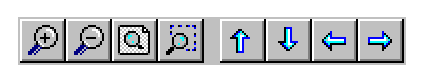
\includegraphics{belaman3.ps}}
\caption{View Manipulation toolbar buttons.}
\label{viewbuttons}
\end{figure}
The meaning of the View Manipulation toobar buttons are:
\begin{itemize}
\item The arrows on the toolbar correspond to moving the view in the direction of
the arrow approximately $1/2$ of the current screen width.
\item The ``blank page'' button scales the screen to the smallest
possible view that displays the entire problem geometry.
\item The ``+'' and ``-'' buttons zoom the current view in and
out, respectively.
\item The ``page with magnifying glass'' button allows the view to
be zoomed in on a user-specified part of the screen.  To use this
tool, first push the toolbar button.  Then, move the mouse pointer
to one of the desired corners of the ``new'' view.  Press and hold
the left mouse button.  Drag the mouse pointer to the opposite
diagonal corner of the desired ``new'' view.  Last, release the
left mouse button.  The view will zoom in to a window that best
fits the user's desired window.
\end{itemize}

Some infrequently used view commands are also available, but only
as options off of the {\tt Zoom} selection of the main menu.  This
menu contains all of the manipulations available from the toolbar
buttons, plus the options {\tt Keyboard}, {\tt Status Bar}, and
{\tt Toolbar}.

The {\tt Keyboard} selection allows the user to zoom in to a window
in which the window's corners are explicitly specified by the user
via keyboard entry of the corners' coordinates.  When this
selection is chosen, a dialog pops up prompting for the locations
of the window corners.  Enter the desired window coordinates and
hit ``OK''.  The view will then zoom to the smallest possible
window that bounds the desired window corners.  Typically, this
view manipulation is only done as a new drawing is begun, to
initially size the view window to convenient boundaries.

The {\tt Status Bar} selection can be used to hide or show the
one-line status bar at the bottom of the femm window.  Generally,
it is desirable for the toolbar to be displayed, since the current
location of the mouse pointer is displayed on the status line.

The {\tt Toolbar} selection can be used to hide or show the toolbar
buttons.  The toolbar is not fundamentally necessary to running
femm, because any selection on the toolbar is also available via
selections off of the main menu.  If more space on the screen is
desired, this option can be chosen to hide the toolbar.  Selecting
it a second time will show the toolbar again.  It may be useful to
note that the toolbar can be undocked from the main screen and made
to ``float'' at a user-defined location on screen.  This is done by
pushing the left mouse button down on an area of the toolbar that
is not actually a button, and then dragging the toolbar to its
desired location.  The toolbar can be docked again by moving it
back to its original position.

\subsection{Grid Manipulation} \label{grid_manipulation}

To aid in drawing your geometry, a useful tool is the Grid.  When
the grid is on, a grid of light blue pixels will be displayed on
the screen.  The spacing between grid points can be specified by
the user, and the mouse pointer can be made to ``snap'' to the
closest grid point.

The easiest way to manipulate the grid is through the used of the
Grid Manipulation toolbar buttons.  These buttons are pictured in
Figure~\ref{gridbuttons}.
\begin{figure}[ht]
\centerline{\includegraphics{gridbtn.ps}}
\caption{Grid Manipulation toolbar buttons.}
\label{gridbuttons}
\end{figure}
The left-most button in Figure~\ref{gridbuttons} shows and hides
the grid.  The default is that the button is pushed in, showing the
current grid.  The second button, with an icon of an arrow pointing
to a grid point, is the ``snap to grid'' button.  When this button
is pushed in, the location of the mouse pointer is rounded to the
nearest grid point location.  By default, the ``snap to grid''
button is not pressed.  The right-most button brings up the Grid
Properties dialog. This dialog is shown in Figure~\ref{griddialog}.
\begin{figure}[ht]
\centerline{\includegraphics{griddlg.ps}}
\caption{Grid Properties dialog.}
\label{griddialog}
\end{figure}

The Grid Properties dialog has an edit box for the user to enter
the desired grid sizing.  When the box appears, the number in this
edit box is the current grid size.  The edit box also contains a
drop list that allows the user to select between Cartesian and
Polar coordinates.  If Cartesian is selected, points are specified
by their (x,y) coordinates for a planar problem, or by their (r,z)
coordinates for an axisymmetric problem.  If Polar is selected,
points are specified by an angle and a radial distance from the
origin.  The default is Cartesian coordinates.

\subsection{Edit} \label{coffee}

Several useful tasks can be performed via the {\tt Edit} menu off
of the main menu.

Perhaps the most frequently used is the {\tt Undo} command.
Choosing this selection undoes the last addition or deletion that
the user has made to the model's geometry.

For selecting many objects quickly, the {\tt Select Group} command
is useful.  This command allows the user to select objects of the
current type located in an arbitrary rectangular box.  When this
command is selected, move the mouse pointer to one corner of the
region that is to be selected.  Press and hold the left mouse
button.  Then, drag the mouse pointer to the opposite diagonal
corner of the region.  A red box will appear, outlining the region
to be selected.  When the desired region has been specified,
release the left mouse button.  All objects of the current type
completely contained within the box will become selected.

Any objects that are currently selected can be moved, copied, or
pasted.  To move or copy selected objects, simply choose the
corresponding selection off of the main menu's {\tt Edit} menu. A
dialog will appear prompting for an amount of displacement or
rotation.

\subsection{Problem Definition}

The definition of problem type is specified by choosing the {\tt
Problem} selection off of the main menu.  Selecting this option
brings up the Problem Definition dialog, shown in
Figure~\ref{problemdefinition}
\begin{figure}[ht]
\centerline{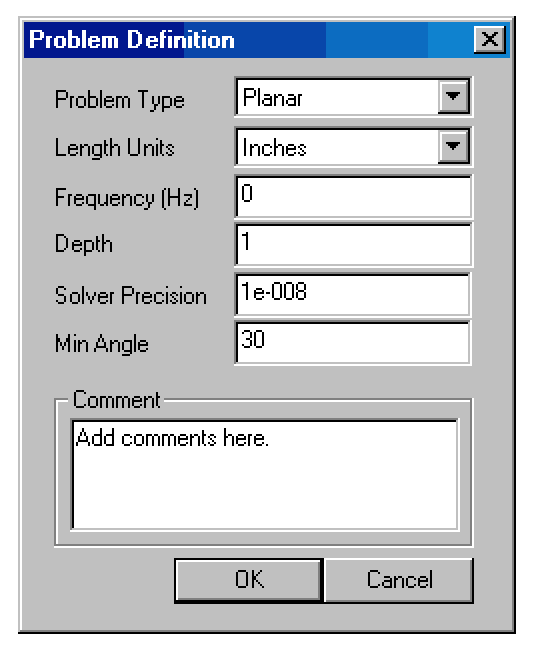
\includegraphics{probdef.ps}}
\caption{Problem Definition dialog.}
\label{problemdefinition}
\end{figure}

The first selection is the {\tt Problem Type} drop list.  This
drop box allows the user to choose from a 2-D planar problem (the
{\tt Planar} selection), or an axisymmetric problem (the {\tt
Axisymmetric} selection).

Next is the {\tt Length Units} drop list.  This box identifies what
unit is associated with the dimensions prescribed in the model's
geometry.  Currently, the program supports inches, millimeters,
centimeters, meters, mils, and $\mu$meters.

The first edit box in the dialog is {\tt Frequency (Hz)}.  For a
magnetostatic problem, the user should choose a frequency of zero.
If the frequency is non-zero, the program will perform a harmonic
analysis, in which all field quantities are oscillating at this
prescribed frequency.  The default frequency is zero.

The second edit box is the {\tt Depth} specification.  If a Planar
problem is selected, this edit box becomes enabled.  This value is
the length of the geometry in the ``into the page'' direction.
This value is used for scaling integral results in the post
processor ({\em e.g.} force, inductance, etc.) to the appropriate
length.  The units of the Depth selection are the same as the
selected length units.  For files imported from version 3.2, the
Depth is chosen so that the depth equals 1 meter, since in version
3.2, all results from planar problems ar e reported per meter.

The third edit box is the {\tt Solver Precision} edit box. The number in this edit box
specifies the stopping criteria for the linear solver.  The linear algebra
problem could be represented by:
\begin{displaymath}
M x=b
\end{displaymath} where $M$ is a square matrix, $b$ is a vector, and $x$ is
a vector of unknowns to be determined.  The solver precision value
determines the maximum allowable value for $||b-M x||/||b||$.  The
default value is $10^{-8}$.

The fourth edit box is labeled {\tt Min Angle}.  The entry in this box is used as a
constraint in the Triangle meshing program.  Triangle adds points to the mesh to
ensure that no angles smaller than the specified angle occur. If the minimum angle
is 20.7 degrees or smaller, the triangulation algorithm is theoretically guaranteed to
terminate (assuming infinite precision arithmetic -- Triangle may
fail to terminate if you run out of precision).  In practice, the
algorithm often succeeds for minimum angles up to 33.8 degrees.
For highly refined meshes, however, it may be necessary to reduce
the minimum angle to well below 20 to avoid problems associated
with insufficient floating-point precision.  The edit box will accept
values between 1 and 33.8 degrees.


Lastly, there is an optional {\tt Comment} edit box.  The
user can enter in a few lines of text that give a brief description
of the problem that is being solved.  This is useful if the user is
running several small variations on a given geometry.  The comment
can then be used to identify the relevant features for a particular
geometry.





\subsection{Definition of Properties}

To make a solvable problem definition, the user must identify
boundary conditions, block materials properties, and so on.  The
different types of properties defined for a given problem are
defined via the {\tt Properties} selection off of the main menu.

When the {\tt Properties} selection is chosen, a drop menu appears
that has selections for Materials, Boundary, Point, and Circuits.
When any one of these selections is chosen, the dialog pictured in
Figure~\ref{propertydef} appears.
\begin{figure}[ht]
\centerline{\includegraphics{propdef.ps}}
\caption{Property Definition dialog box}
\label{propertydef}
\end{figure}
This dialog is the manager for a particular type of properties. All
currently defined properties are displayed in the {\tt Property
Name} drop list at the top of the dialog.  At the beginning of a
new model definition, the box will be blank, since no properties
have yet been defined.  Pushing the {\tt Add Property} button
allows the user to define a new property type. The {\tt Delete
Property} button removes the definition of the property currently
in view in the {\tt Property Name} box.  The {\tt Modify Property}
button allows the user to view and edit the property currently
selected in the {\tt Property Name} box. Specifics for defining
the various property types are addressed in the following
subsections.

In general, a number of these edit boxes prompt the user for both
real and imaginary components for entered values.  If the problem
you are defining is magnetostatic (zero frequency), enter the
desired value in the box for the real component, and leave a zero
in the box for the imaginary component. The reason that femm uses
this formalism is to obtain a relatively smooth transition from
static to time-harmonic problems.  Consider the definition of the
{\em Phasor transformation} in Eq.~\ref{phasor_transformation}. The
phasor transformation assumes that all field values oscillate in
time at a frequence of $\omega$. The phasor transformation takes
the cosine part of the field value and represents it as the real
part of a complex number.  The imaginary part represents the
magnitude of the sine component, $90^o$ out of phase.  Note what
happens as the frequency goes to zero:
\be \lim_{\omega \rightarrow 0} \left( a_{re} \cos \omega t - a_{im} \sin
\omega t \right) = a_{re} \ee
Therefore, the magnetostatic ($\omega=0$) values are just described
by the real part the specified complex number.

\subsubsection{Point Properties}

If a new point property is added or an existing point property
modified, the {\tt Nodal Property} dialog box appears.  This dialog
box is pictured in Figure~\ref{nodalprop}
\begin{figure}[ht]
\centerline{\includegraphics{nodeprop.ps}}
\caption{Nodal Property dialog.}
\label{nodalprop}
\end{figure}

The first selection is the {\tt Name} edit box.  The default name
is ``New Point Property,'' but this name should be changed to
something that describes the property that you are defining.

Next are edit boxes for defining the vector potential, $A$, at a
given point, or prescribing a point current, $J$, at a given point.
The two definitions are mutually exclusive.  Therefore, if there
is a nonzero value the $J$ box, the program assumes
that a point current is being defined.  Otherwise, it is assumed
that a point vector potential is being defined.

There is an edit box for vector point vector potential, $A$.  A
can be defined as a complex value, if desired. The units of
$A$ are Weber/Meter.  Typically, $A$ needs to be
defined as some particular values (usually zero) at some point in
the solution domain for problems with derivative boundary
conditions on all sides.  This is the typical use of defining a
point vector potential.

Lastly, there is an edit box for the definition of a point
current, $J$.  The units for the point current are
in Amperes.  The value of $J$ can be defined as complex, if desired.

\subsubsection{Boundary Properties}

The {\tt Boundary Property} dialog box is used to specify the
properties of line segments or arc segments that are to be
boundaries of the solution domain.  When a new boundary property is
added or an existing property modified, the {\tt Boundary Property}
dialog pictured in Figure~\ref{boundaryprop} appears.
\begin{figure}[ht]
\centerline{\includegraphics{bdryprop.ps}}
\caption{Boundary Property dialog.}
\label{boundaryprop}
\end{figure}

The first selection in the dialog is the {\tt Name} of the
property.  The default name is ``New Boundary,'' but you should
change this name to something more descriptive of the boundary that
is being defined.

The next selection is the {\tt BC Type} drop list.  This specifies
the boundary condition type.  Currently, FEMM supports the
following types of boundaries:
\begin{itemize}
\item {\tt Prescribed A}
With this type of boundary condition, the vector potential, $A$, is
prescribed along a given boundary.  This boundary condition can be
used to prescribe the flux passing normal to a boundary, since the
normal flux is equal to the tangential derivative of $A$ along the
boundary.  The form for $A$ along the boundary is specified via the
parameters $A_0$, $A_1$, $A_2$ and $\phi$ in the
{\tt Prescribed A parameters} box.  If the problem is planar, the
parameters correspond to the formula:
\be A=(A_0 + A_1 x + A_2 y) e^{j \phi} \ee
If the problem type is axisymmetric, the parameters correspond to:
\be A=(A_0 + A_1 r + A_2 z) e^{j \phi} \ee
\item {\tt Small Skin Depth}
This boundary condition denotes an interface with a material
subject to eddy currents at high enough frequencies such that the
skin depth in the material is very small.  A good discussion of the
derivation of this type of boundary condition is contained in
\cite{Hoole}.  The result is a Robin boundary condition with
complex coefficients of the form:
\be \frac{\partial A}{\partial n} + \left( \frac{1+j}{\delta} \right) A = 0 \ee
where the $n$ denotes the direction of the outward normal to the
boundary and $\delta$ denotes the skin depth of the material at the
frequency of interest.  The skin depth, $\delta$ is defined as:
\be \delta = \sqrt{\frac{2}{\omega \mu_r \mu_o \sigma}} \ee
where $\mu_r$ and $\sigma$ are the relative permeability and
conductivity of the thin skin depth eddy current material.  These
parameters are defined by specifying $\mu$ and $\sigma$ in
the {\tt Small skin depth parameters} box in the dialog.  At zero
frequency, this boundary condition degenerates to $\partial
A/\partial n=0$ (because skin depth goes to infinity).
\item {\tt Mixed}
This denotes a boundary condition of the form:
\be \left( \frac{1}{\mu_r \mu_o} \right) \frac{\partial A}{\partial n}
 + c_o A + c_1 = 0 \ee
The parameters for this class of boundary condition are specified
in the {\tt Mixed} {\tt BC} {\tt parameters} box in the dialog. By the choice
of coefficients, this boundary condition can either be a Robin or a
Neumann boundary condition. There are two main uses of this
boundary condition:
\begin{enumerate}
\item By carefully selecting the $c_0$ coefficient and specifying
$c_1 = 0$, this boundary condition can be applied to the outer
boundary of your geometry to approximate an upbounded solution
region.  For more information on open boundary problems, refer to
Appendix~\ref{open_boundary}.
\item The Mixed boundary condition can used to
set the field intensity, $H$, that flows parallel to a boundary.
This is done by setting $c_0$ to zero, and $c_1$ to the desired
value of $H$ in units of Amp/Meter. Note that this boundary
condition can also be used to prescribe $\partial A/\partial n=0$
at the boundary. However, this is unnecessary--the $1^{st}$ order
triangle finite elements give a $\partial A/\partial n=0$ boundary
condition by default.
\end{enumerate}
\item {\tt Strategic Dual Image}
This is sort of an ``experimental'' boundary condition that I have
found useful for my own purposes from time to time.  This boundary
condition mimics an ``open'' boundary by solving the problem
twice: once with a homogeneous Dirichlet boundary condition on the
SDI boundary, and once with a homogeneous Neumann condition on the
SDI boundary.  The results from each run are then averaged to get
the open boundary result.  This boundary condition should only be
applied to the outer boundary of a circular domain in 2-D planar
problems.  Through a method-of-images argument, it can be shown
that this approach yields the correct open-boundary result for
problems with no iron ({\em i.e} just currents or linear magnets
with unit permeability in the solution region).
\item{\tt Periodic}
This type of boundary condition is applied to either two segments
or two arcs to force the magnetic vector potential to be identical
along each boundary.  This sort of boundary is useful in exploiting
the symmetry inherent in some problems to reduce the size of the
domain which must be modeled.    The domain merely needs to be
periodic, as opposed to obeying more restrictive $A=0$ or $\partial
A / \partial n = 0$ line of symmetry conditions. Another useful
application of periodic boundary conditions is for the modeling of
``open boundary'' problems, as discussed in
Appendix~\ref{KelvinBC}. Often, a periodic boundary is made up of
several different line or arc segments.  A different periodic
condition must be defined for each section of the boundary, since
each periodic BC can only be applied to a line or arc and a
corresponding line or arc on the remote periodic boundary.
\item{\tt Antiperiodic}
The antiperiodic boundary condition is applied in a similar way as
the periodic boundary condition, but its effect is to force two
boundaries to be the negative of one another.  This type of
boundary is also typically used to reduce the domain which must be
modeled, {\em e.g.} so that an electric machine might be modeled
for the purposes of a finite element analysis with just one pole.
\end{itemize}

\subsubsection{Materials Properties}
The {\tt Block Property} dialog box is used to specify the
properties to be associated with block labels.  The properties
specified in this dialog have to do with the material that the
block is composed of, as well as some attributes about how the
material is put together (laminated). When a new material property
is added or an existing property modified, the {\tt Block Property}
dialog pictured in Figure~\ref{blockpropdlg} appears.
\begin{figure}
\centerline{\includegraphics{blockprop.ps}}
\caption{Block Property dialog.}
\label{blockpropdlg}
\end{figure}

As with Point and Boundary properties, the first step is to choose
a descriptive name for the material that is being described.  Enter
it in the {\tt Name} edit box in lieu of ``New Material.''

Next decide whether the material will have a linear or nonlinear B-H curve
by selecting the appropriate entry in the {\tt B-H Curve} drop list.

If {\tt Linear B-H Relationship} was selected from the drop list,
the next group of {\tt Linear Material Properties} parameters will
become enabled. FEMM allows you to specify different relative
permeabilities in the vertical and horizontal directions ($\mu_x$
for the x- or horizontal direction, and $\mu_y$ for the y- or
vertical direction).

There are also boxes for $\phi_{hx}$ and $\phi_{hy}$, which denote
the hysteresis lag angle corresponding to each direction, to be
used in cases in which linear material properties have been
specified. A simple, but surprisingly effective, model for
hysteresis in harmonic problems is to assume that hysteresis
creates a constant phase lag between B and H that is independent of
frequency. This is exactly the same as assuming that hysteresis
loop has an elliptical shape. Since the hysteresis loop is not
exactly elliptical, the perceived hysteresis angle will vary
somewhat for different amplitudes of excitation. The hysteresis
angle is typically not a parameter that appears on manufacturer's
data sheets; you have to identify it yourself from a frequency
sweep on a toroidal coil with a core composed of the material of
interest. For most laminated steels, the hysteresis angle lies
between $0^o$ and $20^o$ \cite{stoll}. This same reference also has
a very good discussion of the derivation and application of the
fixed phase lag model of hysteresis.


If {\tt Nonlinear} {\tt B-H} {\tt Curve} was selected from the drop list,
the {\tt Nonlinear} {\tt Material} {\tt Properties} parameter group becomes enabled.  To
enter in points on your B-H curve, hit the {\tt Edit B-H Curve} button.  When
the button is pushed a dialog appears that allows you to enter in
B-H data (see Figure~\ref{bhdatadlg}.
\begin{figure}[ht]
\centerline{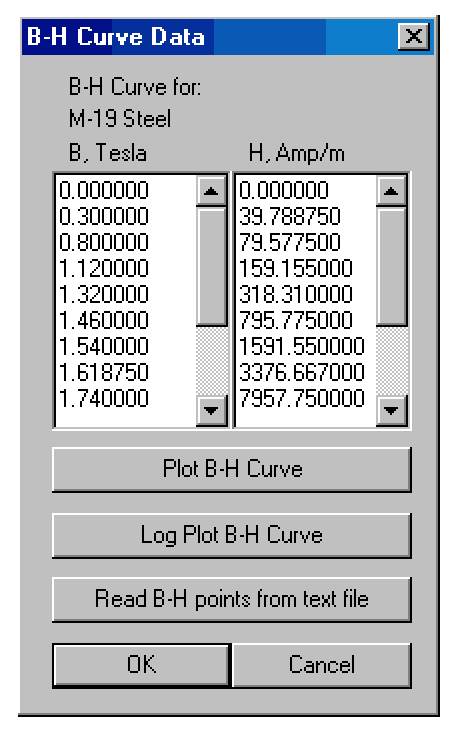
\includegraphics{bhdata.ps}}
\caption{B-H data entry dialog.}
\label{bhdatadlg}
\end{figure}
The information to be entered in these dialogs is usually obtained
by picking points off of manufacturer's data sheets.  For obvious
reasons, you must enter the same number of points in the ``B''
(flux density) column as in the ``H'' (field intensity) column.  To
define a nonlinear material, you must enter {\em at least} three
points, and you should enter ten or fifteen to get a good fit.

After you are done entering in your B-H data points, it is a good
idea to view the B-H curve to see that it looks like it is
``supposed'' to.  This is done by pressing the {\tt Plot B-H Curve}
button or the {\tt Log Plot B-H Curve} button on the B-H data dialog.
You should see a B-H curve that
looks something like the curve pictured in Figure~\ref{bhcurveplt}.
\begin{figure}[ht]
\centerline{\includegraphics{bhcurve.ps}}
\caption{Sample B-H curve plot.}
\label{bhcurveplt}
\end{figure} The boxes in the plot represent the locations of the entered
B-H points, and the line represents a cubic spline derived from the entered
data.  Since FEMM interpolates between your B-H points using cubic splines,
it is possible to get a bad curve if you haven't entered an adequate number
of points. ``Weird'' B-H curves can result if you have entered too few
points around relatively sudden changes in the B-H curve.  Femm ``takes care
of'' bad B-H data ({\em i.e.} B-H data that would result in a cubic spline
fit that is not single-valued) by repeatedly smoothing the B-H data using a
three-point moving average filter until a fit is obtained that is
single-valued.  This approach is robust in the sense that it always yields a
single-valued curve, but the result might be a poor match to the original
B-H data.  Adding more data points in the sections of the curve where the
curvature is high helps to eliminate the need for smoothing.

It may also be important to note that FEMM extrapolates linearly
off the end of your B-H curve if the program encounters flux
density/field intensity levels that are out of the range of the
values that you have entered. This extrapolation may make the
material look more permeable than it ``really'' is at high flux
densities. You have to be careful to enter enough B-H values to get
an accurate solution in highly saturated structures so that the
program is interpolating between your entered data points, rather
than extrapolating.

Also in the nonlinear parameters box is a parameter, $\phi_{hmax}$.  For
nonlinear problems, the hysteresis lag is assumed to be proportional to the
effective permeability.  At the highest effective permeability, the
hysteresis angle is assumed to reach its maximal value of $\phi_{hmax}$.
This idea can be represented by the formula:
\be \phi_h(B)= \left( \frac{\mu_{eff}(B) }{\mu_{eff,max}} \right) \phi_{hmax} \ee


The next entry in the dialog is $H_c$.  If the material is a permanent
magnet, you should enter the magnet's coercivity here in units of Amperes
per meter.  There are some subtleties involved in defining
permanent magnet properties (especially nonlinear permanent magnets).
Please refer to the Appendix~\ref{app_pm} for a more thorough discussion of
the modeling of permanent magnets in FEMM.

The next entry represents $J$, the source current density in the block. The "source current density"
denotes the current in the block at DC.  At frequencies other than DC in a region with non-zero conductivity,
eddy currents will be induced which will change the total current density so that it is no longer equal to the
source current density.  Use "circuit properties" to impose a value for the total current carried in a region
with eddy currents. Source current density can be complex valued, if desired.

The $\sigma$ edit box denotes the electrical conductivity of the
material in the block. This value is generally only used in
time-harmonic (eddy current) problems. The units for conductivity
are $10^6$ Seymens/Meter (equivalent to $10^6
(\Omega*\mbox{Meters})^{-1}$). For reference, copper at room
temperature has a conductivity of 58 MS/m; a good silicon steel for
motor laminations might have a conductivity of as low as 2 MS/m.
Commodity-grade transformer laminations are more like 9 MS/m. You
should note that conductivity generally has a strong dependence
upon temperature, so you should choose your values of conductivity
keeping this caveat in mind.

The last set of properties is the {\tt Lamination and Wire Type} section.
If the material is laminated, the drop list in this section is used to
denote the  direction in which the material is laminated.
If the material is meant to represent a bulk wound coil, this drop
list specifies the sort of wire from which the coil is constructed.

The various selections in this list are illustrated
in Figure~\ref{lamdir}
\begin{figure}[ht]
\centerline{\includegraphics{lamscheme.ps}}
\caption{Different lamination orientation options.}
\label{lamdir}
\end{figure}
Currently, the laminations are constrained to run along a
particular axis.

If some sort of laminated construction is selected in the drop list,
the lamination thickness and fill factor edit boxes become enabled.
The lamination thickness, fill factor, and lamination orientation
parameters are used to implement a bulk model of laminated
material.  The result of this model is that one can account for
laminations with hysteresis and eddy currents in harmonic problems.
For magnetostatic problems, one can approximate the effects of
nonlinear laminations without the necessity of modeling the
individual laminations separately. This bulk lamination model is
discussed in more detail in the Appendix (Section~\ref{app_lam}).

The $d_{lam}$ edit box represents the thickness of the
laminations used for this type of material.  If the material is not
laminated, enter 0 in this edit box.  Otherwise, enter the
thickness of {\em just the iron part} (not the iron plus the
insulation) in this edit box in units of millimeters.

Associated with the lamination thickness edit box is the {\tt Lam
fill factor} edit box.  This is the fraction of the core that is
filled with iron.  For example, if you had a lamination in which
the iron was 12.8 mils thick, and the insulation bewteen
laminations was 1.2 mils thick, the fill factor would be:
\begin{displaymath}
\mbox{Fill Factor} = \frac{12.8}{1.2+12.8} = 0.914
\end{displaymath}

If a wire type is selected, the {\tt Strand dia.} and/or {Number of strands}
edit boxes become enabled.  If the {\tt Magnet wire} or {\tt Square wire} types
are selected, it is understood that there is can only be one strand, and the
{\tt Number of strands} edit box is disabled.  The wire's diameter (or width)
is then entered in the {\tt Strand dia.} edit box.  For stranded and Litz wire,
one enters the number of strands and the strand diameter.  Currently, only builds
with a single strand gauge are supported.

If a wire type is specified, the material property can be applied to a ``bulk''
coil region each individual turn need not be modeled.  In DC problems, the results
will automatically be adjusted for the implied fill factor.  For AC problems, the
the fill factor is taken into account, and AC proximity and skin effect losses are
taken into account via effective complex permeability and conductivity that are
automatically computed for the wound region.

\subsubsection{Materials Library}

Since one kind of material might be needed in several different
models, FEMM has a built-in library of Block Property definitions.
The user can access and maintain this library through the {\tt
Properties | Materials Library} selection off of the main menu.
When this option is selected, the {\tt Materials Library} dialog
pictured in Figure~\ref{matlibdlg} appears.
\begin{figure}[ht]
\centerline{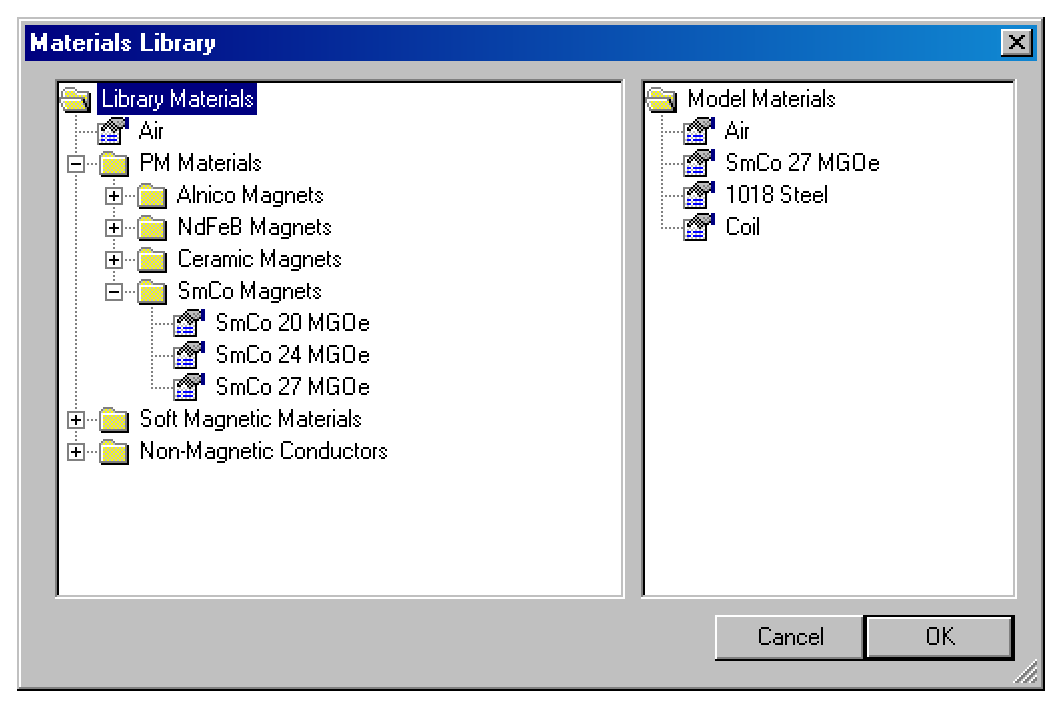
\includegraphics{fe_matlib.ps}}
\caption{Materials Library dialog.}
\label{matlibdlg}
\end{figure}
This dialog allow the user to exchange Block
Property definitions between the current model and the materials
library via a drag-and-drop interface.

A number of different options are available via a mouse button right-click
when the cursor is located on top of a material or folder. Materials can be edited
by double-clicking on the desired material.

Material from other material libraries or models can be imported by selecting the
``Import Materials'' option from the right-button menu that appears when the pointer
is over the root-level folder of either the Library or Model materials lists.

The materials library should be located in the same directory as
the FEMM executable files, under the filename \verb+mlibrary.dat+.
If you move the materials library, femm will not be able to find
it.

\subsubsection{Circuit Properties}

The purpose of the circuit properties is to allow the user
to apply constraints on the current flowing in one
or more blocks. Circuits can be defined as either ''parallel'' or
''series'' connected.

If ''parallel'' is selected, the current is
split between all regions marked with that circuit property on the
basis of impedance ({\em} current is split such that the voltage drop
is the same across all sections connected in parallel).  Only solid
conductors can be connected in parallel.

If ''series'' is selected, the specified current is applied to each block
labeled with that circuit property.  In addition, blocks that are
labeled with a series circuit property can also be assigned a number of
turns, such that the region is treated as a stranded conductor in which
the total current is the series circuit current times the number of turns
in the region.  The number of turns for a region is prescribed as a block
label property for the region of interest.  All stranded coils must be
defined as series-connected (because each turn is connected together with
the other turns in series).  Note that the number of turns assigned to
a block label can be either a positive or a negative number.  The sign
on the number of turns indicated the direction of current flow associated
with a positive-valued circuit current.

For magnetostatic problems, one could alternatively apply a source
current density over the conductor of interest and achieve similar
results. For eddy current problems, however, the ``circuit''
properties are much more useful--they allow the user to define the
current directly, and they allow the user to assign a particular connectivity
to various regions of the geometry.  This information is used to
obtain impedance, flux linkage, etc., in a relatively painless way
in the postprocessor.

By applying circuit properties, one can also enforce connectivity
in eddy current problems. By default, all objects in eddy current
problems are ``shorted together at infinity''--that is, there is
nothing to stop induced currents from returning in other sections
of the domain that might not be intended to be physically
connected.  By applying a parallel-connected circuit with a zero net current density
constraint to each physical ``part'' in the geometry, the
connectivity of each part is enforced and all is forced to be
conserved inside the part of interest.

The dialog for entering circuit properties is pictured in
Figure~\ref{circprop}.
\begin{figure}[ht]
\centerline{\includegraphics{circprop.ps}}
\caption{Circuit Property dialog}
\label{circprop}
\end{figure}

%\subsubsection{Circuit Properties}

\subsection{Exterior Region}

One often desires to solve problems on an unbounded domain.  Appendix~\ref{KelvinBC}
describes an easy-to-implement conformal mapping method for representing an unbounded
domain in a 2D planar finite element analysis.  Essentially, one models two disks--one
represents the solution region of interest and contains all of the items of interest,
around which one desires to determine the magnetic field.  The second disk represents
the region exterior to the first disk.  If periodic boundary conditions are employed to
link the edges of the two disks, it can be shown (see Appendix~\ref{KelvinBC}) that the
result is exactly equivalent to solving for the fields in an unbounded domain.

One would also like to apply the same approach to model unbounded axisymmetric problems,
as well as unbounded planar problems. Unfortunately, the Kelvin Transformation is a bit
more complicated for axisymmetric problems.  In this case, the permeability of the
external region has to vary based on distance from the center of the external region and
the outer radius of the external region.  The approach is described in detail in
\cite{LowFreeAxi}.  FEMM automatically implements the variation of permeability in the
exterior region, but a bit more information must be collected to perform the permeability
grading required in the external region.  This is where the ``External Region'' parameters
come in--these are the parameters that the program needs to define the permeabilities of
elements in the external region for ``unbounded'' axisymmetric problems.

Specifically, there are three parametes that are collected in the dialog that appears when
the user selects the External Region properties.  These are:

\begin{itemize}
\item {\tt Center of Exterior Region}  The location along the z-axis of the axisymmetric problem
where the center of the block representing the external region is located.
\item {\tt Radius of Exterior Region}  Radius of the sphere representing the exterior region.
\item {\tt Radius of Interior Region} Radious of the spehre representing the interior region
({\em i.e.} the region in which the items of interest are located).
\end{itemize}

To finish defining the axisymmetric external region, the {\tt Block located in an external region}
check box must be selected in any block labels that are located in the region that is desired to
be the axisymmetric external region.

\subsection{Analysis Tasks}

Meshing the model, analyzing the model, and viewing the results are
most easily performed by the toolbar buttons pictured in
Figure~\ref{runnybutts}
\begin{figure}[ht]
\centerline{\includegraphics{spawnbtn.ps}}
\caption{Toolbar buttons for starting analysis tasks.}
\label{runnybutts}
\end{figure}

The first of these buttons (with the ``yellow mesh'' icon) runs the
mesh generator. The solver actually automatically calls the mesh
generator to make sure that the mesh is up to date, so you never
{\em have} to call the mesher from within femm.  However, it is
almost always important to get a look at the mesh and see that it
``looks right.''  When the mesh generation button is pressed, the
mesher is called.  While the mesher is running, an entry labeled
``triangle'' will appear on the Windows taskbar.
After the geometry is triangulated, the finite element mesh is
loaded into memory and displayed underneath the defined nodes,
segments, and block labels as a set of yellow lines.

If you have a very large model, just keeping all of the mesh
information in core can take up a significant amount of memory.  If
you are about to analyze a very large problem, it might be a good
idea to choose the \verb+Mesh | Purge Mesh+ option off of the main
menu.  When this option is selected, the mesh is removed from
memory, and the memory that it occupied is freed for other uses.

The second button, with the ``hand-crank'' icon, executes the
solver, {\tt fkern.exe}. Before fkern is actually run, the Triangle
is called to make sure the mesh is up to date. Then, fkern is
called. When fkern runs, it opens up a console window to display
status information to the user. However, fkern requires no user
interaction while it is running. When fkern is finished analyzing
your problem, the console window will disappear. The time that
fkern requires is highly dependent on the problem being solved.
Solution times can range from less than a second to several hours,
depending upon the size and complexity of the problem. Generally,
linear magnetostatic problems take the least amount of time.
Harmonic problems take slightly more time, because the answer is in
terms of complex numbers. The complex numbers effectively double
the number of unknowns as compared to a magnetostatic problem with
the same mesh. The slowest problems to analyze are nonlinear
time-harmonic problems, since multiple successive approximation
iterations must be used to converge on the final solution. However,
nonlinear problems almost never take more than 10 iterations. Later
iterations in nonlinear problems are usually are quite fast
compared to the first iteration or two because the later iterations
can be initialized with an approximate solution that is very close
to the ``actual'' solution.

For users who have a technical interest in what is ``under the
hood'' in fkern, some details are provided in the Appendix
(Section~\ref{fkern_stuff}).

The ``big magnifying glass'' icon is used to display the results in
a postprocessing window once the analysis is finished.  A detailed
description of the magnetics postprocessor addressed in
Section~\ref{ppsec}.

%--------------------------------------------------------------------------------------------------
\section{Magnetics Postprocessor} \label{ppsec}

The the magnetics postprocessing functionality of femm is used to
view solutions generated by the {\tt fkern} solver.  A magnetics
postprocessor window can be opened either by loading some
previously run analyses via {\tt File|Open} on the main menu, or by
pressing the ``big magnifying glass'' icon from within a
preprocessor window to view a newly generated solution. Magnetics
postprocessor data files stored on disk have the {\tt .ans} prefix.

\subsection{Postprocessor modes} \label{tape}

Similar to the preprocessor, the postprocessor always operates in
one of three modes, depending upon the task to be performed.  These
modes are:
\begin{itemize}
\item {\em Point Values Mode} In this mode, the user can click on
various points in the solution region.  Local field values are then
listed in the {\tt FEMM Output} window.
\item {\em Contour Mode} This mode allows the user to define
arbitrary contours in the solution region.  Once a contour is
defined, plots of field quantities can be produced along the
contour, and various line integrals can be evaluated along the
contour.
\item {\em Block Mode} The Block Mode lets the user define a
subdomain in the solution region.  Once the block has been defined,
a variety of area and volume integrals can be taken over the
defined subdomain.  Integrals include stored energy (inductance),
various kinds of losses, total current in the block, and so on.
\end{itemize}

The current postprocessor mode is controlled via the Analysis Mode
toolbar buttons, shown in Figure~\ref{anal_mode}.
\begin{figure}[ht]
\centerline{\includegraphics{analmode.ps}}
\caption{Analysis Mode toolbar buttons}
\label{anal_mode}
\end{figure}
The buttons denote, respectively, Point Values mode, Contour Mode,
and Block Mode.  The depressed button denotes the current mode. The
default mode when postprocessor starts is Point Values mode.


\subsection {View and Grid Manipulation}

The aspects of the current view and of the current grid are
regulated via the use of toolbar buttons.  The view is manipulated
by the following toolbar buttons:
\begin{figure}[ht]
\centerline{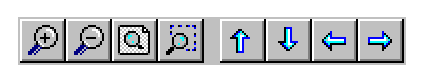
\includegraphics{belaman3.ps}}
\caption{View Manipulation toolbar buttons.}
\end{figure}
and the grid settings are manipulated by these grid manipulation
toolbar buttons:
\begin{figure}[ht]
\centerline{\includegraphics{gridbtn.ps}}
\caption{Grid Manipulation toolbar buttons.}
\end{figure}
The grid and view manipulation work in exactly the same fashion as
these same features in the preprocessor.  Refer to
Section~\ref{grid_manipulation} for a detailed description of grid
manipulation, and to Section~\ref{view_manipulation} for view
manipulation.

\subsection{Keyboard Commands}

Unlike the preprocessor, postprocessor is not very dependent on
keyboard commands.

In the Point Values mode, there is only one relevant keypress. In
this mode, the Tab key allows the user to enter the coordinates of
a specific point.  After the coordinates of a point are entered,
the field values at that point are displayed in the {\tt FEMM
Output} window.

In the Contours, there are four relevant keys. Pressing the Escape
key wipes out any current contour or block definition. Pressing the
Delete removes the last point added to the current contour or block
edge.  Pressing the Shift key allows the user to turn the last segment
in the prescribed contour from a straight line into an arc.  A dialog
pops up after the key is pressed that prompts for attributes of the
the desired arc. Last, pressing the Tab keys allows the user to numerically
enter the coordinates of a point to be included in the current
contour.

In the Block mode, the Escape and Delete keys have the same
definition as in Contours mode.  In the Block mode, the Tab key
does not do anything, since all points on the contour must also be
Points defining the model's geometry.

\subsection{Mouse Actions}

In contrast, the operation of the postprocessor is very dependent
upon input from the mouse.

In the Point Values mode, a Left Button Click is used to display
field values at the current mouse location.  If Snap to Grid is
enabled, values are displayed at the closes grid point instead.

In the Contours mode, mouse clicks are used to define the contour.
A Left Button Click adds the closest Point in the model's geometry.
Via a Right Button Click, the current mouse pointer location is
added to the contour.  A contour appears as a red line on the
screen.

Blocks are defined in Block mode in a fashion very similar to the
way in which contours are defined.  A block is defined by by
drawing a contour around the region of interest.  The contour
appears as a green line on the postprocessor screen.  When the ends
of the contour meet, the block is defined.  All elements enclosed
by the contour (all elements that form the block) then turn green
in the postprocessor window.

A Left Button Click attempts to add the nearest Point in the input
geometry to the Block's contour.  However, a block can only be
defined along line and arc segments from the input geometry.  Each
node on the boundary of the block must be selected in order to form
the Block boundary.  In Block mode, the Right mouse button has no
function.

\subsection{Miscellaneous Useful View Commands} \label{scissors}

There are some additional entries on the postprocessor {\tt View}
menu that might be useful to you from time to time.  These are:
\begin{itemize}
\item {\tt Smoothing} By default, a smoothing algorithm is applied
to the flux density solution.  Because first-order triangles are
used as trial functions for vector potential, the resulting flux
density and field intensity distributions are piece-wise constant
in each element.  The smoothing algorithm uses a nearest neighbor
interpolation to obtain linear $B$ and $H$ distributions over each
element.  The smoothed solution generally looks better on the
screen, and somewhat increases the accuracy of $B$ and $H$ near the
vertices of each element.  However, if you want to toggle
smoothing, this can be done by selecting the {\tt Smoothing}
option.
\item {\tt Show Points}  Especially when making graphics for
reports, presentations, etc, it may be desirable to hide the small
boxes on the screen that denote input node points.  The {\tt Show
Points} option allows the user to toggle whether or not the input
points are shown.
\item {\tt ToolBar} Use this toggle to hide and show the floating
toolbar.
\item {\tt Point Props} Use this toggle to hide and show the
floating dialog box used to display point property information.
\end{itemize}


\subsection{Contour Plot}

One of the most useful ways to get a subjective feel for a
magnetics finite element solution is by plotting the ``flux
lines.''  These are the streamlines along which flux flows in the
finite element geometry.  Where flux lines are close together, the
flux density is high.  In FEMM's vector potential formulation, flux
lines are simply plots of the level contours of the vector
potential, $A$, in planar problems, or level contours of $2
\pi r A$ in axisymmetric problems.

For harmonic problems, the contours are a little more subtle--$A$
has both real and imaginary components.  In this case,
postprocessor allows the user to plot contours of either the real
or the imaginary part of $A$.  Real contours appear black, and
Imaginary contours appear as grey.

By default, a set of 19 flux lines are plotted when a solution is
initially loaded into postprocessor.  The number and type of flux
lines to be plotted can be altered using the Contours Plot icon in
the Graph Mode section of the toolbar (see Figure~\ref{graph_mode}.
The Contour Plot icon is the icon with the black contours.
\begin{figure}
\centerline{\includegraphics{hplotbar.ps}}
\caption{Graph Mode toolbar buttons.}
\label{graph_mode}
\end{figure}
When this button is pressed, a dialog pops up, allowing the choice
of the number of contours (between 4 and 100 are allowed), and
which contours to plot (either real, imaginary, or none).

In the contour plot dialog, a check box is also present titled
``Show stress tensor mask''. If this box is checked, the contour
lines associated with the last Weighted Stress Tensor integration
are also displayed, by default as orange flux lines.

\subsection{Density Plot}
Density plots are also a useful way to get a quick feel for the
flux density in various parts of the model.  A density plot can be displayed
by pressing the middle button in
the Graph Mode section of the toolbar (see
Figure~\ref{graph_mode}).  A dialog the pops up that allows the
user to turn density plotting on.  The user can choose to plot
flux density, field intensity, or current density. If the solution is to a harmonic
problem, the user can choose to plot either the magnitude or just the real
or imaginary part of these quantities.

The flux density at each point is classified into one of twenty contours
distributed evenly between either the minimum and maximum flux densities or
user-specified bounds.

\subsection{Vector Plots}
A good way of getting a feel for the direction and magnitude of the
field is with plots of the field vectors. With this type of plot
arrows are plotted such that the direction of the arrow indicates
the direction of the field and the size of the arrow indicates the
magnitude of the field. The presence and appearance of this type of
plot can be controlled by pressing the ``arrows'' icon pictured in
Figure~\ref{graph_mode}.

\subsection{Line Plots}

When postprocessor is in Contours Mode, various field values of
interest can be plotted along the defined contour.  A plot of a
field value defined contour is performed by pressing the ``graphed
function'' icon in the Plot, Integration, and Circuit Results group of toolbar
buttons, shown in Figure~\ref{choadbar}.
\begin{figure}
\centerline{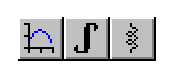
\includegraphics{intplot.ps}}
\caption{Line Plot, Integration, and Circuit Results toolbar buttons}
\label{choadbar}
\end{figure}
When this button is pressed, the {\tt X-Y Plot} dialog (see
Figure~\ref{plot_dlg}) appears with a drop list containing the
types of line plots available. Choose the desired type of plot and
press ``OK.''
\begin{figure}[ht]
\centerline{\includegraphics{pltdlg.ps}}
\caption{X-Y Plot dialog.}
\label{plot_dlg}
\end{figure}

After ``OK'' is pressed, the program computes the desired values
along the defined contour.  These values are then plotted using the
{\tt femmplot} program, which is called automatically to display
the plot.

By default, the {\tt Write data to text file} box is not checked.
If the user selects this option, the file selection dialog will
appear and prompt for a filename to which to write the data. The
data is written in two-column text format.  If {\tt Write data to
text file} is selected, a femmplot window will not appear.

Currently, the type of line plots supported are:
\begin{itemize}
\item Vector potential along the contour;
\item Magnitude of the flux density along the contour;
\item Component of flux density normal to the contour;
\item Component of flux density tangential to the contour;
\item Magnitude of the field intensity along the contour;
\item Component of field intensity normal to the contour;
\item Component of field intensity tangential to the contour;
\end{itemize}

In all of these plots, the direction of the normal is understood to
be as shown in Figure~\ref{this_side}.  The tangential direction is
understood to be the direction in which the contour was defined.
\begin{figure}[ht]
\centerline{\includegraphics{thisside.ps}}
\caption{When in doubt plots and integrals taken on this side of a contour.}
\label{this_side}
\end{figure}

In certain cases, the quantity to be plotted can be ambiguous. This
can occur, for example, if a plot of the tangential field intensity
is requested on a contour running along an interface between air
and a piece of iron.  In this case, there is a discontinuity in the
tangential field intensity, and the value of this quantity is
different on each side of the interface.  The postprocessor
resolves the conflict by always evaluating the plots at a
differentially small distance to the ``normal'' side of the line.
Therefore, by defining the same contour but reversing the order in
which the points are specified, plots of the quantity of interest
on each side of a boundary can be obtained.




\subsection{Line Integrals}

Once a contour has been specified in Contours mode, Line Integrals
can be performed along the specified contour.  These integrals are
performed by evaluating a large number of points at evenly spaced
along the contour and integrating using a simple trapezoidal-type
integration scheme.

To perform an integration, press the ``integral'' icon on the
toolbar (as shown in Figure~\ref{choadbar}).  A small dialog will
appear with a drop list.  Choose the desired integral from the drop
list and press {\tt OK}.  The amount of time required to perform
the integral will be virtually instantaneous for some types of
integrals; however, some types may require several seconds to
evaluate.  When the evaluation of the integral is completed, the
answer appears on the screen in a pop-up box.

One ``tip'' that may aid with the definition of contours of integration is
that a curved integration contour can be defined in a fairly painless
fashion by hitting the Shift key.  Hitting the Shift key tells the program
to turn the last segment in the defined integration contour into an arc
segment.  A dialog then pops up that prompts for the desired attributes of
the arc.

The line integrals currently supported are:
\begin{itemize}
\item {\tt B.n}.  This integral returns the total flux passing normal
to the contour.  This integral is useful for determining the total
flux in a bulk flux path.  This result might then be compared to
predictions from a simpler magnetic circuit model, for example.
\item {\tt H.t}. The integral of the tangential field intensity along
the contour yields the magnetomotive force drop between the
endpoints of the contour.  Again, this integral is useful for
comparison to or validation of magnetic circuit models.
\item {\tt Contour Length}.  This integral returns the length of
the defined contour in meters.
\item {\tt Force from stress tensor}.  This integral totals the
force produced on the contour derived from Maxwell's stress tensor.
Deriving meaningful force results requires some care in the choice
of integration path; refer to Section~\ref{maxforce} for a detailed
discussion of force and torque calculation.
\item {\tt Torque from stress tensor}.  This selection integrates
the torque about the point (0,0) inferred from Maxwell's stress
tensor.  Again, some guidelines must be followed to get accurate
torque results (see Section~\ref{maxforce}).
\item \verb+B.n^2+.  This selection evaluates the integral of the
square of the normal flux along the line.  This integral is not so
commonly used, but it has been useful in the past for some
specialized purposes, like determining the RMS amplitude of a
periodic flux distribution.
\end{itemize}

\subsection{Block Integrals}
Once a closed contour has been specified in Block mode and the
block appears highlighted in green, Block Integrals over the
specified area. These integrals are performed by analytically
integrating the specified kernel over each element in the defined
region, and summing the results for all elements.

To perform an integration, press the ``integral'' icon on the
toolbar (as shown in Figure~\ref{choadbar}).  A small dialog will
appear with a drop list.  Choose the desired integral from the drop
list and press {\tt OK}.  Generally, volume integrals take several
seconds to evaluate, especially on dense meshes.  Be patient. When
the evaluation of the integral is completed, the answer appears on
the screen in a pop-up box.

The block integrals currently supported are:
\begin{itemize}
\item {\tt A.J}  This integral is the evaluation of $\int A \cdot J
dV$ that is usually used evaluate inductance for linear problems.
Generally, the self-inductance of a coil is:
\be L_{self}= \frac{\int A \cdot J dV}{i^2} \ee
where $i$ is the current flowing through the coil.
\item {\tt A}  This integral, the evaluation of $\int A dV$, can be used to evaluate mutual
inductances between coils.  Similar to the formula for self
inductance, mutual inductance is:
\be \label{lmut} L_{mutual} = \frac{\int A_1 \cdot J_2 dV_2}{i_1 i_2} \ee
where $A_1$ is the component of $A$ produced by the first coil,
$J_2$ is the current in the second coil, and $i_1$ and $i_2$ are
the current in the first and second coils, respectively.  $dV_2$ is
meant to denote that the integral is taken over the volume of the
second coil.  We can rearrange~(\ref{lmut}) into a somewhat simpler
form by noting that $n_2 * i_2 = J_2 * a_2$.  That is, the total
amps times turns for the second coil equals the current density in
the second coil times the second coil's cross-section area.
Substituting for $J_2$ in~(\ref{lmut}) yields:
\be \label{lmut2}
L_{mutual} = \frac{n_2}{i_1 a_2} \left(\int_{J_{2+}} A_1 dV_2 -
\int_{J_{2-}} A_1 dV_2 \right)
\ee where the first bracketed term in~(\ref{lmut2}) is the contribution from
the turns of coil 2 that are pointed out of the page and the second
term is the contribution from the turns of coil 2 that are pointed
into the page.  To evaluate mutual inductance with FEMM, one
substitutes values into~(\ref{lmut2}). First, run the model with
only ``coil 1'' turned on. Then, integrate $A$ over the volume in
which the second coil lies (although the second coil is not turned
on). For planar problems, you will typically have to make two
separate integrations--one over the region where the turns in
``coil 2'' are pointed out of the page ({\em i.e.} that part of the
coil in which a positive current results in current flowing in the
out-of-the-page direction), and one over the region in which the
turns in ``coil 2'' are pointed into the page.  Add these two
results together to get the total $A_1 dV_2$ integral. Lastly,
multiply the integral result times $n_2/(i_1 a_2)$ to get mutual
inductance.
\item {\tt Magnetic field energy} This selection calculates the energy
stored in the magnetic field in the specified region.  This
integral can be used as an alternate method of getting inductance
for problems that are linear (at least not heavily saturated).
Denoting $E$ as the energy stored in the magnetic field, inductance
can be obtained by solving the formula:
\be E = \frac{L i^2}{2} \ee
In the case of nonlinear materials, the energy is computed via:
\be W \ = \int \left( \int_0^B H(B') dB' \right) dV \ee
to take proper account of the energy under nonlinear conditions
\item{\tt Magnetic field coenergy} For linear problems, coenergy
is numerically the same as energy.  For nonlinear problems,
coenergy is defined as:
\be W_c \ = \int \left( \int_0^H B(H') dH' \right) dV \ee
Coenergy can be used in an alternative method of force and torque
computation. To compute force via coenergy, currents are held
constant, and the position of the object upon which the force is
desired is perturbed slightly. The force can then be estimated by:
\be \label{coenergyforce} F=\frac{W_c(p+\delta) - W_c(p)}{\delta} \ee
where $p$ denotes the initial position, $p+\delta$ denotes the
perturbed position, and $\delta$ is the magnitude of the
perturbation.  The component of force determined in this way acts
along the direction of the perturbation--one has to perform two
such operations to get both horizontal and vertical components of
the force.
\item {\tt Hyst. and/or Laminated eddy current losses}.  This
selection is typically used to obtain the core losses produced in
laminated iron sections in harmonic problems.
\item {\tt Resistive losses}  This selection integrates the $i^2R$
losses due to currents flowing in the ``$z$'' direction (or
$\theta$ direction, if you are evaluating an axisymmetric problem).
\item {\tt Block cross-section area}
\item {\tt Total losses} This selection totals the losses from all
possible loss mechanisms that might apply over the given block.
This is especially useful for finding losses in a region that might
enclose several different types of materials with different loss
mechanisms.
\item {\tt Lorentz force (JxB)}  Lorentz force is the force
produced by a magnetic field acting upon a current:
\be F_{Lorentz}=\int J \times B \, dV \ee Many
devices ({\em e.g.} voice coil actuators) produce forces in a
fashion that can be evaluated using this integral.
\item {\tt Lorentz torque (rxJxB)}  This selection computes the
torque about $(0,0)$ resulting from Lorentz forces.
\item {\tt Integral of B over block}  This integral can be useful
in computing Lorentz forces.  Since Lorentz force is $J \times B$,
the force that would be produced if a coil were placed in a certain
part of the solution domain can be inferred by integrating $B$, and
then scaling times an arbitrarily chosen current density to get
force.
\item {\tt Total current}  This integral returns the total
specified currents in the given block.
\item {\tt Block Volume} For axisymmetric problems, this selection
returns the volume swept out by the selected block.
\item {\tt Force via Weighted Stress Tensor} The Weighted Stress
Tensor block is a volume integral version of Maxwell's stress
tensor that automatically picks a collection of paths for the
integration that yield ``good'' force results. This approach is
similar to the weighted stress tensor approach described in
\cite{mcfee} and/or \cite{henforce}.

To compute the force on a region or set of regions, the user
selects the blocks upon which force result is desired and selects the {\tt Force via Weighted Stress Tensor} integral.  The
program then computes the weighting function by solving an
additional Laplace equation over the air surrounding the blocks upon which the force is to be computed.
It may take a few seconds to compute the weighting
function--progress is be indicated by a progress bar that is
displayed while the weighting function is being computed. The
stress tensor is then evaluated as a volume integration, and the
results are displayed.  The results are typically more accurate
than the Maxwell Stress Tensor line integral, since in some sense,
all possible contours have been averaged to yield the Weighted
Stress Tensor force result.

If the user is interested in the contours along which the integral
was performed, the "stress tensor mask" box can be checked in the
contour plot dialog.  A set of orange (by default) lines will be
displayed that.

\item {\tt Torque via Weighted Stress Tensor}  This integral is
torque version of the {\tt Force via Weighted Stress Tensor}
integral. Instead of force, torque about (0,0) is computed using
the same weighting function approach.

\item \verb+R^2 (i.e. Moment of Inertia/density)+  This integral is
used to determine the moment of inertial of the selected blocks.  To
obtain moment of inertia, the result of this integral must be multiplied
by the density of the selected region.  For 2D planar problems, the
moment of inertia about the z-axis ({\em i.e.} about x=0,y=0) is computed.
For axisymmetric problems, the integral is computed about the r=0 axis.

\end{itemize}

\subsection{Force/Torque Calculation} \label{maxforce}

Ultimately, the estimation of magnetically produced forces and
torques is often the goal of a finite element analysis.  This
section discusses some of the different methods of deducing forces
and torques using FEMM.

\subsubsection{Lorentz Force/Torque}
If one is attempting to compute the force on a collection of
currents in a region containing {\em only} materials with a unit
relative permeability, the volume integral of Lorentz torque is
always the method to employ.  Lorentz force results tend to be
very accurate.  However, again, they are only applicable for the
forces on conductors of with unit permeability ({\em e.g.} coils
in a voice coil actuator).

\subsubsection{Weighted Stress Tensor Volume Integral}
This volume integral greatly simplifies the computation of forces
and torques, as compared to evaluating forces via the stress tensor
line integral of differentiation of coenergy. Merely select the
blocks upon which force or torque are to be computed and evaluate
the integral. No particular ``art'' is required in getting good
force or torque results (as opposed to the Stress tensor line
integral), although results tend to be more accurate with finer
meshing around the region upon which the force or torque is to be
computed.

One limitation of the Weighted Stress Tensor integral is that the
regions upon which the force is being computed must be entirely
surrounded by air and/or abutting a boundary. In cases in which the
desired region abuts a non-air region, force results may be deduced
from differentiation of coenergy--see (\ref{coenergyforce}).

\subsubsection{Maxwell Stress Tensor Line Integral}
The indiscriminate use Maxwell's Stress Tensor can result in bad
predictions forces and  torques.  The goal of this section is to
explain how to set up problems and properly choose integration
paths so that good estimations of force and torque might be
obtained via stress tensor methods.  Generally, you should not
use the Stress Tensor line integral to compute forces and torques
if it can be avoided ({\em i.e.} use the volume integral version instead).

Maxwell's stress tensor prescribes a force per unit area produced
by the magnetic field on a surface.  The differential force
produced is:
\be \label{stresstensor} dF= \mbox{$\frac{1}{2}$} \left(
H(B \cdot n) + B(H \cdot n) - (H \cdot B) n \right) \ee where $n$
denotes the direction normal to the surface at the point of
interest.  The net force on an object is obtained by creating a
surface totally enclosing the object of interest and integrating
the magnetic stress over that surface.

While an integration of (\ref{stresstensor}) theoretically gives
the magnetic force on an object, numerical problems arise when
trying to evaluate this integral on a finite element mesh made of
first-order triangles.  Though the solution for vector potential
$A$ is relatively accurate, the distributions of $B$ and $H$ are an
order less accurate, since these quantities are obtained by
differentiating the trial functions for $A$.  That is, $A$ is
described by a linear function over each element, but $B$ and $H$
are piece-wise constant over each element.  Errors in $B$ and $H$
can be particularly large in elements in which the exact solution
for $B$ and $H$ changes rapidly--these areas are just not well
approximated by a piece-wise approximation.  Specifically, large
errors can arise in the tangential components of $B$ and $H$ in
elements adjacent to boundaries between materials of different
permeabilites.  The worst errors arise on this sort of interface at
corners, where the exact solution for $B$ is nearly a singularity.

If the stress tensor integral is evaluated on the interface between
two different materials, the results will be particularly
erroneous. However, the stress tensor has the property that, for an
exact solution, the same result is obtained regardless of the path
of integration, as long as that path encircles the body of interest
and passes only through air (or at least, every point in the
contour is in a region with a constant permeability). This implies
that the stress tensor can be evaluated over a contour a few
elements away from the surface of an object--where the solution for
$B$ and $H$ is much more accurate. Much more accurate force results
will be obtained by integrating along the contour a few elements
removed from any boundary or interface. The above discussion is the
rationale for the first guideline for obtaining forces via stress
tensor:

\begin{quote}
Never integrate stress stress tensor along an interface between
materials.  Always define the integration contour as a closed path
around the object of interest with the contour displaced several
elements (at least two elements) away from any interfaces or
boundaries.
\end{quote}

As an example of a properly defined contour, consider
Figure~\ref{mcont1}.
\begin{figure}
\centerline{\includegraphics{mcontour1.ps}}
\caption{Properly defined contour for integration of Maxwell's
Stress Tensor}
\label{mcont1}
\end{figure}
This figure represents a horseshoe magnet acting on a block of
iron.  The objective is to obtain the magnetic forces acting upon
the iron block.  The red line in the figure represents the contour
defined for the integration.  The contour was defined running
clockwise around the block, so that the normal to the contour
points outward.  Always define your contour in a clockwise
direction to get the correct sign.  Note that the contour is well
removed from the surface of the block, and the contour only passes
through air.  To aid in the definition of a closed contour, grid
and the ``snap to grid'' were turned on, and the corners of the
contour are grid points that were specified by right mouse button
clicks.

The second rule of getting good force results is:
\begin{quote}
Always use as fine a mesh as possible in problems where force
results are desired.
\end{quote}
Even though an integration path has been chosen properly (away from
boundaries and interfaces), some significant error can still arise
if a coarse mesh is used.  Note that (\ref{stresstensor}) is
composed of $B^2$ terms -- this means that stress tensor is one
order worse in accuracy than $B$.  The only way to get that
accuracy back is to use a fine mesh density.  A good way to proceed
in finding a mesh that is ``dense enough'' is to solve the problem
on progressively finer meshes, evaluating the force on each mesh.
By comparing the results from different mesh densities, you can get
and idea of the level of accuracy (by looking at what digits in the
answer that change between various mesh densities). You then pick
the smallest mesh density that gives convergence to the desired
digit of accuracy.

For torque computations, all the same rules apply as for force
computations ({\em i.e.} define integration contours away from
boundaries and interfaces, and use a dense mesh).

\subsection{Circuit Results}

If ``circuit'' properties are used to specify the excitation, a
number of useful properties relative to the circuit are automatically
available.
To view the circuit results, either press the "Circuit Results"
button on the toolbar pictured in Figure~\ref{choadbar}
or select \verb+View|Circuit+ Props off
of the postprocessor main menu. A dialog, as pictured in
Figure~\ref{circuitresults} will appear. There is a drop list on
the dialog, from which the user selects the circuit for which
results are desired.
\begin{figure}
\centerline{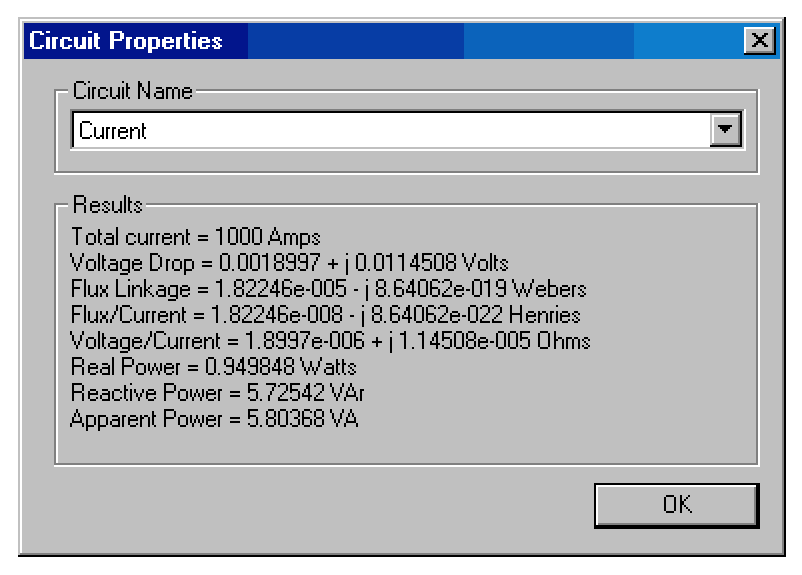
\includegraphics{circuitrslt.ps}}
\caption{Circuit results dialog.}
\label{circuitresults}
\end{figure}



%------------------------------------------------------------------------------------
\section{Electrostatics Preprocessor}

The preprocessor is used for drawing the problems geometry, defining
materials, and defining boundary conditions. The process of construction of electrostatics
problems is mechanically nearly identical to the construction of
magnetics problems--refer to Sections~\ref{pencil} through~\ref{coffee} for
an overview of the FEMM editing and problem creation commands. This section
considers those parts of problem definition that are unique to electrostatics problems.

\subsection{Problem Definition}

The definition of problem type is specified by choosing the
\texttt{Problem} selection off of the main menu. Selecting this
option brings up the Problem Definition dialog, shown in
Figure~\ref{fig6}.

\begin{figure}[htbp]
\centerline{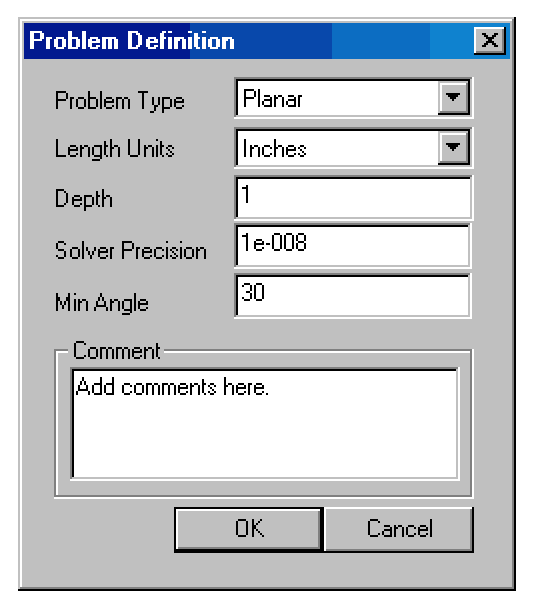
\includegraphics{belaman6.eps}}
\caption{Problem Definition dialog.}
\label{fig6}
\end{figure}

The first selection is the \texttt{Problem Type} drop list. This
drop box allows the user to choose from a 2-D planar problem (the
\texttt{Planar} selection), or an axisymmetric problem (the
\texttt{Axisymmetric} selection).





Next is the \texttt{Length Units} drop list. This box identifies
what unit is associated with the dimensions prescribed in the
model's geometry. Currently, the program supports inches,
millimeters, centimeters, meters, mils, and $\mu $meters.





The first edit box is the \texttt{Depth} specification. If a Planar
problem is selected, this edit box becomes enabled. This value is
the length of the geometry in the ``into the page'' direction. This
value is used for scaling integral results in the post processor
(e.g. force, inductance, etc.) to the appropriate length. The units
of the Depth selection are the same as the selected length units.

The second edit box is the \texttt{Solver Precision} edit box. The
number in this edit box specifies the stopping criteria for the
linear solver. The linear algebra problem could be represented by:

\begin{equation}
M x = b
\end{equation}

\noindent
where $M$ is a square matrix, $b$ is a vector, and $x$ is a vector of
unknowns to be determined. The solver precision value determines the maximum
allowable value for $\vert \vert b - Mx\vert \vert / \vert \vert b\vert
\vert $. The default value is $10^{ - 8}$.

The third edit box is labeled {\tt Min Angle}.  The entry in this box is used as a
constraint in the Triangle meshing program.  Triangle adds points to the mesh to
ensure that no angles smaller than the specified angle occur. If the minimum angle
is 20.7 degrees or smaller, the triangulation algorithm is theoretically guaranteed to
terminate (assuming infinite precision arithmetic -- Triangle may
fail to terminate if you run out of precision).  In practice, the
algorithm often succeeds for minimum angles up to 33.8 degrees.
For highly refined meshes, however, it may be necessary to reduce
the minimum angle to well below 20 to avoid problems associated
with insufficient floating-point precision.  The edit box will accept
values between 1 and 33.8 degrees.

Lastly, there is an optional \texttt{Comment} edit box. The user
can enter in a few lines of text that give a brief description of
the problem that is being solved. This is useful if the user is
running several small variations on a given geometry. The comment
can then be used to identify the relevant features for a particular
geometry.

\subsection{Definition of Properties}

To make a solvable problem definition, the user must identify boundary
conditions, block materials properties, and so on. The different types of
properties defined for a given problem are defined via the
\texttt{Properties} selection off of the main menu.

When the \texttt{Properties} selection is chosen, a drop menu
appears that has selections for Materials, Boundary, Point, and
Conductors. When any one of these selections is chosen, the dialog
pictured in Figure~\ref{fig7} appears.

\begin{figure}[htbp]
\centerline{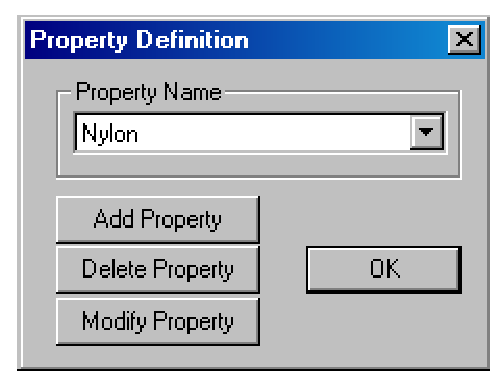
\includegraphics{belaman7.eps}}
\caption{Property Definition dialog box.}
\label{fig7}
\end{figure}




This dialog is the manager for a particular type of properties. All
currently defined properties are displayed in the \texttt{Property
Name} drop list at the top of the dialog. At the beginning of a new
model definition, the box will be blank, since no properties have
yet been defined. Pushing the \texttt{Add Property} button allows
the user to define a new property type. The \texttt{Delete
Property} button removes the definition of the property currently
in view in the \texttt{Property Name} box. The \texttt{Modify
Property} button allows the user to view and edit the property
currently selected in the \texttt{Property Name} box. Specifics for
defining the various property types are addressed in the
following subsections.

\subsubsection{Point Properties}

If a new point property is added or an existing point property modified, the
\texttt{Nodal Property} dialog box appears. This dialog box is pictured in
Figure~\ref{fig8}.

\begin{figure}[htbp]
\centerline{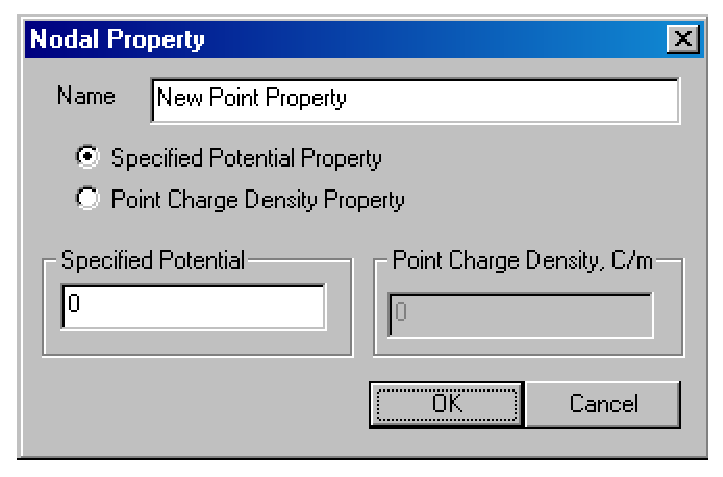
\includegraphics{belaman8.eps}}
\caption{Nodal Property dialog.}
\label{fig8}
\end{figure}




The first selection is the \texttt{Name} edit box. The default name
is ``New Point Property,'' but this name should be changed to
something that describes the property that you are defining.





Next are edit boxes for defining the voltage at a given point, or
prescribing a point charge density at a given point. The type of point
property is chosen via the radio buttons, and the value is entered in the
enabled edit box.

\subsubsection{Boundary Properties}





The \texttt{Boundary Property} dialog box is used to specify the
properties of line segments or arc segments that are to be
boundaries of the solution domain. When a new boundary property is
added or an existing property modified, the \texttt{Boundary
Property} dialog pictured in Figure~\ref{fig9} appears.

\begin{figure}[htbp]
\centerline{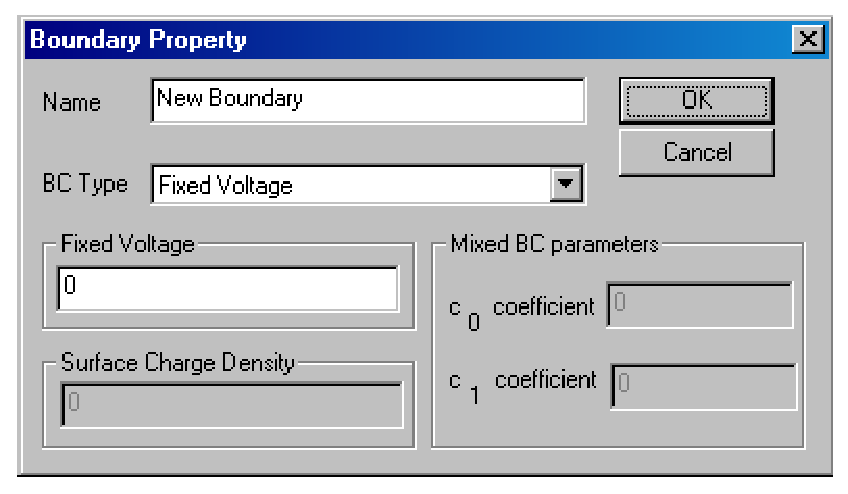
\includegraphics{belaman9.eps}}
\caption{Boundary Property dialog.}
\label{fig9}
\end{figure}

The first selection in the dialog is the \texttt{Name} of the
property. The default name is ``New Boundary,'' but you should
change this name to something more descriptive of the boundary that
is being defined.

The next selection is the \texttt{BC Type} drop list. This
specifies the boundary condition type. Currently, FEMM electrostatics problems 
support the following types of boundaries:

\texttt{Fixed Voltage} With this type of boundary condition, potential $V$ is
set to a prescribed along a given boundary

\texttt{Mixed} This denotes a boundary condition of the form:

\begin{equation}
\label{eq7}
\varepsilon _r \varepsilon _o \frac{\partial V}{\partial n} + c_o V + c_1 =
0
\end{equation}

The parameters for this class of boundary condition are specified in the
\texttt{Mixed BC parameters} box in the dialog. By the choice of
coefficients, this boundary condition can either be a Robin or a Neumann
boundary condition. By carefully selecting the $c_0 $ coefficient and
specifying $c_1 = 0$, this boundary condition can be applied to the outer
boundary of your geometry to approximate an unbounded solution region. For
more information on open boundary problems, refer to the Appendix.

\texttt{Surface Charge Density }This selection is used to apply
distributions of line charge to segments or arc segments in the problem.
Unlike all of the other boundary conditions, this BC type is often used on
internal boundaries between materials or on isolated segments. Typically,
other BCs are only used on exterior boundaries.

\texttt{Periodic} This type of boundary condition is applied to either two
segments or two arcs to force the potential to be identical along each
boundary. This sort of boundary is useful in exploiting the symmetry
inherent in some problems to reduce the size of the domain which must be
modeled. The domain merely needs to be periodic, as opposed to obeying more
restrictive $V = 0$ or $\partial V / \partial n = 0$ line of symmetry
conditions. Another useful application of periodic boundary conditions is
for the modeling of ``open boundary'' problems, as discussed in Appendix~3.
Often, a periodic boundary is made up of several different line or arc
segments. A different periodic condition must be defined for each section of
the boundary, since each periodic BC can only be applied to a line or arc
and a corresponding line or arc on the remote periodic boundary.

\texttt{Antiperiodic} The antiperiodic boundary condition is
applied in a similar way as the periodic boundary condition, but
its effect is to force two boundaries to be the negative of one
another. This type of boundary is also typically used to reduce the
domain which must be modeled, e.g. so that an electric machine
might be modeled for the purposes of a finite element analysis with
just one pole.

\subsubsection{Materials Properties}

The \texttt{Block Property} dialog box is used to specify the
properties to be associated with block labels. The properties
specified in this dialog have to do with the material of which the
block is composed. When a new material property is added or an
existing property modified, the
\texttt{Block Property} dialog pictured in Figure~\ref{fig10} appears.

\begin{figure}[htbp]
\centerline{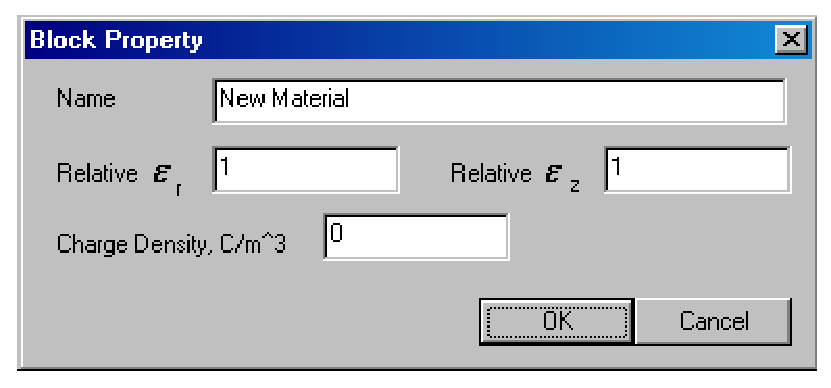
\includegraphics{belaman10.eps}}
\caption{Block Property dialog.}
\label{fig10}
\end{figure}

As with Point and Boundary properties, the first step is to choose a
descriptive name for the material that is being described. Enter it in the
\texttt{Name} edit box in lieu of ``New Material.''

Next, permittivity for the material needs to be specified. FEMM allows you
to specify different relative permittivities in the vertical and horizontal
directions (\textit{$\varepsilon $}$_{x}$ for the x- or horizontal direction, and \textit{$\varepsilon $}$_{y}$ for the y-
or vertical .

A volume charge density (\textit{$\rho $}) can also be prescribed by filling in the
appropriate box in the material properties dialog.


\subsubsection{Materials Library}

Since one kind of material might be needed in several different
models, FEMM has a built-in library of electrostatic Block Property definitions.
The user can access and maintain this library through the
\texttt{Properties $\vert $ Materials Library} selection off of the
main menu. When this option is selected, the
\texttt{Materials Library} dialog pictured in Figure~\ref{fig11} appears.

\begin{figure}[htbp]
\centerline{\includegraphics{bd_matlib.ps}}
\caption{Materials Library dialog}
\label{fig11}
\end{figure}

This dialog allow the user to exchange Block
Property definitions between the current model and the materials
library via a drag-and-drop interface.

A number of different options are available via a mouse button right-click
when the cursor is located on top of a material or folder. Materials can be edited
by double-clicking on the desired material.

Material from other material libraries or models can be imported by selecting the
``Import Materials'' option from the right-button menu that appears when the pointer
is over the root-level folder of either the Library or Model materials lists.

The materials library should be located in the same directory as
the femm executable files, under the filename \texttt{statlib.dat}.
If you move the materials library, femm will not be able to find
it.

\subsubsection{Conductor Properties}

The purpose of the conductor properties is mainly to allow the user to apply
constraints on the total amount of charge carried on a conductor.
Alternatively, conductors with a fixed voltage can be defined, and the
program will compute the total charge carried on the conductor during the
solution process.





For fixed voltages, one could alternatively apply a \texttt{Fixed
Voltage} boundary condition. However, applying a fixed voltage as a
conductor allows the user to group together several physically
disjoint surfaces into one conductor upon which the total net
charge is automatically computed.





The dialog for entering conductor properties is pictured in
Figure~\ref{fig12}.

\begin{figure}[htbp]
\centerline{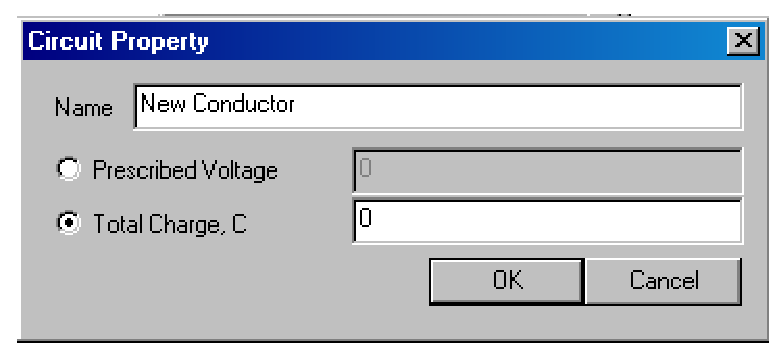
\includegraphics{belaman12.eps}}
\caption{Conductor Property dialog.}
\label{fig12}
\end{figure}

\subsection{Analysis Tasks}

Meshing the model, analyzing the model, and viewing the results are
most easily performed by the toolbar buttons pictured in
Figure~\ref{fig13}.

\begin{figure}[htbp]
\centerline{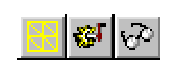
\includegraphics{belaman13.eps}}
\caption{Toolbar buttons for starting analysis tasks.}
\label{fig13}
\end{figure}

The first of these buttons (with the ``yellow mesh'' icon) runs the
mesh generator. The solver actually automatically calls the mesh
generator to make sure that the mesh is up to date, so you never
have to call the mesher from within femm. However, it is almost
always important to get a look at the mesh and see that it ``looks
right.'' When the mesh generation button is pressed, the mesher is
called. While the mesher is running, an entry labeled ``triangle''
will appear on the Windows taskbar. After the geometry is
triangulated, the finite element mesh is loaded into memory and
displayed underneath the defined nodes, segments, and block labels
as a set of yellow lines.

If you have a very large model, just keeping all of the mesh
information in core can take up a significant amount of memory. If
you are about to analyze a very large problem, it might be a good
idea to choose the \texttt{Mesh $\vert $ Purge Mesh} option off of
the main menu. When this option is selected, the mesh is removed
from memory, and the memory that it occupied is freed for other
uses.

The second button, with the ``hand-crank'' icon, executes the solver,
\texttt{Belasolv.exe}. Before Belasolve is actually run, the Triangle is
called to make sure the mesh is up to date. Then, Belasolve is called. When
Belasolve runs, it opens up a console window to display status information
to the user. However, Belasolve requires no user interaction while it is
running. When Belasolve is finished analyzing your problem, the console
window will disappear. The time that Belasolve requires is highly dependent
on the problem being solved. Solution times are typically on the order of 1
to 10 seconds, depending upon the size and complexity of the problem and the
speed of the machine analyzing the problem.

The ``big magnifying glass'' icon is used to run the postprocessor once the
analysis is finished.



%------------------------------------------------------------------------------------
\section{Electrostatics Postprocessor}


The the electrostaticss postprocessing functionality of femm is
used to view solutions generated by the {\tt belasolv} solver.  An
electrostatics postprocessor window can be opened either by loading
some previously run analyses via {\tt File|Open} on the main menu,
or by pressing the ``big magnifying glass'' icon from within a
preprocessor window to view a newly generated solution.
Electrostatics postprocessor data files stored on disk have the
{\tt .res} prefix.

Operation of the electrostatics postprocessor ({\em i.e.} modes, view manipulation) is
very similar to that of the magnetics postprocessor.  Refer to
Sections~\ref{tape} through~\ref{scissors} for this information.

\subsection{Contour Plot}

One of the most useful ways to get a subjective feel for a solution
is by plotting the eqipotentials of voltage. By default, a set of
19 equipotential lines are plotted when a solution is initially
loaded into the postprocessor. The number and type of equipotential
lines to be plotted can be altered using the Contours Plot icon in
the Graph Mode section of the toolbar (see Figure~\ref{fig17}). The
Contour Plot icon is the icon with the black contours.

\begin{figure}[htbp]
\centerline{\includegraphics{hplotbar.ps}}
\caption{Graph Mode toolbar buttons.}
\label{fig17}
\end{figure}




When this button is pressed, a dialog pops up, allowing the choice of the
number of contours.





In the contour plot dialog, a check box is also present titled ``Show stress
tensor mask''. If this box is checked, the contour lines associated with the
last Weighted Stress Tensor integration are also displayed, by default as
orange flux lines.

\subsection{Density Plot}

Density plots are also a useful way to get a quick feel for the
flux density in various parts of the model. By default, a flux
density plot is not displayed when the postprocessor first starts.
However, the plot can be displayed by pressing the middle button in
the Graph Mode section of the toolbar (see Figure~\ref{fig17}). A
dialog the pops up that allows the user to turn density plotting
on.

The user can select between density plots of Voltage (V) or the magnitude of
Electric Field Intensity (E) or Electric Flux Density (D). The field at each
point is classified into one of twenty contours distributed evenly between
either the minimum and maximum flux densities or user-specified bounds.

\subsection{Vector Plots}

A good way of getting a feel for the direction and magnitude of the
field is with plots of the field vectors. With this type of plot
arrows are plotted such that the direction of the arrow indicates
the direction of the field and the size of the arrow indicates the
magnitude of the field. The presence and appearance of this type of
plot can be controlled by pressing the ``arrows'' icon pictured in
Figure~\ref{fig17}.

\subsection{Line Plots}

When the postprocessor is in Contours Mode, various field values of
interest can be plotted along the defined contour. A plot of a
field value defined contour is performed by pressing the ``graphed
function'' icon in the Plot, Integration and Conductor Results group of toolbar
buttons, shown in Figure~\ref{fig18}.

\begin{figure}[htbp]
\centerline{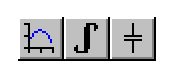
\includegraphics{belaman18.eps}}
\caption{Line Plot, Integration, and Conductor Results toolbar buttons.}
\label{fig18}
\end{figure}


When this button is pressed, the \texttt{X-Y Plot} dialog (see
Figure~\ref{fig19}) appears with a drop list containing the types
of line plots available. Choose the desired type of plot and press
``OK.''

\begin{figure}[htbp]
\centerline{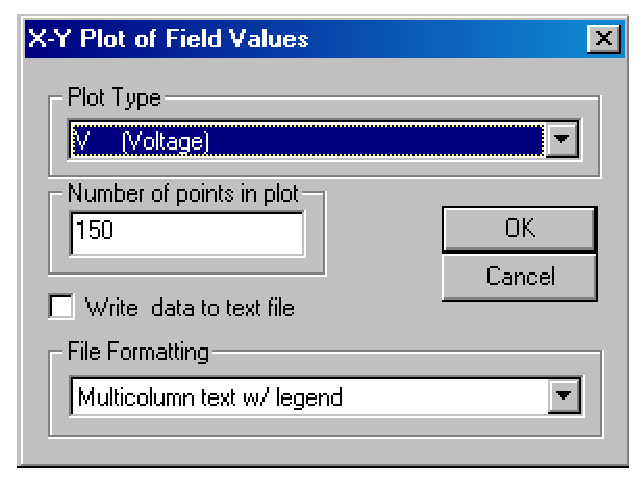
\includegraphics{belaman19.eps}}
\caption{X-Y Plot dialog.}
\label{fig19}
\end{figure}




After ``OK'' is pressed, the program computes the desired values
along the defined contour. These values are then plotted using the
\texttt{femmplot} program, which is called automatically to display
the plot.





By default, the \texttt{Write data to text file} box is not
checked. If the user selects this option, the file selection dialog
will appear and prompt for a filename to which to write the data.
The data is written in two-column text format. If \texttt{Write
data to text file} is selected, a femmplot window will not appear.





Currently, the type of line plots supported are: Potential along the
contour; Magnitude of the flux density along the contour; Component of flux
density normal to the contour; Component of flux density tangential to the
contour; Magnitude of the field intensity along the contour; Component of
field intensity normal to the contour; Component of field intensity
tangential to the contour;





In all of these plots, the direction of the normal is understood to
be as shown in Figure~\ref{fig20}. The tangential direction is
understood to be the direction in which the contour was defined.

\begin{figure}[htbp]
\centerline{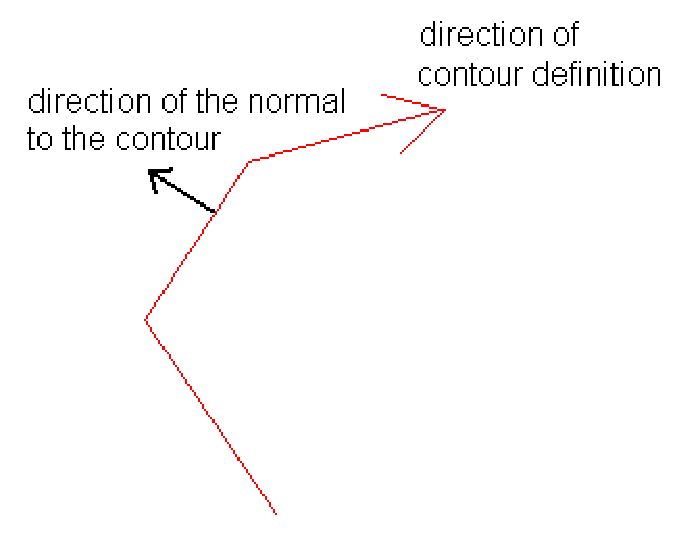
\includegraphics{belaman20.eps}}
\caption{When in doubt plots and integrals taken on this side of a contour.}
\label{fig20}
\end{figure}




In certain cases, the quantity to be plotted can be ambiguous. This
can occur, for example, if a plot of the tangential field intensity
is requested on a contour running along an interface between two
materials of differing permittivity. In this case, there is a
discontinuity in the tangential field intensity, and the value of
this quantity is different on each side of the interface. The
postprocessor resolves the conflict by always evaluating the plots
at a differentially small distance to the ``normal'' side of the
line. Therefore, by defining the same contour but reversing the
order in which the points are specified, plots of the quantity of
interest on each side of a boundary can be obtained.

\subsection{Line Integrals}

Once a contour has been specified in Contours mode, Line Integrals can be
performed along the specified contour. These integrals are performed by
evaluating a large number of points at evenly spaced along the contour and
integrating using a simple trapezoidal-type integration scheme.

To perform an integration, press the ``integral'' icon on the
toolbar (as shown in Figure~0). A small dialog will appear with a
drop list. Choose the desired integral from the drop list and press
\texttt{OK}. The amount of time required to perform the integral
will be virtually instantaneous for some types of integrals;
however, some types may require several seconds to evaluate. When
the evaluation of the integral is completed, the answer appears on
the screen in a pop-up box.

The line integrals currently supported are:


\begin{itemize}


\item \texttt{E.t }This integral returns the voltage drop along the defined
contour

\item \texttt{D.n}. This integral returns the total electrix flux passing through
a volume defined by extruding or sweeping the defined contour. If this
integral is performed over a closed contour, the resulting quantity is equal
to the charge contained inside the contour.

\item \texttt{Contour Length/Area}. This integral returns the length of the
defined contour in meters, as well as the area of the extruded or swept
volume associated with the defined contour.

\item \texttt{Force from stress tensor}. This integral totals the force produced
on the contour derived from Maxwell's stress tensor. Deriving
meaningful force results requires some care in the choice of
integration path; refer to Section~\ref{forcetorquesection} for a
detailed discussion of force and torque calculation.

\item \texttt{Torque from stress tensor}. This selection integrates the torque
about the point (0,0) inferred from Maxwell's stress tensor. Again,
some guidelines must be followed to get accurate torque results.

\end{itemize}



\subsection{Block Integrals}

To select the regions over which a block integral is to be performed,
left-click with the mouse in the desired region. The selected region will
appear highlighted in green. For some block integrals ($i.e.$ weighted stress
tensor force and torque), one desires to select a conductor composed of
lines and points, rather than a block. In this case, the desired conductor
can be selected by clicking on it with the right mouse button. The selected
conductor will appear in red.

To perform an integration, press the ``integral'' icon on the
toolbar (as shown in Figure~\ref{fig18}), and a dialog will appear
with a drop list. Choose the desired integral from the drop list
and press \texttt{OK}. The integral is then performed by
analytically integrating the specified kernel over each element in
the defined region, and summing the results for all elements.
Volume integrals may take several seconds to evaluate, especially
on dense meshes. Be patient. When the evaluation of the integral is
completed, the answer appears on the screen in a pop-up box.





The block integrals currently supported are:


\begin{itemize}


\item \texttt{Stored Energy }This selection calculates the energy stored in the
electric field in the specified region by integrating ($\frac{1}{2}
D \cdot E$) over the selected area.

\item \texttt{Block cross-section area}

\item \texttt{Block volume}

\item \texttt{Average D over volume}

\item \texttt{Average E over volume}

\item \texttt{Force via Weighted Stress Tensor }The Weighted Stress Tensor block
integrals automatically compute a weighting function over the
finite element mesh that allows all possible air elements to
contribute to the stress tensor integration. This approach is
similar to the weighted stress tensor approach described in
\cite{mcfee} and/or \cite{henforce}. To compute the force on a region or
set of regions, the user selects the blocks upon which force result
is desired and selects the \texttt{Force via Weighted Stress
Tensor} integral. The program then computes the weighting function
by solving an additional Laplace equation over the air surrounding
the blocks upon which the force is to be computed. It may take a
few seconds to compute the weighting function--progress is be
indicated by a progress bar that is displayed while the weighting
function is being computed. The stress tensor is then evaluated as
a volume integration, and the results are displayed. The results
are typically more accurate than the Maxwell Stress Tensor line
integral, since in some sense, all possible contours have been
averaged to yield the Weighted Stress Tensor force result.


If the user is interested in the contours along which the integral was
performed, the "stress tensor mask" box can be checked in the contour plot
dialog. A set of orange (by default) lines will be displayed that.

\item \texttt{Torque via Weighted Stress Tensor} This integral is torque version
of the \texttt{Force via Weighted Stress Tensor} integral. Instead
of force, torque about (0,0) is computed using the same weighting
function approach.
\end{itemize}


\subsection{Force/Torque Calculation} \label{forcetorquesection}

Often, the calculation of electrostatic and torques is a goal of
finite element analysis. This section discusses some of the
different methods of deducing electrostatic forces and torques.

\subsubsection{Weighted Stress Tensor Volume Integral}

This volume integral greatly simplifies the computation of forces and
torques. Merely select the blocks or conductors upon which force or torque
are to be computed and evaluate the integral. No particular ``art'' is
required in getting good force or torque results (as opposed to the Stress
tensor line integral), although results tend to be more accurate with finer
meshing around the region upon which the force or torque is to be computed.

One limitation of the Weighted Stress Tensor integral is that the regions
upon which the force is being computed must be entirely surrounded by air
and/or abutting a boundary. In cases in which the desired region abuts a
non-air region, force results may be deduced from differentiation of stored
electric field energy.

\subsubsection{Maxwell Stress Tensor Line Integral}

Generally, you should not use the Stress Tensor line integral to compute
forces and torques if it can be avoided (i.e. use the volume integral
version instead). The indiscriminate use Maxwell's Stress Tensor can result
in bad predictions forces and torques.

Maxwell's stress tensor prescribes a force per unit area produced by the
electric field on a surface. The differential force produced is:

\begin{equation}
\label{eq8}
dF = \frac{1}{2}\left( {D\left( {E \cdot n} \right) + E\left( {D \cdot n}
\right) - \left( {D \cdot E} \right)n} \right)
\end{equation}

\noindent
where $n$ denotes the direction normal to the surface at the point of interest.
The net force on an object is obtained by creating a surface totally
enclosing the object of interest and integrating the stress over that
surface.

For best results, never integrate the stress tensor along an interface
between materials. Always define the integration contour as a closed path
around the object of interest with the contour displaced several elements
(at least two elements) away from any interfaces or boundaries.

Always use as fine a mesh as possible in problems where force results are
desired. A good way to proceed in finding a mesh that is ``dense enough'' is
to solve the problem on progressively finer meshes, evaluating the force on
each mesh. By comparing the results from different mesh densities, you can
get and idea of the level of accuracy (by looking at what digits in the
answer that change between various mesh densities). You then pick the
smallest mesh density that gives convergence to the desired digit of
accuracy.

For torque computations, all the same rules apply as for force computations
(i.e. define integration contours away from boundaries and interfaces, and
use a dense mesh).

\subsection{Conductor Results}

If conductor properties are used to specify the excitation, a
useful byproduct is ready access to the voltage and charge on the
conductor. To view the conductor results, either press the ``Conductor Results''
toolbar button pictured in Figure~\ref{fig18} or select \texttt{View$\vert
$Conductor Props} off of the postprocessor main menu. A dialog, as
pictured in Figure~\ref{fig21} will appear. There is a drop list on the
dialog, from which the user selects the conductor for which results
are desired. When a conductor is selected, the voltage and charge
associated with that conductor are displayed.

\begin{figure}[htbp]
\centerline{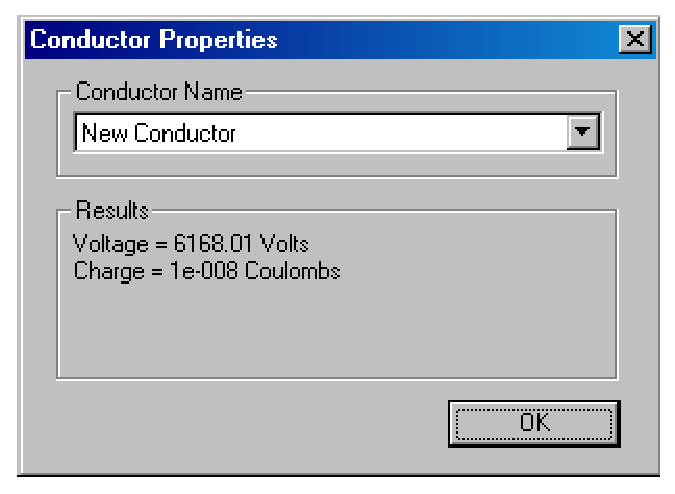
\includegraphics{belaman21.eps}}
\caption{Conductor results dialog.}
\label{fig21}
\end{figure}


%-----------------------------------------------------------------------------------
% Heat Flow Stuff

%------------------------------------------------------------------------------------
\section{Heat Flow Preprocessor}

The preprocessor is used for drawing the problems geometry, defining
materials, and defining boundary conditions. The process of construction of heat
flow problems is mechanically nearly identical to the construction of
magnetics problems--refer to Sections~\ref{pencil} through~\ref{coffee} for
an overview of the FEMM editing and problem creation commands. This section
considers those parts of problem definition that are unique to heat flow problems.

\subsection{Problem Definition}

The definition of problem type is specified by choosing the
\texttt{Problem} selection off of the main menu. Selecting this
option brings up the Problem Definition dialog, shown in
Figure~\ref{hfig5}.

\begin{figure}[htbp]
\centerline{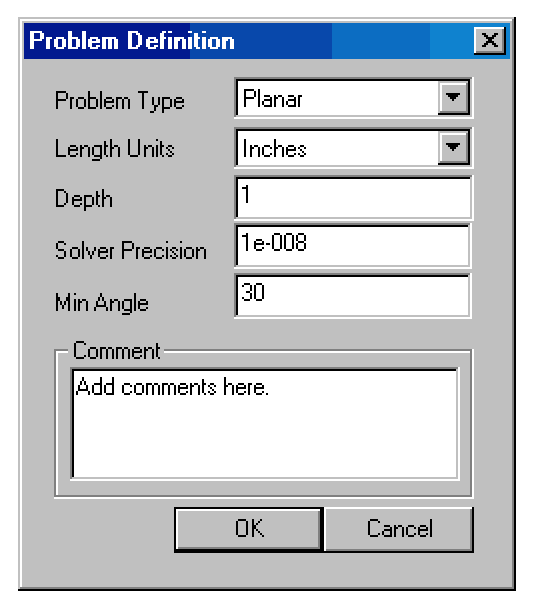
\includegraphics{belaman6.eps}}
\caption{Problem Definition dialog.}
\label{hfig5}
\end{figure}

The first selection is the \texttt{Problem Type} drop list. This
drop box allows the user to choose from a 2-D planar problem (the
\texttt{Planar} selection), or an axisymmetric problem (the
\texttt{Axisymmetric} selection).





Next is the \texttt{Length Units} drop list. This box identifies
what unit is associated with the dimensions prescribed in the
model's geometry. Currently, the program supports inches,
millimeters, centimeters, meters, mils, and $\mu $meters.





The first edit box is the \texttt{Depth} specification. If a Planar
problem is selected, this edit box becomes enabled. This value is
the length of the geometry in the ``into the page'' direction. This
value is used for scaling integral results in the post processor
(e.g. force, inductance, etc.) to the appropriate length. The units
of the Depth selection are the same as the selected length units.

The second edit box is the \texttt{Solver Precision} edit box. The
number in this edit box specifies the stopping criteria for the
linear solver. The linear algebra problem could be represented by:

\begin{equation}
M x = b
\end{equation}

\noindent
where $M$ is a square matrix, $b$ is a vector, and $x$ is a vector of
unknowns to be determined. The solver precision value determines the maximum
allowable value for $\vert \vert b - Mx\vert \vert / \vert \vert b\vert
\vert $. The default value is $10^{ - 8}$.

The third edit box is labeled {\tt Min Angle}.  The entry in this box is used as a
constraint in the Triangle meshing program.  Triangle adds points to the mesh to
ensure that no angles smaller than the specified angle occur. If the minimum angle
is 20.7 degrees or smaller, the triangulation algorithm is theoretically guaranteed to
terminate (assuming infinite precision arithmetic -- Triangle may
fail to terminate if you run out of precision).  In practice, the
algorithm often succeeds for minimum angles up to 33.8 degrees.
For highly refined meshes, however, it may be necessary to reduce
the minimum angle to well below 20 to avoid problems associated
with insufficient floating-point precision.  The edit box will accept
values between 1 and 33.8 degrees.

Lastly, there is an optional \texttt{Comment} edit box. The user
can enter in a few lines of text that give a brief description of
the problem that is being solved. This is useful if the user is
running several small variations on a given geometry. The comment
can then be used to identify the relevant features for a particular
geometry.

\subsection{Definition of Properties}

To make a solvable problem definition, the user must identify boundary
conditions, block materials properties, and so on. The different types of
properties defined for a given problem are defined via the
\texttt{Properties} selection off of the main menu.

When the \texttt{Properties} selection is chosen, a drop menu
appears that has selections for Materials, Boundary, Point, and
Conductors. When any one of these selections is chosen, the dialog
pictured in Figure~\ref{hfig7} appears.

\begin{figure}[htbp]
\centerline{\includegraphics{hpropdef.ps}}
\caption{Property Definition dialog box.}
\label{hfig7}
\end{figure}




This dialog is the manager for a particular type of properties. All
currently defined properties are displayed in the \texttt{Property
Name} drop list at the top of the dialog. At the beginning of a new
model definition, the box will be blank, since no properties have
yet been defined. Pushing the \texttt{Add Property} button allows
the user to define a new property type. The \texttt{Delete
Property} button removes the definition of the property currently
in view in the \texttt{Property Name} box. The \texttt{Modify
Property} button allows the user to view and edit the property
currently selected in the \texttt{Property Name} box. Specifics for
defining the various property types are addressed in the
following subsections.

\subsubsection{Point Properties}

If a new point property is added or an existing point property modified, the
\texttt{Nodal Property} dialog box appears. This dialog box is pictured in
Figure~\ref{hfig8}.

\begin{figure}[htbp]
\centerline{\includegraphics{hnodeprop.ps}}
\caption{Nodal Property dialog.}
\label{hfig8}
\end{figure}

The first selection is the \texttt{Name} edit box. The default name
is {\tt New Point Property}, but this name should be changed to
something that describes the property that you are defining.

Next are edit boxes for defining the temperature at a given point, or
prescribing a heat generation at a given point. The type of point
property is chosen via the radio buttons, and the value is entered in the
enabled edit box.

\subsubsection{Boundary Properties}

The \texttt{Boundary Property} dialog box is used to specify the
properties of line segments or arc segments that are to be
boundaries of the solution domain. When a new boundary property is
added or an existing property modified, the \texttt{Boundary
Property} dialog pictured in Figure~\ref{hfig9} appears.

\begin{figure}[htbp]
\centerline{\includegraphics{hbdryprop.ps}}
\caption{Boundary Property dialog.}
\label{hfig9}
\end{figure}

The first selection in the dialog is the \texttt{Name} of the
property. The default name is {\tt New Boundary}, but you should
change this name to something more descriptive of the boundary that
is being defined.

The next selection is the \texttt{BC Type} drop list. This
specifies the boundary condition type. Currently, FEMM heat flow problems
support the following types of boundaries: Fixed Temperature, Heat Flux, Convection,
Radiation, Periodic, and Antiperiodic. These boundary conditions are
described in detail in Section~\ref{bcsection}.

\subsubsection{Materials Properties}

The \texttt{Block Property} dialog box is used to specify the
properties to be associated with block labels. The properties
specified in this dialog have to do with the material of which the
block is composed. When a new material property is added or an
existing property modified, the
\texttt{Block Property} dialog pictured in Figure~\ref{hfig10} appears.

\begin{figure}[htbp]
\centerline{\includegraphics{hblockprop.ps}}
\caption{Block Property dialog.}
\label{hfig10}
\end{figure}

As with Point and Boundary properties, the first step is to choose a
descriptive name for the material that is being described. Enter it in the
\texttt{Name} edit box in lieu of {\tt New Material}.

Next, the thermal conductivity for the material needs to be specified. There is a drop
list on the dialog that allows the user to select either a contant thermal conductivity
({\em i.e.} independent of temperature), or a thermal conductivity that is prescribed
as a function of temperature. If conductivity is selected, FEMM allows you
to specify different conductivities in the vertical and horizontal
directions (\textit{$\varepsilon $}$_{x}$ for the x- or horizontal direction, and \textit{$\varepsilon $}$_{y}$ for the y-
or vertical. If {\tt Thermal Conductivity Depends on Temperature} is selected, the 
{\tt Edit Nonlinear Thermal Conductivity Curve} becomes enabled.  Press the button
to enter temperature-conductivity pairs.  The program will interpolate linearly between 
the entered points.  If the program must extrapolate off the end of the defined curve,
conductivity takes the value of the nearest defined T-k point.

A volume heat generation can also be prescribed by filling in the
appropriate box in the material properties dialog.

\subsubsection{Materials Library}

Since one kind of material might be needed in several different
models, FEMM has a built-in library of thermal Block Property definitions.
The user can access and maintain this library through the
\texttt{Properties $\vert $ Materials Library} selection off of the
main menu. When this option is selected, the
\texttt{Materials Library} dialog pictured in Figure~\ref{hfig11} appears.

\begin{figure}[htbp]
\centerline{\includegraphics{hmatlib.ps}}
\caption{Materials Library dialog}
\label{hfig11}
\end{figure}

This dialog allow the user to exchange Block
Property definitions between the current model and the materials
library via a drag-and-drop interface.

A number of different options are available via a mouse button right-click
when the cursor is located on top of a material or folder. Materials can be edited
by double-clicking on the desired material.

Material from other material libraries or models can be imported by selecting the
``Import Materials'' option from the right-button menu that appears when the pointer
is over the root-level folder of either the Library or Model materials lists.

The materials library should be located in the same directory as
the FEMM executable files, under the filename \texttt{heatlib.dat}.
If you move the materials library, FEMM will not be able to find
it.

\subsubsection{Conductor Properties}

The purpose of the conductor properties is mainly to allow the user to apply
constraints on the total amount of heat flowing in and out of a surface.
Alternatively, conductors with a fixed temperature can be defined, and the
program will compute the total heat flow through the during the
solution process.

For fixed temperatures, one could alternatively apply a \texttt{Fixed
Temperature} boundary condition. However, applying a fixed temperature
as a conductor allows the user to group together several physically
disjoint surfaces into one conductor upon which the total heat flux 
is automatically computed.

The dialog for entering conductor properties is pictured in
Figure~\ref{hfig12}.

\begin{figure}[htbp]
\centerline{\includegraphics{hcircprop.ps}}
\caption{Conductor Property dialog.}
\label{hfig12}
\end{figure}

\subsection{Analysis Tasks}

Meshing the model, analyzing the model, and viewing the results are
most easily performed by the toolbar buttons pictured in
Figure~\ref{hfig13}.

\begin{figure}[htbp]
\centerline{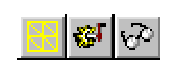
\includegraphics{belaman13.eps}}
\caption{Toolbar buttons for starting analysis tasks.}
\label{hfig13}
\end{figure}

The first of these buttons (with the ``yellow mesh'' icon) runs the
mesh generator. The solver actually automatically calls the mesh
generator to make sure that the mesh is up to date, so you never
have to call the mesher from within FEMM. However, it is almost
always important to get a look at the mesh and see that it ``looks
right.'' When the mesh generation button is pressed, the mesher is
called. While the mesher is running, an entry labeled ``triangle''
will appear on the Windows taskbar. After the geometry is
triangulated, the finite element mesh is loaded into memory and
displayed underneath the defined nodes, segments, and block labels
as a set of yellow lines.

If you have a very large model, just keeping all of the mesh
information in core can take up a significant amount of memory. If
you are about to analyze a very large problem, it might be a good
idea to choose the \texttt{Mesh $\vert $ Purge Mesh} option off of
the main menu. When this option is selected, the mesh is removed
from memory, and the memory that it occupied is freed for other
uses.

The second button, with the ``hand-crank'' icon, executes the solver,
\texttt{hsolv.exe}. Before hsolv is actually run, the Triangle is
called to make sure the mesh is up to date. Then, hsolv is called. When
hsolv runs, it opens up a console window to display status information
to the user. However, hsolv requires no user interaction while it is
running. When hsolv is finished analyzing your problem, the console
window will disappear. The time that hsolv requires is highly dependent
on the problem being solved. Solution times are typically on the order of 1
to 10 seconds, depending upon the size and complexity of the problem and the
speed of the machine analyzing the problem.

The ``big magnifying glass'' icon is used to run the postprocessor once the
analysis is finished.



%------------------------------------------------------------------------------------
\section{Heat Flow Postprocessor}

The the heat flow postprocessing functionality of FEMM is
used to view solutions generated by the {\tt hsolv} solver.  A heat flow
postprocessor window can be opened either by loading
some previously run analyses via {\tt File|Open} on the main menu,
or by pressing the ``big magnifying glass'' icon from within a
preprocessor window to view a newly generated solution.
Heat flow postprocessor data files stored on disk have the
{\tt .anh} prefix.

Operation of the heat flow postprocessor ({\em i.e.} modes, view manipulation) is
very similar to that of the magnetics postprocessor.  Refer to
Sections~\ref{tape} through~\ref{scissors} for this information.

\subsection{Contour Plot}

One of the most useful ways to get a subjective feel for a solution
is by plotting the eqipotentials of temperature. The number and type of equipotential
lines to be plotted can be altered using the Contours Plot icon in
the Graph Mode section of the toolbar (see Figure~\ref{hfig17}). The
Contour Plot icon is the icon with the black contours.

\begin{figure}[htbp]
\centerline{\includegraphics{hplotbar.ps}}
\caption{Graph Mode toolbar buttons.}
\label{hfig17}
\end{figure}

When this button is pressed, a dialog pops up, allowing the choice of the
number of contours.

\subsection{Density Plot}

Density plots are also a useful way to get a quick feel for the
temperature, flux density, etc., in various parts of the model. By default,
a density plot denoting temperature is displayed when the postprocessor first starts.
(This behavior can be changed via Edit|Preferences on the main menu).
However, the plot can be displayed by pressing the ``spectrum'' button in
the Graph Mode section of the toolbar (see Figure~\ref{hfig17}). A
dialog the pops up that allows the user to turn density plotting
on.

The user can select between density plots of temperature or the magnitude of
temperature gradient or heat flux density. The solution at each
point is classified into one of twenty contours distributed evenly between
either the minimum and maximum flux densities or user-specified bounds.

\subsection{Vector Plots}

A good way of getting a feel for the direction and magnitude of the
field is with plots of the field vectors. With this type of plot
arrows are plotted such that the direction of the arrow indicates
the direction of the field and the size of the arrow indicates the
magnitude of the field. The presence and appearance of this type of
plot can be controlled by pressing the ``arrows'' icon pictured in
Figure~\ref{hfig17}.

\subsection{Line Plots}

When the postprocessor is in Contours Mode, various field values of
interest can be plotted along the defined contour. A plot of a
field value defined contour is performed by pressing the ``graphed
function'' icon in the Plot, Integration and Conductor Results group of toolbar
buttons, shown in Figure~\ref{hfig18}.

\begin{figure}[htbp]
\centerline{\includegraphics{hresbar.ps}}
\caption{Line Plot, Integration, and Conductor Results toolbar buttons.}
\label{hfig18}
\end{figure}

When this button is pressed, the \texttt{X-Y Plot} dialog (see
Figure~\ref{hfig19}) appears with a drop list containing the types
of line plots available. Choose the desired type of plot and press
``OK.''

\begin{figure}[htbp]
\centerline{\includegraphics{hpltdlg.ps}}
\caption{X-Y Plot dialog.}
\label{hfig19}
\end{figure}

After ``OK'' is pressed, the program computes the desired values
along the defined contour. When the computation is finished, a window
will appear with a plot of the selected quantity.

By default, the \texttt{Write data to text file} box is not
checked. If the user selects this option, the file selection dialog
will appear and prompt for a filename to which to write the data.
The data is written in two-column text format. If \texttt{Write
data to text file} is selected, a plot window will not appear.

Currently, the type of line plots supported are: Temperature along the
contour; Magnitude of the heat flux density along the contour; Component of heat flux
density normal to the contour; Component of heat flux density tangential to the
contour; Magnitude of the temperature gradient along the contour; Component of
temperature gradient normal to the contour; Component of temperature gradient
tangential to the contour;

In all of these plots, the direction of the normal is understood to
be as shown in Figure~\ref{hfig20}. The tangential direction is
understood to be the direction in which the contour was defined.

\begin{figure}[htbp]
\centerline{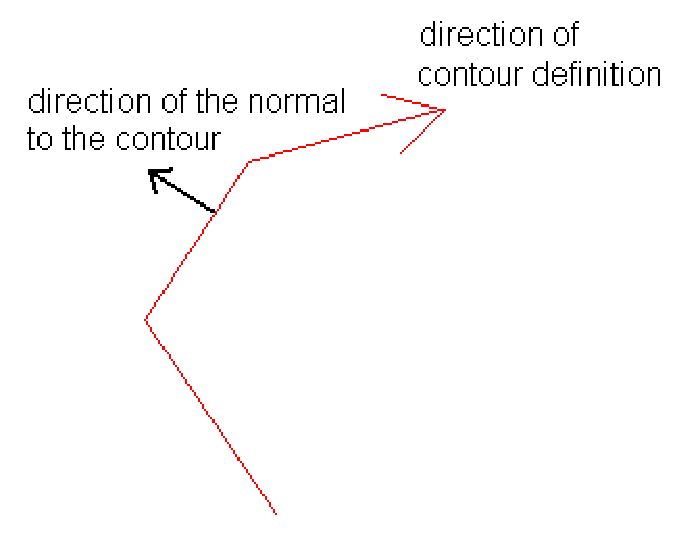
\includegraphics{belaman20.eps}}
\caption{When in doubt plots and integrals taken on this side of a contour.}
\label{hfig20}
\end{figure}




In certain cases, the quantity to be plotted can be ambiguous. This
can occur, for example, if a plot of the tangential field intensity
is requested on a contour running along an interface between two
materials of differing permittivity. In this case, there is a
discontinuity in the tangential field intensity, and the value of
this quantity is different on each side of the interface. The
postprocessor resolves the conflict by always evaluating the plots
at a differentially small distance to the ``normal'' side of the
line. Therefore, by defining the same contour but reversing the
order in which the points are specified, plots of the quantity of
interest on each side of a boundary can be obtained.

\subsection{Line Integrals}

Once a contour has been specified in Contours mode, Line Integrals can be
performed along the specified contour. These integrals are performed by
evaluating a large number of points at evenly spaced along the contour and
integrating using a simple trapezoidal-type integration scheme.

To perform an integration, press the ``integral'' icon on the
toolbar (as shown in Figure~0). A small dialog will appear with a
drop list. Choose the desired integral from the drop list and press
\texttt{OK}. The amount of time required to perform the integral
will be virtually instantaneous for some types of integrals;
however, some types may require several seconds to evaluate. When
the evaluation of the integral is completed, the answer appears on
the screen in a pop-up box.

The line integrals currently supported are:


\begin{itemize}


\item \texttt{Temperature Difference (G.t)}. This integral returns the 
temperature difference between the ends of the contour

\item \texttt{Heat Flux (F.n)}. This integral returns the total heat flux passing through
a volume defined by extruding or sweeping the defined contour.

\item \texttt{Contour length \& area}. The length of the contour, and the area formed by
extruding the contour.

\item \texttt{Average temperature}. The average temperature along the line.
\end{itemize}



\subsection{Block Integrals}

To select the regions over which a block integral is to be performed,
left-click with the mouse in the desired region. The selected region will
appear highlighted in green.

To perform an integration, press the ``integral'' icon on the
toolbar (as shown in Figure~\ref{hfig18}), and a dialog will appear
with a drop list. Choose the desired integral from the drop list
and press \texttt{OK}. The integral is then performed by
analytically integrating the specified kernel over each element in
the defined region, and summing the results for all elements.
Volume integrals may take several seconds to evaluate, especially
on dense meshes. Be patient. When the evaluation of the integral is
completed, the answer appears on the screen in a pop-up box.

The block integrals currently supported are:

\begin{itemize}

\item \texttt{Average temperature over volume}

\item \texttt{Block cross-section area}

\item \texttt{Block volume}

\item \texttt{Average F over volume}

\item \texttt{Average G over volume}

\end{itemize}

\subsection{Conductor Results}

If conductor properties are used to specify the excitation, a
useful byproduct is ready access to the temperature of and heat flux through the
conductor. To view the conductor results, either press the ``Conductor Results''
toolbar button pictured in Figure~\ref{hfig18} or select \texttt{View$\vert
$Conductor Props} off of the postprocessor main menu. A dialog, as
pictured in Figure~\ref{hfig21} will appear. There is a drop list on the
dialog, from which the user selects the conductor for which results
are desired. When a conductor is selected, the temperature and heat flux
associated with that conductor are displayed.

\begin{figure}[htbp]
\centerline{\includegraphics{hcircres.ps}}
\caption{Conductor results dialog.}
\label{hfig21}
\end{figure}



%-----------------------------------------------------------------------------------
% Current Flow Stuff

%------------------------------------------------------------------------------------
\section{Current Flow Preprocessor}

The preprocessor is used for drawing the problems geometry, defining
materials, and defining boundary conditions. The process of construction of current
flow problems is mechanically nearly identical to the construction of
magnetics problems--refer to Sections~\ref{pencil} through~\ref{coffee} for
an overview of the FEMM editing and problem creation commands. This section
considers those parts of problem definition that are unique to current flow problems.

\subsection{Problem Definition}

The definition of problem type is specified by choosing the
\texttt{Problem} selection off of the main menu. Selecting this
option brings up the Problem Definition dialog, shown in
Figure~\ref{cfig5}.

\begin{figure}[htbp]
\centerline{\includegraphics{cd1.ps}}
\caption{Problem Definition dialog.}
\label{cfig5}
\end{figure}

The first selection is the \texttt{Problem Type} drop list. This
drop box allows the user to choose from a 2-D planar problem (the
\texttt{Planar} selection), or an axisymmetric problem (the
\texttt{Axisymmetric} selection).

Next is the \texttt{Length Units} drop list. This box identifies
what unit is associated with the dimensions prescribed in the
model's geometry. Currently, the program supports inches,
millimeters, centimeters, meters, mils, and $\mu $meters.

The first edit box, {\tt Frequency, Hz}, denotes the frequency at 
which the problem is to be analyzed. 

The second edit box is the \texttt{Depth} specification. If a Planar
problem is selected, this edit box becomes enabled. This value is
the length of the geometry in the ``into the page'' direction. This
value is used for scaling integral results in the post processor
(e.g. force, inductance, etc.) to the appropriate length. The units
of the Depth selection are the same as the selected length units.

The second edit box is the \texttt{Solver Precision} edit box. The
number in this edit box specifies the stopping criteria for the
linear solver. The linear algebra problem could be represented by:

\begin{equation}
M x = b
\end{equation}

\noindent
where $M$ is a square matrix, $b$ is a vector, and $x$ is a vector of
unknowns to be determined. The solver precision value determines the maximum
allowable value for $\vert \vert b - Mx\vert \vert / \vert \vert b\vert
\vert $. The default value is $10^{ - 8}$.

The third edit box is labeled {\tt Min Angle}.  The entry in this box is used as a
constraint in the Triangle meshing program.  Triangle adds points to the mesh to
ensure that no angles smaller than the specified angle occur. If the minimum angle
is 20.7 degrees or smaller, the triangulation algorithm is theoretically guaranteed to
terminate (assuming infinite precision arithmetic -- Triangle may
fail to terminate if you run out of precision).  In practice, the
algorithm often succeeds for minimum angles up to 33.8 degrees.
For highly refined meshes, however, it may be necessary to reduce
the minimum angle to well below 20 to avoid problems associated
with insufficient floating-point precision.  The edit box will accept
values between 1 and 33.8 degrees.

Lastly, there is an optional \texttt{Comment} edit box. The user
can enter in a few lines of text that give a brief description of
the problem that is being solved. This is useful if the user is
running several small variations on a given geometry. The comment
can then be used to identify the relevant features for a particular
geometry.

\subsection{Definition of Properties}

To make a solvable problem definition, the user must identify boundary
conditions, block materials properties, and so on. The different types of
properties defined for a given problem are defined via the
\texttt{Properties} selection off of the main menu.

When the \texttt{Properties} selection is chosen, a drop menu
appears that has selections for Materials, Boundary, Point, and
Conductors. When any one of these selections is chosen, the dialog
pictured in Figure~\ref{cfig7} appears.

\begin{figure}[htbp]
\centerline{\includegraphics{hpropdef.ps}}
\caption{Property Definition dialog box.}
\label{cfig7}
\end{figure}

This dialog is the manager for a particular type of properties. All
currently defined properties are displayed in the \texttt{Property
Name} drop list at the top of the dialog. At the beginning of a new
model definition, the box will be blank, since no properties have
yet been defined. Pushing the \texttt{Add Property} button allows
the user to define a new property type. The \texttt{Delete
Property} button removes the definition of the property currently
in view in the \texttt{Property Name} box. The \texttt{Modify
Property} button allows the user to view and edit the property
currently selected in the \texttt{Property Name} box. Specifics for
defining the various property types are addressed in the
following subsections.

\subsubsection{Point Properties}

If a new point property is added or an existing point property modified, the
\texttt{Nodal Property} dialog box appears. This dialog box is pictured in
Figure~\ref{cfig8}.

\begin{figure}[htbp]
\centerline{\includegraphics{cd2.ps}}
\caption{Nodal Property dialog.}
\label{cfig8}
\end{figure}

The first selection is the \texttt{Name} edit box. The default name
is {\tt New Point Property}, but this name should be changed to
something that describes the property that you are defining.

Next are edit boxes for defining the voltage at a given point, or
prescribing a current generation at a given point. The type of point
property is chosen via the radio buttons, and the value is entered in the
enabled edit box.

\subsubsection{Boundary Properties}

The \texttt{Boundary Property} dialog box is used to specify the
properties of line segments or arc segments that are to be
boundaries of the solution domain. When a new boundary property is
added or an existing property modified, the \texttt{Boundary
Property} dialog pictured in Figure~\ref{cfig9} appears.

\begin{figure}[htbp]
\centerline{\includegraphics{cd3.ps}}
\caption{Boundary Property dialog.}
\label{cfig9}
\end{figure}

The first selection in the dialog is the \texttt{Name} of the
property. The default name is {\tt New Boundary}, but you should
change this name to something more descriptive of the boundary that
is being defined.

The next selection is the \texttt{BC Type} drop list. This
specifies the boundary condition type. Currently, FEMM supports the
following types of boundaries: Fixed Voltage, Mixed, Prescribed surface current density,
Periodic, and Antiperiodic. These boundary conditions are
described in detail in Section~\ref{bcsection}.

\subsubsection{Materials Properties}

The \texttt{Block Property} dialog box is used to specify the
properties to be associated with block labels. The properties
specified in this dialog have to do with the material of which the
block is composed. When a new material property is added or an
existing property modified, the
\texttt{Block Property} dialog pictured in Figure~\ref{cfig10} appears.

\begin{figure}[htbp]
\centerline{\includegraphics{cd4.ps}}
\caption{Block Property dialog.}
\label{cfig10}
\end{figure}

As with Point and Boundary properties, the first step is to choose a
descriptive name for the material that is being described. Enter it in the
\texttt{Name} edit box in lieu of {\tt New Material}.

%Electrical Conductivity
%Relative Electrical Permittivity
%Loss Tangent

Next, electrical conductivitiy for the material needs to be specified. FEMM allows you
to specify different electrical conductivities in the vertical and horizontal
directions (\textit{$\sigma$}$_{x}$ for the x- or horizontal direction, and \textit{$\sigma$}$_{y}$ for the y-
or vertical direction.

The next pair of boxes represents the relative electrical permittivity for the material. Similar to the
electrical conducitvity, textit{$\varepsilon $}$_{x}$ represents permittivity in the x- or horizontal direction,
and \textit{$\varepsilon $}$_{y}$ for the y- or vertical direction.  If the material is
a lossy dielectric, this value is considered to be the amplitude of complex permittivity.

%        if( _strnicmp(q,"<ltx>",5)==0){
%           v=StripKey(s);
%           double lt;
%           sscanf(v,"%lf",&lt);
%           lt=-atan(lt);
%           MProp.ex=MProp.ex*exp(I*lt);
%           q[0]=NULL;
%        }
%
%        if( _strnicmp(q,"<lty>",5)==0){
%           v=StripKey(s);
%           double lt;
%           sscanf(v,"%lf",&lt);
%           lt=-atan(lt);
%           MProp.ey=MProp.ey*exp(I*lt);
%           q[0]=NULL;
%        }
%
%        if( _strnicmp(q,"<endblock>",9)==0){
%            MProp.kx=MProp.ox/eo+I*Frequency*MProp.ex;
%            MProp.ky=MProp.oy/eo+I*Frequency*MProp.ey;
%            blockproplist[NumBlockProps]=MProp;
%            NumBlockProps++;
%            q[0]=NULL;
%        }

A common way of describing lossy dielectrics is via the ``loss tangent''.
Losses can be considered as resulting from a complex-valued electrical permittivity.
If the complex-valued permittivity is defined as:
\begin{equation}
\epsilon = \left| \epsilon \right| \left( \cos \phi - j \sin \phi \right)
\end{equation}
The loss tangent is then defined as:
\begin{equation} \mbox{loss tangent} = \frac{\sin \phi}{\cos \phi} \end{equation}

For material that are also conductive, FEMM combines the defined conductivity, permittivity,
and loss tangent to obtain the complex-valued effective electrical conductivities:
\begin{eqnarray}
\sigma_{x,eff} & = & \sigma_x + j \omega \epsilon_o \epsilon_x e^{-j \phi} \\ \nonumber
\sigma_{y,eff} & = & \sigma_y + j \omega \epsilon_o \epsilon_y e^{-j \phi}
\end{eqnarray}
which takes into account resistive losses and addition dielectric losses due to the
definition of a non-zero loss tangent.

\subsubsection{Conductor Properties}

The purpose of the conductor properties is mainly to allow the user to apply
constraints on the total amount of current flowing in and out of a surface.
Alternatively, conductors with a fixed voltage can be defined, and the
program will compute the total current flow through the during the
solution process.

For fixed voltages, one could alternatively apply a \texttt{Fixed
Voltage} boundary condition. However, applying a fixed voltage
as a conductor allows the user to group together several physically
disjoint surfaces into one conductor upon which the total current flow 
is automatically computed.

The dialog for entering conductor properties is pictured in
Figure~\ref{cfig12}.

\begin{figure}[htbp]
\centerline{\includegraphics{cd5.ps}}
\caption{Conductor Property dialog.}
\label{cfig12}
\end{figure}

\subsection{Analysis Tasks}

Meshing the model, analyzing the model, and viewing the results are
most easily performed by the toolbar buttons pictured in
Figure~\ref{cfig13}.

\begin{figure}[htbp]
\centerline{\includegraphics{belaman13.eps}}
\caption{Toolbar buttons for starting analysis tasks.}
\label{cfig13}
\end{figure}

The first of these buttons (with the ``yellow mesh'' icon) runs the
mesh generator. The solver actually automatically calls the mesh
generator to make sure that the mesh is up to date, so you never
have to call the mesher from within FEMM. However, it is almost
always important to get a look at the mesh and see that it ``looks
right.'' When the mesh generation button is pressed, the mesher is
called. While the mesher is running, an entry labeled ``triangle''
will appear on the Windows taskbar. After the geometry is
triangulated, the finite element mesh is loaded into memory and
displayed underneath the defined nodes, segments, and block labels
as a set of yellow lines.

If you have a very large model, just keeping all of the mesh
information in core can take up a significant amount of memory. If
you are about to analyze a very large problem, it might be a good
idea to choose the \texttt{Mesh $\vert $ Purge Mesh} option off of
the main menu. When this option is selected, the mesh is removed
from memory, and the memory that it occupied is freed for other
uses.

The second button, with the ``hand-crank'' icon, executes the solver,
\texttt{csolv.exe}. Before csolv is actually run, the Triangle is
called to make sure the mesh is up to date. Then, csolv is called. When
csolv runs, it opens up a console window to display status information
to the user. However, csolv requires no user interaction while it is
running. When csolv is finished analyzing your problem, the console
window will disappear. The time that csolv requires is highly dependent
on the problem being solved. Solution times are typically on the order of 1
to 10 seconds, depending upon the size and complexity of the problem and the
speed of the machine analyzing the problem.

The ``big magnifying glass'' icon is used to run the postprocessor once the
analysis is finished.



%------------------------------------------------------------------------------------
\section{Current Flow Postprocessor}

The the current flow postprocessing functionality of FEMM is
used to view solutions generated by the {\tt csolv} solver.  A current flow
postprocessor window can be opened either by loading
some previously run analyses via {\tt File|Open} on the main menu,
or by pressing the ``big magnifying glass'' icon from within a
preprocessor window to view a newly generated solution.
Current flow postprocessor data files stored on disk have the
{\tt .anh} prefix.

Operation of the current flow postprocessor ({\em i.e.} modes, view manipulation) is
very similar to that of the magnetics postprocessor.  Refer to
Sections~\ref{tape} through~\ref{scissors} for this information.

\subsection{Contour Plot}

One of the most useful ways to get a subjective feel for a solution
is by plotting the eqipotentials of voltage. The number and type of equipotential
lines to be plotted can be altered using the Contours Plot icon in
the Graph Mode section of the toolbar (see Figure~\ref{cfig17}). The
Contour Plot icon is the icon with the black contours.

\begin{figure}[htbp]
\centerline{\includegraphics{hplotbar.ps}}
\caption{Graph Mode toolbar buttons.}
\label{cfig17}
\end{figure}

When this button is pressed, a dialog pops up, allowing the choice of the
number of contours.

\subsection{Density Plot}

Density plots are also a useful way to get a quick feel for the
voltage, current density, etc., in various parts of the model. By default,
a density plot denoting voltage is displayed when the postprocessor first starts.
(This behavior can be changed via Edit|Preferences on the main menu).
However, the plot can be displayed by pressing the ``spectrum'' button in
the Graph Mode section of the toolbar (see Figure~\ref{cfig17}). A
dialog the pops up that allows the user to turn density plotting
on.

The user can select between density plots of voltage or the magnitude of
voltage gradient or current density. The solution at each
point is classified into one of twenty contours distributed evenly between
either the minimum and maximum densities or user-specified bounds.

\subsection{Vector Plots}

A good way of getting a feel for the direction and magnitude of the
field is with plots of the field vectors. With this type of plot
arrows are plotted such that the direction of the arrow indicates
the direction of the field and the size of the arrow indicates the
magnitude of the field. The presence and appearance of this type of
plot can be controlled by pressing the ``arrows'' icon pictured in
Figure~\ref{cfig17}.

\subsection{Line Plots}

When the postprocessor is in Contours Mode, various field values of
interest can be plotted along the defined contour. A plot of a
field value defined contour is performed by pressing the ``graphed
function'' icon in the Plot, Integration and Conductor Results group of toolbar
buttons, shown in Figure~\ref{cfig18}.

\begin{figure}[htbp]
\centerline{\includegraphics{cd8.ps}}
\caption{Line Plot, Integration, and Conductor Results toolbar buttons.}
\label{cfig18}
\end{figure}

When this button is pressed, the \texttt{X-Y Plot} dialog (see
Figure~\ref{cfig19}) appears with a drop list containing the types
of line plots available. Choose the desired type of plot and press
``OK.''

\begin{figure}[htbp]
\centerline{\includegraphics{cd6.ps}}
\caption{X-Y Plot dialog.}
\label{cfig19}
\end{figure}

After ``OK'' is pressed, the program computes the desired values
along the defined contour. When computation of the values is finished,
a plot window will appear with a graph of the selected quantity.
the plot.

By default, the \texttt{Write data to text file} box is not
checked. If the user selects this option, the file selection dialog
will appear and prompt for a filename to which to write the data.
The data is written in two-column text format. If \texttt{Write
data to text file} is selected, a plot window will not appear.

Currently, the type of line plots supported are: 
\begin{itemize}
    \item {\tt V}      Voltage
	\item {\tt |J|   } Magnitude of current density
	\item {\tt J.n } Normal current density
	\item {\tt J.t } Tangential current density
	\item {\tt |E|   } Magnitude of electric field intensity
	\item {\tt E.n } Normal electric field intensity
	\item {\tt E.t } Tangential electric field intensity
	\item {\tt |Jc|   } Magnitude of conduction current density
	\item {\tt Jc.n } Normal conduction current density
	\item {\tt Jc.t } Tangential conduction current density
	\item {\tt |Jd|   } Magnitude of displacment current density
	\item {\tt Jd.n } Normal displacement current density
	\item {\tt Jd.t } Tangential displacement current density
\end{itemize}
\subsection{Line Integrals}

Once a contour has been specified in Contours mode, Line Integrals can be
performed along the specified contour. These integrals are performed by
evaluating a large number of points at evenly spaced along the contour and
integrating using a simple trapezoidal-type integration scheme.

To perform an integration, press the ``integral'' icon on the
toolbar (as shown in Figure~0). A small dialog will appear with a
drop list. Choose the desired integral from the drop list and press
\texttt{OK}. The amount of time required to perform the integral
will be virtually instantaneous for some types of integrals;
however, some types may require several seconds to evaluate. When
the evaluation of the integral is completed, the answer appears on
the screen in a pop-up box.

The line integrals currently supported are:

\begin{itemize}
\item \texttt{Voltage Difference (E.t)}. This integral returns the 
voltage difference between the ends of the contour

\item \texttt{Current Flow (J.n)}. This integral returns the total current passing through
a volume defined by extruding or sweeping the defined contour.

\item \texttt{Contour length \& area}. The length of the contour, and the area formed by
extruding the contour.

\item \texttt{Average Voltage}. The average voltage along the line.
\end{itemize}



\subsection{Block Integrals}

To select the regions over which a block integral is to be performed,
left-click with the mouse in the desired region. The selected region will
appear highlighted in green.

To perform an integration, press the ``integral'' icon on the
toolbar (as shown in Figure~\ref{cfig18}), and a dialog will appear
with a drop list. Choose the desired integral from the drop list
and press \texttt{OK}. The integral is then performed by
analytically integrating the specified kernel over each element in
the defined region, and summing the results for all elements.
Volume integrals may take several seconds to evaluate, especially
on dense meshes. Be patient. When the evaluation of the integral is
completed, the answer appears on the screen in a pop-up box.

The block integrals currently supported are:
\begin{itemize}
\item \texttt{Real Power}
\item \texttt{Reactive Power}
\item \texttt{Apparent Power}
\item \texttt{Time-Average Stored Energy}
\item \texttt{Block cross-section area}
\item \texttt{Block volume}
\end{itemize}
\subsection{Conductor Results}

If conductor properties are used to specify the excitation, a
useful byproduct is ready access to the voltage of and current through the
conductor. To view the conductor results, either press the ``Conductor Results''
toolbar button pictured in Figure~\ref{cfig18} or select \texttt{View$\vert
$Conductor Props} off of the postprocessor main menu. A dialog, as
pictured in Figure~\ref{cfig21} will appear. There is a drop list on the
dialog, from which the user selects the conductor for which results
are desired. When a conductor is selected, the voltage and current
associated with that conductor are displayed.

\begin{figure}[htbp]
\centerline{\includegraphics{cd7.ps}}
\caption{Conductor results dialog.}
\label{cfig21}
\end{figure}



%-----------------------------------------------------------------------------------

\section{Exporting of Graphics}

Ultimately, you may want to export graphics from FEMM for inclusion
in reports and so on. It is possible to get what you are seeing on
the screen onto disk in several different graphics formats.

Probably the easiest way to get graphics out of FEMM is to use the
\texttt{Copy as Bitmap} or \texttt{Copy as Metafile} selections off of the
main menu's \texttt{Edit} list. These command takes whatever is
currently in the FEMM window and copies it to the clipboard as a
Device Independent Bitmap (\texttt{.bmp} format) and Extended
Metafile (\texttt{.emf} format), respectively. The clipboard data
can then be pasted directly into most applications (e.g. Word, MS
Paint, etc).

L$_{A}$T$_{E}$X afficionados typically find PostScript to be the
most useful type of graphics output. FEMM does not support
postscript output directly, but it is still relatively easy to
create postcript figures with FEMM. To obtain a postscript version
of the current view, you first must set up a postscript printer
driver that outputs to \texttt{File:}. This is done via the
following steps: Choose +Settings/Printers+ off of the Windows
Start menu. A window containing the list of currently defined
printers will appear. Double click on the \texttt{Add Printer} icon
in this list. The
\texttt{Add Printer Wizard} will appear on the screen. Choose \texttt{Local
Printer}; hit \texttt{Next}; A list of printers will appear. Choose
a postscript printer off of this list. The Apple Laserwriter II NT
is a good choice. Select \texttt{FILE:} as the port which will be
used with this printer. Accept the defaults for all remaining
questions. Now, when you want a postscript picture of the currently
displayed screen, just choose +File/Print+ off of FEMM's main menu.
As the printer, choose the postscript printer that you have
previously defined. When you print to this printer, you will be
prompted for a file name, and graphic will be written as a
postscript figure to the specified file name.

%-----------------------------------------------------------------------------------
%
%  LUA Documentation
%
%-----------------------------------------------------------------------------------

% ------------------------------------------------------------------------
%  My Format for a Article

\chapter{Lua Scripting}

\section{What Lua Scripting?}

The Lua extension language has been used to add scripting/batch
processing facilities to FEMM. The Interactive Shell can run Lua scripts
through the {\tt Open Lua Script} selection on the Files menu, or Lua commands can be
entered in directly to the Lua Console Window.

Lua is a complete, open-source scripting language.  Source code for
Lua, in addition to detailed documentation about programming in
Lua, can be obtained from the Lua homepage at
\href{http://www.lua.org}{\tt http://www.lua.org}. 
%\verb+http://www.lua.org+. 
Because the
scripting files are text, they can be edited with any text editor
({\em e.g.} notepad). As of this writing, the latest release of Lua
is version 5.0. However, the version of Lua incorporated into FEMM
is Lua 4.0.

In addition to the standard Lua command set described in \cite{luaman}, a number of
FEMM-specific functions have been added for manipulating files in
both the pre- and post-processor.  These commands are described in
the following sections.

\section{Common Lua Command Set}

A number of FEMM-specific Lua commands exist that are not
associated with any particular problem type.

\begin{itemize}

\item {\tt clearconsole()} Clears the output window of the Lua console.

\item {\tt newdocument(doctype)} Creates a new preprocessor document
and opens up a new preprocessor window.  Specify {\tt doctype} to
be {\tt 0} for a magnetics problem, {\tt 1} for an electrostatics
problem, {\tt 2} for a heat flow problem, or {\tt 3} for a current
flow problem. An alternative syntax for this command is {\tt create(doctype)} 

\item{\tt hideconsole()} Hides the floating Lua console window.

\item{\tt hidepointprops()} Hides the floating FEMM Properties
display window.

\item \texttt{messagebox("message")} displays the \texttt{"message" }string to the
screen in a pop-up message box.

\item {\tt open("filename")} Opens a document specified by
{\tt filename}.

\item \texttt{pause()} Waits for the ok button to be pressed, a debug helper.

\item \texttt{print()} This is standard Lua ``print'' command directed to the
output of the Lua console window. Any number of comma-separated items can be
printed at once via the print command.

\item \texttt{prompt("message")} This function allows a Lua script to prompt a
user for input. When this command is used, a dialog box pops up with the
\texttt{"message"} string on the title bar of the dialog box. The user can
enter in a single line of input via the dialog box. prompt returns the
user's input as a string. If a numerical value is desired, the syntax
\texttt{tonumber(prompt("message"))} can be used.

\item {\tt quit()} Close all documents and exit the the Interactive
Shell at the end of the currently executing Lua script.

\item {\tt setcompatibilitymode(value)} If {\tt value} is set to {\tt 1}, various magnetics-related
commands with complex arguments revert to their definitions in the FEMM 4.1 manual.  If {\tt value} is
set to {\tt 0}, the FEMM 4.2 definitions are used.  The default mode is compatibility mode {\tt 0}. Affected functions include:
\begin{itemize}
\item {\tt mi\_addmaterial}
\item {\tt mi\_modifymaterial}
\item {\tt mi\_addpointprop}
\item {\tt mi\_modifypointprop}
\item {\tt mi\_addcircprop}
\item {\tt mi\_modifycircprop}
\item {\tt mo\_getpointvalues}
\item {\tt mo\_lineintegral}
\item {\tt mo\_blockintegral}
\item {\tt mo\_getcircuitproperties}
\end{itemize}

\item{\tt showconsole()} Displays the floating Lua console window.

\item{\tt showpointprops()} Displays the floating FEMM Properties
display window.

\item{\tt smartmesh(state)} Calling with a state of 0 turns off ``smart mesh'' functionality for the present session; calling with a state of 1 turns ``smarth meshing'' on. The {\tt smartmesh} function applies across all problem types. 
To set smart meshing on or off on a file-by-file basis, use  \verb+mi_smartmesh+,\verb+ei_smartmesh+, \verb+hi_smartmesh+, and \verb+ci_smartmesh+, depending on problem type.  Note that calling the global \verb+smartmesh+ with a value of -1 sets the program to defer to the file-by-file setting rather than forcing all smart meshing on or off.
\end{itemize}


\section{Magnetics Preprocessor Lua Command Set}

A number of different commands are available in the preprocessor.
Two naming conventions can be used: one which separates words in
the command names by underscores, and one that eliminates the
underscores.

\subsection{Object Add/Remove Commands}

\begin{itemize}

\item{\tt mi\_addnode(x,y)} Add a new node at x,y

\item{\tt mi\_addsegment(x1,y1,x2,y2)} Add a new line segment from node
closest to (x1,y1) to node closest to (x2,y2)

\item{\tt mi\_addblocklabel(x,y)} Add a new block label at (x,y)

\item{\tt mi\_addarc(x1,y1,x2,y2,angle,maxseg)} Add a new arc segment
from the nearest node to (x1,y1) to the nearest node to (x2,y2)
with angle `angle' divided into `maxseg' segments.

\item{\tt mi\_deleteselected} Delete all selected objects.

\item{\tt mi\_deleteselectednodes} Delete selected nodes.

\item{\tt mi\_deleteselectedlabels} Delete selected block labels.

\item{\tt mi\_deleteselectedsegments} Delete selected segments.

\item{\tt mi\_deleteselectedarcsegments} Delete selects arcs.
\end{itemize}

\subsection{Geometry Selection Commands}

\begin{itemize}
\item{\tt mi\_clearselected()} Clear all selected nodes, blocks, segments
and arc segments.

\item{\tt mi\_selectsegment(x,y)} Select the line segment closest to
(x,y)

\item{\tt mi\_selectnode(x,y)} Select the node closest to (x,y).
Returns the coordinates of the selected node.

\item{\tt mi\_selectlabel(x,y)} Select the label closet to (x,y).
Returns the coordinates of the selected label.

\item{\tt mi\_selectarcsegment(x,y)} Select the arc segment closest to
(x,y)

\item{\tt mi\_selectgroup(n)} Select the $n^{th}$ group of nodes, segments, arc
segments and blocklabels. This function will clear all previously selected
elements and leave the editmode in 4 (group)

\item{\tt mi\_selectcircle(x,y,R,editmode)} selects objects within a circle of radius
R centered at (x,y).  If only x, y, and R paramters are given, the current
edit mode is used.  If the editmode parameter is used, 0 denotes nodes, 2
denotes block labels, 2 denotes segments, 3 denotes arcs, and 4 specifies
that all entity types are to be selected.

\item{\tt mi\_selectrectangle(x1,y1,x2,y2,editmode)} selects objects within a rectangle
defined by points (x1,y1) and (x2,y2). If no editmode parameter is supplied,
the current edit mode is used.  If the editmode parameter is used, 0 denotes
nodes, 2 denotes block labels, 2 denotes segments, 3 denotes arcs, and 4 
specifies that all entity types are to be selected.

\end{itemize}

\subsection{Object Labeling Commands}

\begin{itemize}
\item{\tt mi\_setnodeprop("propname",groupno)} Set the selected nodes to
have the nodal property {\tt mi\_"propname"} and group number {\tt
groupno}.

\item{\tt mi\_setblockprop("blockname", automesh, meshsize, "incircuit",
magdirection, group, turns)} Set the selected block labels to have the
properties:
\begin{itemize}
\item Block property {\tt "blockname"}.
\item {\tt automesh}: 0 = mesher defers to mesh size constraint defined in {\tt meshsize},
         1 = mesher automatically chooses the mesh density.
\item {\tt meshsize}: size constraint on the mesh in the block marked by this label.
\item Block is a member of the circuit named {\tt "incircuit"}
\item The magnetization is directed along an angle in measured in degrees denoted by the parameter
        {\tt magdirection}.  Alternatively, {\tt magdirection} can be a string containing a
		formula that prescribes the magnetization direction as a function of element position.
		In this formula {\tt theta} and {\tt R} denotes the angle in degrees of a line connecting the
		center each element with the origin and the length of this line, respectively;
		{\tt x} and {\tt y} denote the x- and y-position of the
		center of the each element.  For axisymmetric problems, {\tt r} and {\tt z} should
		be used in place of {\tt x} and {\tt y}.
\item A member of group number {\tt group}
\item The number of turns associated with this label is denoted by {\tt turns}.
\end{itemize}

\item{\tt mi\_setsegmentprop("propname", elementsize, automesh, hide,
group)} Set the select segments to have:
\begin{itemize}
\item Boundary property {\tt "propname"}
\item Local element size along segment no greater than {\tt
elementsize}
\item {\tt automesh}:  0 = mesher defers to the element constraint defined by {\tt elementsize},
        1 = mesher automatically chooses mesh size along the selected segments
\item {\tt hide}: 0 =  not hidden in post-processor, 1 == hidden in post processor
\item A member of group number {\tt group}
\end{itemize}

\item{\tt mi\_setarcsegmentprop(maxsegdeg, "propname", hide, group)} Set the
selected arc segments to:
\begin{itemize}
\item Meshed with elements that span at most {\tt maxsegdeg} degrees per
element
\item Boundary property {\tt "propname"}
\item {\tt hide}: 0 =  not hidden in post-processor, 1 == hidden in post processor
\item A member of group number {\tt group}
\end{itemize}


\item{\tt mi\_setgroup(n)} Set the group associated of the selected items to n

\end{itemize}

\subsection{Problem Commands}

\begin{itemize}
\item{\tt mi\_probdef(frequency,units,type,precision,(depth),(minangle),(acsolver)} changes the
problem definition. Set {\tt frequency} to the desired frequency in
Hertz.  The {\tt units} parameter specifies the units used for
measuring length in the problem domain.  Valid {\tt "units"}
entries are {\tt "inches"}, {\tt "millimeters"}, {\tt
"centimeters"}, {\tt "mils"}, {\tt "meters}, and {\tt
"micrometers"}. Set the parameter {\tt problemtype} to {\tt "planar"} for a 2-D
planar problem, or to {\tt "axi"} for an axisymmetric problem. The
{\tt precision} parameter dictates the precision required by the
solver.  For example, entering {\tt 1E-8} requires the RMS of the
residual to be less than $10^{-8}$.  A fifth parameter, representing the depth of
the problem in the into-the-page direction for 2-D planar problems, can also
also be specified. A sixth parameter represents the minimum angle constraint sent to the mesh generator.
A seventh parameter specifies the solver type to be used for AC problems.

\item{\tt mi\_analyze(flag)}
runs {\tt fkern} to solve the problem.  The {\tt flag} parameter
controls whether the {\tt fkern} window is visible or minimized.  For a
visible window, either specify no value for {\tt flag} or specify
{\tt 0}. For a minimized window, {\tt flag} should be set to {\tt
1}.

\item{\tt mi\_loadsolution()} loads and displays the solution corresponding to the
current geometry.

\item {\tt mi\_setfocus("documentname")} Switches the
magnetics input file upon which Lua commands are to act. If
more than one magnetics input file is being edited at a time,
this command can be used to switch between files so that the
mutiple files can be operated upon programmatically via Lua. {\tt
documentname} should contain the name of the desired document as
it appears on the window's title bar.

\item{\tt mi\_saveas("filename")} saves the file with name {\tt "filename"}.
Note if you use a path you must use two backslashes {\em e.g.}
\verb+"c:\\temp\\myfemmfile.fem"+
\end{itemize}

\subsection{Mesh Commands}

\begin{itemize}
\item{\tt mi\_createmesh()} runs triangle to create a mesh. Note that this is not a
necessary precursor of performing an analysis, as {\tt
mi\_analyze()} will make sure the mesh is up to date before running
an analysis. The number of elements in the mesh is pushed back onto
the lua stack.

\item{\tt mi\_showmesh()} shows the mesh.

\item{\tt mi\_purgemesh()} clears the mesh out of both the screen and
memory.
\end{itemize}

\subsection{Editing Commands}

\begin{itemize}
\item{\tt mi\_copyrotate(bx, by, angle, copies, (editaction) )}
        \begin{itemize}
        \item{\tt bx, by} -- base point for rotation
        \item{\tt angle} -- angle by which the selected objects are incrementally
        shifted to make each copy.  {\tt angle} is measured in degrees.
        \item{\tt copies} -- number of copies to be produced from
        the selected objects.

        \end{itemize}

\item{\tt mi\_copytranslate(dx, dy, copies, (editaction))}
        \begin{itemize}
        \item{\tt dx,dy} -- distance by which the selected objects are incrementally shifted.
        \item{\tt copies} -- number of copies to be produced from the selected objects.
        \item{\tt editaction}  0 --nodes, 1 -- lines (segments), 2 --block labels, 3 -- arc
                segments, 4- group
        \end{itemize}

\item{\tt mi\_createradius(x, y, r)} turns a corner located at {\tt (x,y)} into a curve of radius {\tt r}.

\item{\tt mi\_moverotate(bx,by,shiftangle (editaction))}
        \begin{itemize}
        \item{\tt bx, by} -- base point for rotation
        \item{\tt shiftangle} -- angle in degrees by which the selected objects are rotated.
        \item{\tt editaction}  0 --nodes, 1 -- lines (segments), 2 --block labels, 3 -- arc
                segments, 4- group
        \end{itemize}

\item{\tt mi\_movetranslate(dx,dy,(editaction))}
        \begin{itemize}
        \item{\tt dx,dy} -- distance by which the selected objects are shifted.
        \item{\tt editaction}  0 --nodes, 1 -- lines (segments), 2 --block labels, 3 -- arc
                segments, 4- group
        \end{itemize}

\item{\tt mi\_scale(bx,by,scalefactor,(editaction))}
        \begin{itemize}
        \item{\tt bx, by} -- base point for scaling
        \item{\tt scalefactor} -- a multiplier that determines how
        much the selected objects are scaled
        \item{\tt editaction}  0 --nodes, 1 -- lines (segments), 2 --block labels, 3 -- arc
                segments, 4- group
        \end{itemize}

\item{\tt mi\_mirror(x1,y1,x2,y2,(editaction))}
mirror the selected objects about a line passing through the points
{\tt (x1,y1)} and {\tt (x2,y2)}. Valid {\tt editaction} entries are
0 for nodes, 1 for lines (segments), 2 for block labels, 3 for arc
segments, and 4 for groups.

\item{\tt mi\_seteditmode(editmode)}
Sets the current editmode to:
        \begin{itemize}
        \item{\tt "nodes"} - nodes
        \item{\tt "segments"} - line segments
        \item{\tt "arcsegments"} - arc segments
        \item{\tt "blocks"} - block labels
        \item{\tt "group"} - selected group
        \end{itemize}
This command will affect all subsequent uses of the other editing
commands, if they are used WITHOUT the {\tt editaction} parameter.
\end{itemize}

\subsection{Zoom Commands}

\begin{itemize}
\item{\tt mi\_zoomnatural()} zooms to a ``natural'' view with sensible extents.
\item{\tt mi\_zoomout()} zooms out by a factor of 50\%.
\item{\tt mi\_zoomin()} zoom in by a factor of 200\%.
\item{\tt mi\_zoom(x1,y1,x2,y2)}
Set the display area to be from the bottom left corner specified by
{\tt (x1,y1}) to the top right corner specified by {\tt (x2,y2)}.
\end{itemize}

\subsection{View Commands}

\begin{itemize}
\item{\verb+mi_showgrid()+} Show the grid points.
\item{\verb+mi_hidegrid()+} Hide the grid points points.
\item{\verb+mi_grid_snap("flag")+}
Setting {\tt flag} to "on" turns on snap to grid, setting {\tt
flag} to {\tt "off"} turns off snap to grid.
\item{\verb+mi_setgrid(density,"type")+} Change the grid spacing.  The {\tt density}
parameter specifies the space between grid points, and the {\tt
type} parameter is set to {\tt "cart"} for cartesian coordinates or
{\tt "polar"} for polar coordinates.
\item{\tt mi\_refreshview()} Redraws the current view.
\item{\tt mi\_minimize()} minimizes the active magnetics input view.
\item{\tt mi\_maximize()} maximizes the active magnetics input view.
\item{\tt mi\_restore()} restores the active magnetics input view from a
 minimized or maximized state.
\item{\tt mi\_resize(width,height)} resizes the active magnetics input
 window client area to width $\times$ height.
\end{itemize}

\subsection{Object Properties}

\begin{itemize}
\item \texttt{mi\_getmaterial("materialname")} fetches the material specified by \texttt{materialname} 
from the materials library.

\item{\tt mi\_addmaterial("materialname", mu{\_}x, mu{\_}y, H{\_}c,
J, Cduct, Lam{\_}d, Phi{\_}hmax, lam{\_}fill, LamType, Phi{\_}hx, Phi{\_}hy,NStrands,WireD}) adds a
new material with called {\tt "materialname"} with the material
properties:
        \begin{itemize}
        \item{\tt mu{\_}x} Relative permeability in the x- or r-direction.
        \item{\tt mu{\_}y} Relative permeability in the y- or z-direction.
        \item{\tt H{\_}c} Permanent magnet coercivity in
        Amps/Meter.
        \item{\tt J} Real Applied source current density in Amps/mm$^2$.
        \item{\tt Cduct} Electrical conductivity of the material
        in~MS/m.
        \item{\tt Lam{\_}d} Lamination thickness in millimeters.
        \item{\tt Phi\_hmax} Hysteresis lag angle in degrees, used for nonlinear BH curves.
        \item{\tt Lam{\_}fill} Fraction of the volume occupied per lamination that
        is actually filled with iron (Note that this parameter defaults to 1 the
        {\tt femme} preprocessor dialog box because, by default, iron completely
        fills the volume)
        \item{\tt Lamtype} Set to
                \begin{itemize}
                \item 0 -- Not laminated or laminated in plane
                \item 1 -- laminated x or r
                \item 2 -- laminated y or z
                                \item 3 -- Magnet wire
                                \item 4 -- Plain stranded wire
                                \item 5 -- Litz wire
                                \item 6 -- Square wire
                \end{itemize}
        \item{\tt Phi\_hx} Hysteresis lag in degrees in the x-direction for linear problems.
        \item{\tt Phi\_hy} Hysteresis lag in degrees in the y-direction for linear problems.
                \item{\tt NStrands} Number of strands in the wire build.  Should be 1 for Magnet or Square wire.
                \item{\tt WireD} Diameter of each wire constituent strand in millimeters.
        \end{itemize}
Note that not all properties need be defined--properties that aren't defined are assigned default values.

\item{\tt mi\_addbhpoint("blockname",b,h)} Adds a B-H data point the
the material specified by the string {\tt "blockname"}.  The point to be added
has a flux density of {\tt b} in units of Teslas and a field
intensity of {\tt h} in units of Amps/Meter.

\item{\tt mi\_clearbhpoints("blockname")} Clears all B-H data points
associatied with the material specified by {\tt "blockname"}.

\item{\tt mi\_addpointprop("pointpropname",a,j)}
adds a new point property of name {\tt "pointpropname"} with either
a specified potential {\tt a} in units Webers/Meter
or a point current {\tt j} in units of Amps. Set the
unused parameter pairs to 0.

\item{\tt mi\_addboundprop("propname", A0, A1, A2, Phi, Mu, Sig, c0, c1,
BdryFormat, ia, oa)} \\ adds a new boundary property with name {\tt
"propname"}
        \begin{itemize}
        \item For a ``Prescribed A'' type boundary condition, set the {\tt A0,
        A1, A2} and {\tt Phi} parameters as required. Set all other
        parameters to zero.

        \item For a ``Small Skin Depth'' type boundary condtion, set the {\tt Mu}
        to the desired relative permeability and {\tt Sig} to the desired
        conductivity in MS/m.  Set {\tt BdryFormat} to 1 and all other
        parameters to zero.

        \item To obtain a ``Mixed'' type boundary condition, set {\tt C1} and
        {\tt C0} as required and {\tt BdryFormat} to 2.  Set all other
        parameters to zero.

        \item For a ``Strategic dual image'' boundary, set {\tt BdryFormat} to 3
        and set all other parameters to zero.

        \item For a ``Periodic'' boundary condition, set {\tt BdryFormat} to 4 and
        set all other parameters to zero.

        \item For an ``Anti-Perodic'' boundary condition, set {\tt BdryFormat} to
        5 set all other parameters to zero.
        
        \item  For a ``Periodic Air Gap'', set BdryFormat to 6. Parameters {\tt ia} and {\tt oa}specify the inner boundary angle and outer boundary angle, respectively.

        \item  For an ``Anti-periodic Air Gap'', set BdryFormat to 7.  The same  {\tt ia} and {\tt oa} parameters also apply here."

        \end{itemize}

\item{\tt mi\_addcircprop("circuitname", i, circuittype)} \\
adds a new circuit property with name {\tt "circuitname"} with a prescribed current, {\tt i}.
The {\tt circuittype} parameter is 0 for a parallel-connected circuit and 1 for a
series-connected circuit.
\item{\tt mi\_deletematerial("materialname")} deletes the material named {\tt
"materialname"}.
\item{\tt mi\_deleteboundprop("propname")} deletes the boundary property named
{\tt "propname"}.
\item{\tt mi\_deletecircuit("circuitname")} deletes the circuit named {\tt
circuitname}.
\item{\tt mi\_deletepointprop("pointpropname")} deletes the point property named
{\tt "pointpropname"}
\item{\verb+mi_modifymaterial("BlockName",propnum,value)+} This
function allows for modification of a material's properties without
redefining the entire material ({\em e.g.} so that current can be
modified from run to run).  The material to be modified is
specified by {\tt "BlockName"}.  The next parameter is the number
of the property to be set. The last number is the value to be
applied to the specified property.  The various properties that can
be modified are listed below:
\begin{center}
\begin{tabular}{lll} \hline
{\tt propnum}& Symbol & Description \\ \hline
 0 & {\tt BlockName} & Name of the material \\
 1 & $\mu_x$ & x (or r) direction relative permeability \\
 2 & $\mu_y$ & y (or z) direction relative permeability \\
 3 & $H_c$   & Coercivity, Amps/Meter \\
 4 & $J_r$   & Source current density, MA/m$^2$ \\
 5 & $\sigma$ & Electrical conductivity, MS/m \\
 6 & $d_{lam}$  & Lamination thickness, mm \\
 7 & $\phi_{hmax}$ & Hysteresis lag angle for nonlinear problems, degrees \\
 8 & LamFill & Iron fill fraction \\
 9 & LamType & 0 = None/In plane, 1 = parallel to x, 2=parallel to y \\
 10 & $\phi_{hx}$ & Hysteresis lag in x-direction for linear problems, degrees \\
 11 & $\phi_{hy}$ & Hysteresis lag in y-direction for linear problems, degrees \\
 \hline
 \end{tabular}
 \end{center}
\item{\verb+mi_modifyboundprop("BdryName",propnum,value)+}
This function allows for modification of a boundary property. The
BC to be modified is specified by {\tt "BdryName"}.  The next
parameter is the number of the property to be set. The last number
is the value to be applied to the specified property.  The various
properties that can be modified are listed below:
\begin{center}
\begin{tabular}{lll} \hline
{\tt propnum}& Symbol & Description \\ \hline
 0 & {\tt BdryName} & Name of boundary property \\
 1 & $A_0$ & Prescribed A parameter \\
 2 & $A_1$ & Prescribed A parameter \\
 3 & $A_2$ & Prescribed A parameter \\
 4 & $\phi$ & Prescribed A phase \\
 5 & $\mu$ & Small skin depth relative permeability \\
 6 & $\sigma$ & Small skin depth conductivity, MS/m \\
 7 & $c_0$ & Mixed BC parameter \\
 8 & $c_1$ & Mixed BC parameter \\
 9 & {\tt BdryFormat} & Type of boundary condition: \\
   &                 & 0 = Prescribed A \\
   &                 & 1 = Small skin depth \\
   &                 & 2 = Mixed \\
   &                 & 3 = Strategic Dual Image \\
   &                 & 4 = Periodic \\
   &                 & 5 = Antiperiodic \\ 
   &                 & 6 = Periodic Air Gap \\ 
   &                 & 7 = Antiperiodic Air Gap \\ 
10 & $ia$ &  Inner boundary angle for air gap element \\
11 & $oa$ & Outer boundary angle for air gap element \\ \hline
\end{tabular}
\end{center}
\item{\verb+mi_modifypointprop("PointName",propnum,value)+}
This function allows for modification of a point property. The
point property to be modified is specified by {\tt "PointName"}.
The next parameter is the number of the property to be set. The
last number is the value to be applied to the specified property.
The various properties that can be modified are listed below:
\begin{center}
\begin{tabular}{lll} \hline
{\tt propnum}& Symbol & Description \\ \hline
 0 & {\tt PointName} & Name of the point property \\
 1 & $A$ & Nodal potential, Weber/Meter \\
 2 & $J$ & Nodal current, Amps \\ \hline
\end{tabular}
\end{center}
\item{\verb+mi_modifycircprop("CircName",propnum,value)+}
This function allows for modification of a circuit property. The
circuit property to be modified is specified by {\tt "CircName"}.
The next parameter is the number of the property to be set. The
last number is the value to be applied to the specified property.
The various properties that can be modified are listed below:
\begin{center}
\begin{tabular}{lll} \hline
{\tt propnum}& Symbol & Description \\ \hline
 0 & {\tt CircName} & Name of the circuit property \\
 1 & $i$ & Total current \\
 2 & {\tt CircType} & 0 = Parallel, 1 = Series \\ \hline
 \end{tabular}
 \end{center}
\end{itemize}

\subsection{Miscellaneous}
\begin{itemize}
\item{\tt mi\_savebitmap("filename")} saves a bitmapped screenshot of the current
view to the file specified by {\tt "filename"}, subject to the {\tt
printf}-type formatting explained previously for the {\tt
savefemmfile} command.
\item{\tt mi\_savemetafile("filename")} saves a metafile screenshot of the current
view to the file specified by {\tt "filename"}, subject to the {\tt
printf}-type formatting explained previously for the {\tt
savefemmfile} command.
\item{\tt mi\_refreshview()} Redraws the current view.
\item{\tt mi\_close()} Closes current magnetics preprocessor
document and destroys magnetics preprocessor window.
\item{\tt mi\_shownames(flag)} This function allow the user to display or hide the block label
names on screen.  To hide the block label names, {\tt flag} should be 0.  To display the
names, the parameter should be set to 1.
\item{\tt mi\_readdxf("filename")} This function imports a dxf file specified by {\tt "filename"}.
\item{\tt mi\_savedxf("filename")} This function saves geometry informationin a dxf file specified by {\tt "filename"}.
\item{\tt mi\_defineouterspace(Zo,Ro,Ri)} defines
an axisymmetric external region to be used in conjuction with the
Kelvin Transformation method of modeling unbounded problems.  The
{\tt Zo} parameter is the z-location of the origin of the outer region,
the {\tt Ro} parameter is the radius of the outer region, and the {\tt
Ri} parameter is the radius of the inner region ({\em i.e.} the region of
interest). In the exterior region, the permeability varies as a function of
distance from the origin of the external region.  These parameters
are necessary to define the permeability variation in the external
region.
\item{\tt mi\_attachouterspace()} marks all
selected block labels as members of the external region used for
modeling unbounded axisymmetric problems via the Kelvin
Transformation.
\item{\tt mi\_detachouterspace()} undefines all selected block labels
as members of the external region used for modeling unbounded axisymmetric
problems via the Kelvin Transformation.

\item{\tt mi\_attachdefault()} marks the
selected block label as the default block label.  This block label
is applied to any region that has not been explicitly labeled.

\item{\tt mi\_detachdefault()} undefines the default
attribute for the selected block labels.

\item{\tt mi\_makeABC(n,R,x,y,bc)} creates a series of circular shells that emulate the
impedance of an unbounded domain (i.e. an Inprovised Asymptotic Boundary
Condition).  The {\tt n} parameter contains the number of shells to be used
(should be between 1 and 10), {\tt R} is the radius of the solution domain, and
{\tt (x,y)} denotes the center of the solution domain.  The {\tt bc} parameter should
be specified as 0 for a Dirichlet outer edge or 1 for a Neumann outer edge.
If the function is called without all the parameters, the function makes up
reasonable values for the missing parameters. 

\item{\tt mi\_setprevious(filename,prevtype)} defines the previous solution to be used as the basis for an AC incremental
permeability or frozen permeability solution.  The {\tt prevtype} field is an integer that specifies whether the solution 
is to be incremental permeability ({\tt 1}) or frozen permeability ({\tt 2}). The filename should include the {\tt .ans}
extension, {\em e.g.} {\tt mi\_setprevious("mymodel.ans",1)}

\end{itemize}

\section{Magnetics Post Processor Command Set}

There are a number of Lua scripting commands designed to operate in
the postprocessor.  As with the preprocessor commands, these
commands can be used with either the underscore naming or with the
no-underscore naming convention.

\subsection{Data Extraction Commands}

\begin{itemize}
\item{\tt mo\_lineintegral(type)} Calculate the line integral for the defined contour
\begin{small}\begin{center}
\begin{tabular}{llllll}\hline
 {\tt type} & name & values 1 & values 2 & values 3 & values 4 \\  \hline
 0 & B.n & total B.n & avg B.n & - & -\\
 1 & H.t & total H.t & avg H.t & - & - \\
 2 & Contour length & surface area & - & -\\
 3 & Stress Tensor Force & DC r/x force & DC y/z force & $2\times$ r/x force & $2\times$ y/z force \\
 4 & Stress Tensor Torque& DC torque & $2\times$ torque & - & - \\
 5 & (B.n)\^{}2 & total (B.n)\^{}2 & avg (B.n)\^{}2 & - & - \\ \hline
\end{tabular}
\end{center}
\end{small}
Returns typically two (possibly complex) values as results. For force
and torque results, the $2\times$ results are only relevant for
problems where $\omega \neq 0$.  The $1\times$ results are only relevant
for incremental permeability AC problems.  The $1\times$ results represent
the force and torque interactions between the steady-state and the
incremental AC solution.

\item{\tt mo\_blockintegral(type)}
Calculate a block integral for the selected blocks
\begin{center}
\begin{tabular}{ll} \hline
 Type & Definition \\ \hline
 0 & $A \cdot J$ \\
 1 & A \\
 2 & Magnetic field energy \\
 3 & Hysteresis and/or lamination losses \\
 4 & Resistive losses \\
 5 & Block cross-section area \\
 6 & Total losses \\
 7 & Total current \\
 8 & Integral of $B_x$ (or $B_r$) over block \\
 9 & Integral of $B_y$ (or $B_z$) over block \\
 10 & Block volume \\
 11 & x (or r) part of steady-state Lorentz force \\
 12 & y (or z) part of steady-state Lorentz force \\
 13 & x (or r) part of $2\times$ Lorentz force \\
 14 & y (or z) part of $2\times$ Lorentz force \\
 15 & Steady-state Lorentz torque \\
 16 & $2 \times$ component of Lorentz torque \\
 17 & Magnetic field coenergy \\
 18 & x (or r) part of steady-state weighted stress tensor force \\
 19 & y (or z) part of steady-state weighted stress tensor force \\
 20 & x (or r) part of $2\times$ weighted stress tensor force \\
 21 & y (or z) part of $2\times$ weighted stress tensor force \\
 22 & Steady-state weighted stress tensor torque \\
 23 & $2 \times$ component of weighted stress tensor torque \\
 24 & $R^2$ ({\em i.e.} moment of inertia / density) \\ 
 25 & x (or r) part of $1\times$ weighted stress tensor force \\
 26 & y (or z) part of $1\times$ weighted stress tensor force \\
 27 & $1 \times$ component of weighted stress tensor torque \\
 28 & x (or r) part of $1\times$ Lorentz force \\
 29 & y (or z) part of $1\times$ Lorentz force \\
 30 & $1 \times$ component of Lorentz torque \\ \hline
 \end{tabular}
 \end{center}
This function returns one (possibly complex) value, {\em
e.g.}: {\tt volume = mo\_blockintegral(10)}


\item{\tt mo\_getpointvalues(X,Y)}
Get the values associated with the point at x,y RETURN values in
order
\begin{center}
\begin{tabular}{ll} \hline
Symbol & Definition \\ \hline
 A & vector potential A or flux $\phi$ \\
 B1 & flux density $B_x$ if planar, $B_r$ if axisymmetric \\
 B2 & flux density $B_y$ if planar, $B_z$ if axisymmetric \\
 Sig & electrical conductivity $\sigma$ \\
 E & stored energy density\\
 H1 & field intensity $H_x$ if planar, $H_r$ if axisymmetric \\
 H2 & field intensity $H_y$ if planar, $H_z$ if axisymmetric \\
 Je & eddy current density \\
 Js & source current density\\
 Mu1 & relative permeability $\mu_x$ if planar, $\mu_r$ if axisymmetric \\
 Mu2 & relative permeability $\mu_y$ if planar, $\mu_z$ if axisymmetric \\
 Pe & Power density dissipated through ohmic losses \\
 Ph & Power density dissipated by hysteresis \\ \hline
 \end{tabular}
\end{center}

Example: To catch all values at (0.01,0) use

{\tt A, B1, B2, Sig, E, H1, H2, Je, Js, Mu1, Mu2, Pe, Ph = mo\_getpointvalues(0.01,0)}

For magnetostatic problems, all imaginary quantities are zero.

\item \verb+mo_makeplot(PlotType,NumPoints,Filename,FileFormat)+
Allows Lua access to the X-Y plot routines.  If only {\tt PlotType} or only {\tt PlotType}
and {\tt NumPoints} are specified, the command is interpreted as a request to plot the
requested plot type to the screen.  If, in addition, the {\tt Filename} parameter is specified,
the plot is instead written to disk to the specified file name as an extended metafile.
If the {\tt FileFormat} parameter is also, the command is instead interpreted as a command to
write the data to disk to the specfied file name, rather than display it to make a
graphical plot.
Valid entries for {\tt PlotType} are:
\begin{center}
\begin{tabular}{ll} \hline
{\tt PlotType} & Definition \\ \hline
0 & Potential \\
1 & $|B|$ \\
2 & $B \cdot n$ \\
3 & $B \cdot t$ \\
4 & $|H|$ \\
5 & $H \cdot n$ \\
6 & $H \cdot t$ \\
7 & $J_{eddy}$ \\
8 & $J_{source}+J_{eddy}$ \\
\hline
\end{tabular}
\end{center}
Valid file formats are
\begin{center}
\begin{tabular}{ll} \hline
{\tt FileFormat} & Definition \\ \hline
0 & Multi-column text with legend \\
1 & Multi-column text with no legend \\
2 & Mathematica-style formatting \\
\hline
\end{tabular}
\end{center}
For example, if one wanted to plot $B \cdot n$ to the screen with 200 points evaluated to
make the graph, the command would be:

\begin{tabular}{l} {\tt mo\_makeplot(2,200)} \end{tabular}

If this plot were to be written to disk as a metafile, the command would be:

\begin{tabular}{l} \verb+mo_makeplot(2,200,"c:\\temp\myfile.emf")+ \end{tabular}

To write data instead of a plot to disk, the command would
be of the form:

\begin{tabular}{l} \verb+mo_makeplot(2,200,"c:\\temp\myfile.txt",0)+ \end{tabular}

\item \verb+mo_getprobleminfo()+
Returns info on problem description.  Returns four values:
\begin{center}
\begin{tabular}{ll} \hline
Return value & Definition \\ \hline 
1 &  problem type  \\ 
2 &  frequency in Hz \\ 
3 &  depth assumed for planar problems in meters \\
4 &  length unit used to draw the problem in meters
\end{tabular}
\end{center}

\item{\verb+mo_getcircuitproperties("circuit")+}
Used primarily to obtain impedance information associated with
circuit properties.  Properties are returned for the circuit
property named {\tt "circuit"}. Three values are returned by the
function.  In order, these results are:
\begin{itemize}
        \item{\verb+current+} Current carried by the circuit
        \item{\verb+volts+}  Voltage drop across the circuit
        \item{\verb+flux_re+} Circuit's flux linkage
        \end{itemize}




\item{\verb+mo_getgapb("BdryName",angle)+}
Computes the radial and tangential flux density on the centerline of the
specified air gap element name (\verb+BdryName+) at the specified \verb+angle+.  The angle is specified in degrees."

\item{\verb+mo_getgapa("BdryName",angle)+}
Computes the magnetic vector potential on the centerline of the
specified air gap element name (\verb+BdryName+) at the specified \verb+angle+.  The angle is specified in degrees."

\item{\verb+mo_gapintegral("BdryName",inttype)+}
Computes an integral specifiedy by \verb+inttype+ over an air gap element specified
by \verb+BdryName+. Values for {\tt inttype} in are:
\begin{center}
\begin{tabular}{ll} \hline
0  & DC Torque\\
1  & DC Force\\
2  & Stored Energy\\
3  & 2X Torque\\
4  & 2X Force\\
5  & Interaction Torque\\
6  & Interaction Force\\
\hline
\end{tabular}
\end{center}
Torque and energy integrals return one result; force integrals return two results for the x- and y- direction force, respectively.

\item{\verb+mo_getgapharmonicsl("BdryName",n)+}
Returns the {\tt acc}, {\tt acs},{\tt brc},{\tt  brs},{\tt  btc}, and {\tt bts}.  These quantities represent the
components of vector potential, radial flux density, and tangential flux density on the centerline of the specified air gap element at the specified angle.  
For the $n^{th}$ harmonic, vector potential, radial flux density, and tangential flux density can be represented explicitly as functions of angle via:
\begin{eqnarray}
A    & = & acc \cos{n \theta} + acs \sin{n \theta} \nonumber  \\ 
B_r & = & brc \cos{n \theta}+ brs \sin{n \theta}   \nonumber \\
B_\theta & = & btc \cos{n \theta} + bts \sin{n \theta}  \nonumber
\end{eqnarray}
 The angle is  specified in degrees.  If the function is called with just the {\tt BdryName}, the function returns the number of harmonics available.

\end{itemize}


\subsection{Selection Commands}
\begin{itemize}
\item{\tt mo\_seteditmode(mode)} Sets the mode of the postprocessor to
point, contour, or area mode.  Valid entries for {\tt mode} are
{\tt "point"}, {\tt "contour"}, and {\tt "area"}.
\item{\tt mo\_selectblock(x,y)} Select the block that contains point (x,y).
\item{\tt mo\_groupselectblock(n)} Selects all of the blocks that are labeled by block
        labels that are members of group {\tt n}. If no number is specified ({\em i.e.} {\tt mo\_groupselectblock()} ),
                all blocks are selected.

\item{\tt mo\_addcontour(x,y)} Adds a contour point at (x,y). If this
is the first point then it starts a contour, if there are existing
points the contour runs from the previous point to this point. The
{\tt mo\_addcontour} command has the same functionality as a
right-button-click contour point addition when the program is
running in interactive mode.
\item{\tt mo\_bendcontour(angle,anglestep)} Replaces the straight line
formed by the last two points in the contour by an arc that spans {\tt angle}
degrees.  The arc is actually composed of many straight lines, each
of which is constrained to span no more than {\tt anglestep} degrees.
The {\tt angle} parameter can take on values from -180 to 180 degrees.
The {\tt anglestep} parameter must be greater than zero.  If there are less
than two points defined in the contour, this command is ignored.
\item{\tt mo\_selectpoint(x,y)} Adds a contour point at the closest
input point to (x,y).  If the selected point and a previous
selected points lie at the ends of an arcsegment, a contour is
added that traces along the arcsegment.  The {\tt mo\_selectpoint}
command has the same functionality as the left-button-click contour
point selection when the program is running in interactive mode.
\item{\tt mo\_clearcontour()} Clear a prevously defined contour
\item{\tt mo\_clearblock()} Clear block selection
\end{itemize}

\subsection{Zoom Commands}
\begin{itemize}
\item{\verb+mo_zoomnatural()+} Zoom to the natural boundaries of
the geometry.
\item{\verb+mo_zoomin()+} Zoom in one level.
\item{\verb+mo_zoomout()+} Zoom out one level.
\item{\tt mo\_zoom(x1,y1,x2,y2)} Zoom to the window defined by lower left corner (x1,y1)
and upper right corner (x2,y2).

\end{itemize}

\subsection{View Commands}
\begin{itemize}
\item{\verb+mo_showmesh()+} Show the mesh.
\item{\verb+mo_hidemesh()+} Hide the mesh.
\item{\verb+mo_showpoints()+} Show the node points from the input geometry.
\item{\verb+mo_hidepoints()+} Hide the node points from the input geometry.
\item{\tt mo\_smooth("flag")} This function controls whether or not smoothing
is applied to the $B$ and $H$ fields, which are naturally
piece-wise constant over each element.  Setting {\tt flag} equal to
{\tt "on"} turns on smoothing, and setting {\tt flag} to {\tt
"off"} turns off smoothing.
\item{\verb+mo_showgrid()+} Show the grid points.
\item{\verb+mo_hidegrid()+} Hide the grid points points.
\item{\verb+mo_grid_snap("flag")+}
Setting {\tt flag} to "on" turns on snap to grid, setting {\tt
flag} to {\tt "off"} turns off snap to grid.
\item{\verb+mo_setgrid(density,"type")+} Change the grid spacing.  The {\tt density}
parameter specifies the space between grid points, and the {\tt
type} parameter is set to {\tt "cart"} for cartesian coordinates or
{\tt "polar"} for polar coordinates.
\item{\verb+mo_hidedensityplot()+} hides the flux density plot.
\item{\verb+mo_showdensityplot(legend,gscale,upper_B,lower_B,type)+}
Shows the flux density plot with options:
        \begin{itemize}
        \item {\tt legend} Set to {\tt 0} to hide the plot legend or {\tt 1} to show the plot
        legend.
        \item {\tt gscale} Set to {\tt 0} for a colour density plot or {\tt 1} for a grey scale density
        plot.
        \item{\verb+upper_B+} Sets the upper display limit for the density
        plot.
        \item{\verb+lower_B+} Sets the lower display limit for the density
        plot.
        \item{\tt type} Type of density plot to display. Valid
        entries are {\tt "bmag"}, {\tt "breal"}, and {\tt "bimag"} for
        magnitude, real component, and imaginary component of flux density ($B$),
        respectively; {\tt "hmag"}, {\tt "hreal"}, and {\tt "himag"} for
        magnitude, real component, and imaginary component of field intensity ($H$);
		and {\tt "jmag"}, {\tt "jreal"}, and {\tt "jimag"} for
        magnitude, real component, and imaginary component of current density ($J$).
        \end{itemize}
        if {\tt legend} is set to {\tt -1} all parameters are ignored and default values are
        used {\em e.g.}: \\ \verb+mo_showdensityplot(-1)+
\item{\verb+mo_hidecontourplot()+} Hides the contour plot.
\item{\verb+mo_showcontourplot(numcontours,lower_A,upper_A,type)+}
shows the $A$ contour plot with options:
        \begin{itemize}
        \item{\tt numcontours} Number of $A$ equipotential lines
        to be plotted.
        \item{\verb+upper_A+} Upper limit for $A$ contours.
        \item{\verb+lower_A+} Lower limit for $A$ contours.
                \item{\verb+type+} Choice of {\tt "real"}, {\tt "imag"}, or {\tt "both"}
                        to show either the real, imaginary of both real and imaginary components of A.
        \end{itemize}
        If {\tt numcontours} is {\tt -1} all parameters are ignored and default
        values are used, {\em e.g.}: \\ \verb+mo_showcontourplot(-1)+

\item{\tt mo\_showvectorplot(type,scalefactor)}
controls the display of vectors denoting the field strength and
direction. The parameters taken are the \texttt{type} of plot,
which should be set to 0 for no vector plot,  1 for the real part of flux density B;
2 for the real part of field intensity H; 3 for the imaginary part of B;
4 for the imaginary part of H; 5 for both the real and imaginary parts of B;
and 6 for both the real and imaginary parts of H. The \texttt{scalefactor}
determines the relative length of the vectors. If the scale is set
to 1, the length of the vectors are chosen so that the highest flux
density corresponds to a vector that is the same length as the
current grid size setting.


\item{\tt mo\_minimize} minimizes the active magnetics output view.
\item{\tt mo\_maximize} maximizes the active magnetics output view.
\item{\tt mo\_restore} restores the active magnetics output view from a
 minimized or maximized state.
\item{\tt mo\_resize(width,height)} resizes the active magnetics output
 window client area to width $\times$ height.
\end{itemize}

\subsection{Miscellaneous}
\begin{itemize}

\item{\tt mo\_close()} Closes the current post-processor instance.
\item{\tt mo\_refreshview()} Redraws the current view.
\item{\tt mo\_reload()} Reloads the solution from disk.
\item{\tt mo\_savebitmap("filename")} saves a bitmapped screen shot of the current
view to the file specified by {\tt "filename"}. Note that if you
use a path you must use two backslashes ({\em e.g.}
\verb+"c:\\temp\\myfemmfile.fem"+). If the file name contains a space
({\em e.g.} file names like \verb+c:\program files\stuff+) you must
enclose the file name in (extra) quotes by using a
\verb+\"+ sequence. For example:\\
 \verb+mo_save_bitmap("\"c:\\temp\\screenshot.bmp\"")+
\item{\tt mo\_savemetafile("filename")} saves a metafile screenshot of the current
view to the file specified by {\tt "filename"}, subject to the {\tt
printf}-type formatting explained previously for the {\tt
savebitmap} command.
\item{\tt mo\_shownames(flag)} This function allow the user to display or hide the block label
names on screen.  To hide the block label names, {\tt flag} should be 0.  To display the
names, the parameter should be set to 1.

\item{\tt mo\_numnodes()} Returns the number of nodes in the in focus magnetics output mesh.
\item{\tt mo\_numelements()} Returns the number of elements in the in focus magnets output mesh.
\item{\tt mo\_getnode(n)} Returns the (x,y) or (r,z) position of the nth mesh node.
\item{\tt mo\_getelement(n)} MOGetElement[n] returns the following proprerties for the nth element:
    \begin{enumerate}
        \item Index of first element node
        \item Index of second element node
        \item Index of third element node
        \item x (or r) coordinate of the element centroid
        \item y (or z) coordinate of the element centroid
        \item element area using the length unit defined for the problem
        \item group number associated with the element
    \end{enumerate}

\end{itemize}


\section{Electrostatics Preprocessor Lua Command Set}

A number of different commands are available in the preprocessor.
Two naming conventions can be used: one which separates words in
the command names by underscores, and one that eliminates the
underscores.

\subsection{Object Add/Remove Commands}
\begin{itemize}
\item {\tt ei\_addnode(x,y)} Add a new node at x,y

\item {\tt ei\_addsegment(x1,y1,x2,y2)} Add a new line segment from node closest to
(x1,y1) to node closest to (x2,y2)

\item {\tt ei\_addblocklabel(x,y)} Add a new block label at (x,y)

\item {\tt ei\_addarc(x1,y1,x2,y2,angle,maxseg)} Add a new arc segment from the
nearest node to (x1,y1) to the nearest node to (x2,y2) with angle `angle'
divided into `maxseg' segments.

\item {\tt ei\_deleteselected} Delete all selected objects.

\item {\tt ei\_deleteselectednodes} Delete selected nodes.

\item {\tt ei\_deleteselectedlabels} Delete selected block labels.

\item {\tt ei\_deleteselectedsegments} Delete selected segments.

\item {\tt ei\_deleteselectedarcsegments} Delete selects arcs.
\end{itemize}


\subsection{Geometry Selection Commands}

\begin{itemize}
\item {\tt ei\_clearselected()} Clear all selected nodes, blocks, segments and arc
segments.

\item {\tt ei\_selectsegment(x,y)} Select the line segment closest to (x,y)

\item {\tt ei\_selectnode(x,y)} Select the node closest to (x,y).
Returns the coordinates of the selected node.

\item {\tt ei\_selectlabel(x,y)} Select the label closet to (x,y).
Returns the coordinates of the selected label.

\item {\tt ei\_selectarcsegment(x,y)} Select the arc segment closest to (x,y)

\item {\tt ei\_selectgroup(n)} Select the n$^{th}$ group of nodes, segments, arc
segments and block labels. This function will clear all previously selected
elements and leave the edit mode in 4 (group)

\item{\tt ei\_selectcircle(x,y,R,editmode)} selects objects within a circle of radius
R centered at (x,y).  If only x, y, and R paramters are given, the current
edit mode is used.  If the editmode parameter is used, 0 denotes nodes, 2
denotes block labels, 2 denotes segments, 3 denotes arcs, and 4 specifies
that all entity types are to be selected.

\item{\tt ei\_selectrectangle(x1,y1,x2,y2,editmode)} selects objects within a rectangle
defined by points (x1,y1) and (x2,y2). If no editmode parameter is supplied,
the current edit mode is used.  If the editmode parameter is used, 0 denotes
nodes, 2 denotes block labels, 2 denotes segments, 3 denotes arcs, and 4 
specifies that all entity types are to be selected.
\end{itemize}


\subsection{Object Labeling Commands}

\begin{itemize}
\item {\tt ei\_setnodeprop("propname",groupno, "inconductor")} Set the selected
nodes to have the nodal property \texttt{"propname"} and group
number \texttt{groupno}. The \texttt{"inconductor"} string
specifies which conductor the node belongs to. If the node doesn't
belong to a named conductor, this parameter can be set to
\texttt{"<None>"}.

\item {\tt ei\_setblockprop("blockname", automesh, meshsize, group)} Set the
selected block labels to have the properties:

Block property \texttt{"blockname"}.

\texttt{automesh}: 0 = mesher defers to mesh size constraint defined in
\texttt{meshsize}, 1 = mesher automatically chooses the mesh density.

\texttt{meshsize}: size constraint on the mesh in the block marked by this
label.

A member of group number \texttt{group}

\item {\tt ei\_setsegmentprop("propname", elementsize, automesh, hide, group,
"inconductor",)} Set the select segments to have:

Boundary property \texttt{"propname"}

Local element size along segment no greater than
\texttt{elementsize}

\texttt{automesh}: 0 = mesher defers to the element constraint defined by
\texttt{elementsize}, 1 = mesher automatically chooses mesh size along the
selected segments

\texttt{hide}: 0 = not hidden in post-processor, 1 == hidden in post
processor

A member of group number \texttt{group}

A member of the conductor specified by the string
\texttt{"inconductor".} If the segment is not part of a conductor,
this parameter can be specified as
\texttt{"<None>"}.

\item {\tt ei\_setarcsegmentprop(maxsegdeg, "propname", hide, group,
"inconductor")} Set the selected arc segments to:

Meshed with elements that span at most \texttt{maxsegdeg} degrees
per element

Boundary property \texttt{"propname"}

\texttt{hide}: 0 = not hidden in post-processor, 1 == hidden in post
processor

A member of group number \texttt{group}

A member of the conductor specified by the string
\texttt{"inconductor".} If the segment is not part of a conductor,
this parameter can be specified as
\texttt{"<None>"}.

\item{\tt ei\_setgroup(n)} Set the group associated of the selected items to n

\end{itemize}

\subsection{Problem Commands}

\begin{itemize}
\item {\tt ei\_probdef(units,type,precision,(depth),(minangle))} changes the problem
definition. The \texttt{units} parameter specifies the units used
for measuring length in the problem domain. Valid \texttt{"units"}
entries are
\texttt{"inches"}, \texttt{"millimeters"}, \texttt{"centimeters"},
\texttt{"mils"}, \texttt{"meters}, and \texttt{"micrometers"}. Set
\texttt{problemtype} to \texttt{"planar"} for a 2-D planar problem, or to
\texttt{"axi"} for an axisymmetric problem. The \texttt{precision} parameter
dictates the precision required by the solver. For example, entering
\texttt{1.E-8} requires the RMS of the residual to be less than 10$^{ - 8}$.
A fourth parameter, representing the depth of the problem in the
into-the-page direction for 2-D planar problems, can also be specified
for planar problems. A sixth parameter represents the minimum angle constraint sent to the mesh generator.

\item {\tt ei\_analyze(flag)} runs \texttt{belasolv} to solve the problem. The
\texttt{flag} parameter controls whether the Belasolve window is visible or
minimized. For a visible window, either specify no value for
\texttt{flag} or specify 0. For a minimized window, \texttt{flag}
should be set to 1.

\item {\tt ei\_loadsolution()} loads and displays the solution corresponding to the
current geometry.

\item {\tt ei\_setfocus("documentname")} Switches the
electrostatics input file upon which Lua commands are to act. If
more than one electrostatics input file is being edited at a time,
this command can be used to switch between files so that the
mutiple files can be operated upon programmatically via Lua. {\tt
documentname} should contain the name of the desired document as
it appears on the window's title bar.

\item {\tt ei\_saveas("filename")} saves the file with name
\texttt{"filename"}. Note if you use a path you must use two backslashes
{\em e.g.} \verb+c:\\temp\\myfemmfile.fee+

\end{itemize}

\subsection{Mesh Commands}

\begin{itemize}
\item \texttt{ei\_createmesh()} runs triangle to create a mesh. Note that this is not
a necessary precursor of performing an analysis, as
\texttt{ei\_analyze()} will make sure the mesh is up to date before
running an analysis. The number of elements in the mesh is pushed
back onto the lua stack.

\item \texttt{ei\_showmesh()} toggles the flag that shows or hides the mesh.

\item \texttt{ei\_purgemesh()} clears the mesh out of both the screen and memory.
\end{itemize}

\subsection{Editing Commands}
\begin{itemize}

\item \texttt{ei\_copyrotate(bx, by, angle, copies, (editaction) )}

\texttt{bx, by} -- base point for rotation

\texttt{angle} -- angle by which the selected objects are incrementally
shifted to make each copy. \texttt{angle} is measured in degrees.

\texttt{copies} -- number of copies to be produced from the selected
objects.

\texttt{editaction} 0 --nodes, 1 -- lines (segments), 2 --block labels, 3 --
arc segments, 4- group

\item \texttt{ei\_copytranslate(dx, dy, copies, (editaction))}

\texttt{dx,dy} -- distance by which the selected objects are incrementally
shifted.

\texttt{copies} -- number of copies to be produced from the selected
objects.

\texttt{editaction} 0 --nodes, 1 -- lines (segments), 2 --block labels, 3 --
arc segments, 4- group

\item{\tt�mi\_createradius(x,�y,�r)}�turns�a�corner�located�at�{\tt�(x,y)}�into�a�curve�of�radius�{\tt�r}.

\item \texttt{ei\_moverotate(bx,by,shiftangle (editaction))}

\texttt{bx, by} -- base point for rotation

\texttt{shiftangle} -- angle in degrees by which the selected objects are
rotated.

\texttt{editaction} 0 --nodes, 1 -- lines (segments), 2 --block labels, 3 --
arc segments, 4- group

\item \texttt{ei\_movetranslate(dx,dy,(editaction))}

\texttt{dx,dy} -- distance by which the selected objects are shifted.

\texttt{editaction} 0 --nodes, 1 -- lines (segments), 2 --block labels, 3 --
arc segments, 4- group

\item \texttt{ei\_scale(bx,by,scalefactor,(editaction))}

\texttt{bx, by} -- base point for scaling

\texttt{scalefactor} -- a multiplier that determines how much the selected
objects are scaled

\texttt{editaction} 0 --nodes, 1 -- lines (segments), 2 --block labels, 3 --
arc segments, 4- group

\item \texttt{ei\_mirror(x1,y1,x2,y2,(editaction))} mirror the selected objects about
a line passing through the points \texttt{(x1,y1)} and
\texttt{(x2,y2)}. Valid \texttt{editaction} entries are 0 for
nodes, 1 for lines (segments), 2 for block labels, 3 for arc
segments, and 4 for groups.

\item \texttt{ei\_seteditmode(editmode)} Sets the current editmode to:

\texttt{"nodes"} -- nodes

\texttt{"segments"} - line segments

\texttt{"arcsegments"} - arc segments

\texttt{"blocks"} - block labels

\texttt{"group"} - selected group

This command will affect all subsequent uses of the other editing
commands, if they are used WITHOUT the \texttt{editaction}
parameter.
\end{itemize}

\subsection{Zoom Commands}

\begin{itemize}
\item \texttt{ei\_zoomnatural()} zooms to a ``natural'' view with sensible extents.

\item \texttt{ei\_zoomout()} zooms out by a factor of 50{\%}.

\item \texttt{ei\_zoomin()} zoom in by a factor of 200{\%}.

\item \texttt{ei\_zoom(x1,y1,x2,y2)} Set the display area to be from the bottom left
corner specified by \texttt{(x1,y1}) to the top right corner
specified by \texttt{(x2,y2)}.
\end{itemize}

\subsection{View Commands}
\begin{itemize}
\item \texttt{ei\_showgrid()} Show the grid points.

\item \texttt{ei\_hidegrid()} Hide the grid points points.

\item \texttt{ei\_gridsnap("flag")} Setting flag to ''on'' turns on snap to grid,
setting flag to "off"turns off snap to grid.

\item \texttt{ei\_setgrid(density,"type")} Change the grid spacing. The density
parameter specifies the space between grid points, and the type
parameter is set to \texttt{"cart"} for Cartesian coordinates or
\texttt{"polar"} for polar coordinates.

\item \texttt{ei\_refreshview()} Redraws the current view.

\item{\tt ei\_minimize()} minimizes the active magnetics input view.

\item{\tt ei\_maximize()} maximizes the active magnetics input view.

\item{\tt ei\_restore()} restores the active magnetics input view from a
 minimized or maximized state.

\item{\tt ei\_resize(width,height)} resizes the active magnetics input
 window client area to width $\times$ height.

\end{itemize}




\subsection{Object Properties}

\begin{itemize}
\item \texttt{ei\_getmaterial("materialname")} fetches the material specified by \texttt{materialname} 
from the materials library.

\item \texttt{ei\_addmaterial("materialname", ex, ey, qv)} adds a new material with
called \texttt{"materialname"} with the material properties:

\texttt{ex} Relative permittivity in the x- or r-direction.

\texttt{ey} Relative permittivity in the y- or z-direction.

\texttt{qv} Volume charge density in units of C/m$^{3}$

\item \texttt{ei\_addpointprop("pointpropname",Vp,qp)} adds a new point property of
name \texttt{"pointpropname"} with either a specified potential
\texttt{Vp }a point charge density \texttt{qp} in units of C/m.

\item \texttt{ei\_addboundprop("boundpropname", Vs, qs, c0, c1, BdryFormat)} adds a
new boundary property with name \texttt{"boundpropname"}

For a ``Fixed Voltage'' type boundary condition, set the
\texttt{Vs} parameter to the desired voltage and all other
parameters to zero.

To obtain a ``Mixed'' type boundary condition, set \texttt{C1} and
\texttt{C0} as required and \texttt{BdryFormat} to 1. Set all other
parameters to zero.

To obtain a prescribes surface charge density, set \texttt{qs} to
the desired charge density in C/m$^{2}$ and set \texttt{BdryFormat}
to 2.

For a ``Periodic'' boundary condition, set \texttt{BdryFormat} to 3
and set all other parameters to zero.

For an ``Anti-Perodic'' boundary condition, set \texttt{BdryFormat}
to 4 set all other parameters to zero.

\item \texttt{ei\_addconductorprop("conductorname", Vc, qc, conductortype)} adds a new
conductor property with name \texttt{"conductorname"} with either a
prescribed voltage or a prescribed total charge. Set the unused
property to zero. The \texttt{conductortype} parameter is 0 for
prescribed charge and 1 for prescribed voltage.

\item \texttt{ei\_deletematerial("materialname")} deletes the material named
\texttt{"materialname"}.

\item \texttt{ei\_deleteboundprop("boundpropname")} deletes the boundary property
named \texttt{"boundpropname"}.

\item \texttt{ei\_deleteconductor("conductorname")} deletes the conductor named
\texttt{conductorname}.

\item \texttt{ei\_deletepointprop("pointpropname")} deletes the point property named
\texttt{"pointpropname"}

\item \texttt{ei\_modifymaterial("BlockName",propnum,value)} This function allows for
modification of a material's properties without redefining the
entire material (e.g. so that current can be modified from run to
run). The material to be modified is specified by
\texttt{"BlockName"}. The next parameter is the number of the
property to be set. The last number is the value to be applied to
the specified property. The various properties that can be modified
are listed below:

\begin{tabular}{lll}
propnum & Symbol &  Description \\ \hline
 0 & \texttt{BlockName} & Name of the material \\
 1 & \texttt{ex} & x (or r) direction relative permittivity \\
 2 & \texttt{ey} & y (or z) direction relative permittivity \\
 3 & \texttt{qs} & Volume charge
\end{tabular}


\item \texttt{ei\_modifyboundprop("BdryName",propnum,value) }This function allows for
modification of a boundary property. The BC to be modified is specified by
\texttt{"BdryName"}. The next parameter is the number of the property to be
set. The last number is the value to be applied to the specified property.
The various properties that can be modified are listed below:

\begin{tabular}{lll}
 \texttt{propnum} & Symbol & Description \\ \hline
 0 & \texttt{BdryName} & Name of boundary property \\
 1 & \texttt{Vs} & Fixed Voltage \\
 2 & \texttt{qs} & Prescribed charge density \\
 3 & \texttt{c0} & Mixed BC parameter \\
 4 & \texttt{c1} & Mixed BC parameter \\
 5 & \texttt{BdryFormat} & Type of boundary condition:\\
   &   &
   \begin{tabular}{lll}
   0 & = & Prescribed V \\
   1 & = & Mixed \\
   2 & = & Surface charge density \\
   3 & = & Periodic \\
   4 & = & Antiperiodic
   \end{tabular}
\end{tabular}





\item \texttt{ei\_modifypointprop("PointName",propnum,value)} This function allows for
modification of a point property. The point property to be modified
is specified by \texttt{"PointName"}. The next parameter is the
number of the property to be set. The last number is the value to
be applied to the specified property. The various properties that
can be modified are listed below:



\begin{tabular}{lll}
\texttt{propnum} & Symbol & Description \\ \hline
 0 & \texttt{PointName} & Name of the point property \\
 1 & \texttt{Vp} & Prescribed nodal voltage \\
 2 & \texttt{qp} & Point charge density in C/m
\end{tabular}

\item \texttt{ei\_modifyconductorprop("ConductorName",propnum,value)} This function
allows for modification of a conductor property. The conductor
property to be modified is specified by \texttt{"ConductorName"}.
The next parameter is the number of the property to be set. The
last number is the value to be applied to the specified property.
The various properties that can be modified are listed below:


\begin{tabular}{lll}
\texttt{propnum} & Symbol & Description \\ \hline
  0 & \texttt{ConductorName} & Name of the conductor property \\
  1 & \texttt{Vc} &  Conductor voltage \\
  2 & \texttt{qc} &  Total conductor charge \\
  3 & \texttt{ConductorType} & 0 = Prescribed charge, 1 = Prescribed voltage
\end{tabular}

\end{itemize}

\subsection{Miscellaneous}

\begin{itemize}
\item \texttt{ei\_savebitmap("filename")} saves a bitmapped screenshot of the current
view to the file specified by \texttt{"filename"}, subject to the
\texttt{printf}-type formatting explained previously for the
\texttt{ei\_saveas} command.

\item \texttt{ei\_savemetafile("filename")} saves a metafile screenshot of the current
view to the file specified by \texttt{"filename"}, subject to the
\texttt{printf}-type formatting explained previously for the
\texttt{ei\_saveas} command.

\item \texttt{ei\_refreshview()} Redraws the current view.

\item \texttt{ei\_close()} closes the preprocessor window and
destroys the current document.

\item \texttt{ei\_shownames(flag)} This function allow the user to display or hide the
block label names on screen. To hide the block label names,
\texttt{flag} should be 0. To display the names, the parameter
should be set to 1.

\item{\tt ei\_readdxf("filename")} This function imports a dxf file specified by {\tt "filename"}.

\item{\tt ei\_savedxf("filename")} This function saves geometry informatoin in a dxf file specified by {\tt "filename"}.

\item{\tt ei\_defineouterspace(Zo,Ro,Ri)} defines
an axisymmetric external region to be used in conjuction with the
Kelvin Transformation method of modeling unbounded problems.  The
{\tt Zo} parameter is the z-location of the origin of the outer region,
the {\tt Ro} parameter is the radius of the outer region, and the {\tt
Ri} parameter is the radius of the inner region ({\em i.e.} the region of
interest). In the exterior region, the permeability varies as a function of
distance from the origin of the external region.  These parameters
are necessary to define the permeability variation in the external
region.

\item{\tt ei\_attachouterspace()} marks all
selected block labels as members of the external region used for
modeling unbounded axisymmetric problems via the Kelvin
Transformation.

\item{\tt ei\_detachouterspace()} undefines all selected block labels
as members of the external region used for modeling unbounded axisymmetric
problems via the Kelvin Transformation.

\item{\tt ei\_attachdefault()} marks the
selected block label as the default block label.  This block label
is applied to any region that has not been explicitly labeled.

\item{\tt ei\_detachdefault()} undefines the default
attribute for the selected block labels.

\item{\tt ei\_makeABC(n,R,x,y,bc)} creates a series of circular shells that emulate the
impedance of an unbounded domain (i.e. an Inprovised Asymptotic Boundary
Condition).  The {\tt n} parameter contains the number of shells to be used
(should be between 1 and 10), {\tt R} is the radius of the solution domain, and
{\tt (x,y)} denotes the center of the solution domain.  The {\tt bc} parameter should
be specified as 0 for a Dirichlet outer edge or 1 for a Neumann outer edge.
If the function is called without all the parameters, the function makes up
reasonable values for the missing parameters. 

\end{itemize}

\section{Electrostatics Post Processor Command Set}

There are a number of Lua scripting commands designed to operate in
the postprocessor. As with the preprocessor commands, these
commands can be used with either the underscore naming or with the
no-underscore naming convention.

\subsection{Data Extraction Commands}
\begin{itemize}

\item \texttt{eo\_lineintegral(type)} Calculate the line integral for the defined contour

\begin{tabular}{ll}
\texttt{type} & Integral \\ \hline
 0 & $E \cdot t$ \\
 1 & $D \cdot n$ \\
 2 & Contour length \\
 3 & Force from stress tensor \\
 4 & Torque from stress tensor
\end{tabular}

This integral returns either 1 or 2 values, depending on the
integral type, $e.g.:$

\texttt{Fx, Fy = eo\_lineintegral(3)}

\item \texttt{eo\_blockintegral(type)} Calculate a block integral for the selected
blocks

\begin{tabular}{ll}
\texttt{type} & Integral \\ \hline
 0 & Stored Energy \\
 1 & Block Cross-section \\
 2 & Block Volume \\
 3 & Average $D$ over the block \\
 4 & Average $E$ over the block \\
 5 & Weighted Stress Tensor Force \\
 6 & Weighted Stress Tensor Torque
\end{tabular}

Returns one or two floating point values as results, $e.g$.:

\texttt{Fx, Fy = eo\_blockintegral(4)}

\item \texttt{eo\_getpointvalues(X,Y)} Get the values associated with the point at x,y
The return values, in order, are:

\begin{tabular}{ll}
\texttt{Symbol} &  Definition \\ \hline
\texttt{V} & Voltage \\
\texttt{Dx} & x- or r- direction component of displacement \\
\texttt{Dy} & y- or z- direction component of displacement \\
\texttt{Ex} & x- or r- direction component of electric field intensity \\
\texttt{Ey} & y- or z- direction component of electric field intensity \\
\texttt{ex} & x- or r- direction component of permittivity \\
\texttt{ey} & y- or z- direction component of permittivity \\
\texttt{nrg} & electric field energy density \\
\end{tabular}

Example: To catch all values at (0.01,0) use

\texttt{V,Dx,Dy,Ex,Ey,ex,ey,nrg= eo\_getpointvalues(0.01,0) }

\item \texttt{eo\_makeplot(PlotType,NumPoints,Filename,FileFormat) }Allows Lua access
to the X-Y plot routines. If only PlotType or only PlotType and NumPoints
are specified, the command is interpreted as a request to plot the requested
plot type to the screen. If, in addition, the Filename parameter is
specified, the plot is instead written to disk to the specified file name as
an extended metafile. If the FileFormat parameter is also, the command is
instead interpreted as a command to write the data to disk to the specfied
file name, rather than display it to make a graphical plot. Valid entries
for PlotType are:

\begin{tabular}{ll}
\texttt{PlotType} &  Definition \\ \hline
 0 & \texttt{V (Voltage)} \\
 1 & \texttt{$\vert$D$\vert$ (Magnitude of flux density)} \\
 2 & \texttt{D . n (Normal flux density)} \\
 3 & \texttt{D . t (Tangential flux density)} \\
 4 & \texttt{$\vert$E$\vert$ (Magnitude of field intensity)} \\
 5 & \texttt{E . n (Normal field intensity)} \\
 6 & \texttt{E . t (Tangential field intensity)}
\end{tabular}

\vspace*{8pt}
Valid file formats are:

\begin{tabular}{ll}
\texttt{FileFormat} &  Definition  \\ \hline
 0 & \texttt{Multi-column text with legend } \\
 1 & \texttt{Multi-column text with no legend } \\
 2 & \texttt{Mathematica-style formatting}
\end{tabular}

For example, if one wanted to plot $V $ to the screen with 200 points evaluated
to make the graph, the command would be: \newline
\texttt{eo\_makeplot(0,200) } \newline
If this plot were to be written to disk as a metafile, the command
would be:\texttt{ } \newline
\texttt{eo\_makeplot(0,200,"c:temp.emf")} \newline
To write data instead of a plot to disk, the command would be of
the form:\texttt{ } \newline
\texttt{eo\_makeplot(0,200,"c:temp.txt",0)} \newline


\item \texttt{eo\_getprobleminfo() }Returns info on problem description. Returns three
values: the Problem type (0 for planar and 1 for axisymmetric); the depth
assumed for planar problems in units of meters; and the length unit used to draw the
geometry represented in units of meters.

\item \texttt{eo\_getconductorproperties("conductor")} Properties are returned for the
conductor property named "conductor". Two values are returned: The voltage
of the specified conductor, and the charge carried on the specified
conductor.
\end{itemize}

\subsection{Selection Commands}

\begin{itemize}
\item \texttt{eo\_seteditmode(mode) }Sets the mode of the postprocessor to point,
contour, or area mode. Valid entries for mode are\texttt{ "point",
"contour", }and\texttt{ "area". }

\item \texttt{eo\_selectblock(x,y) }Select the block that contains point\texttt{
(x,y).}

\item \texttt{eo\_groupselectblock(n) }Selects all of the blocks that are labeled by
block labels that are members of group n. If no number is specified
({\em i.e.} \texttt{eo\_groupselectblock()}), all blocks are selected.

\item \texttt{eo\_selectconductor("name")} Selects all nodes, segments, and arc
segments that are part of the conductor specified by the string
\texttt{("name")}. This command is used to select conductors for the
purposes of the ``weighted stress tensor'' force and torque
integrals, where the conductors are points or surfaces, rather than
regions ({\em i.e.} can't be selected with \texttt{eo\_selectblock}).

\item \texttt{eo\_addcontour(x,y) }Adds a contour point at\texttt{ (x,y). }If this is
the first point then it starts a contour, if there are existing
points the contour runs from the previous point to this point. The
\texttt{eo\_addcontour }command has the same functionality as a
right-button-click contour point addition when the program is
running in interactive mode.\texttt{ }

\item \texttt{eo\_bendcontour(angle,anglestep)} Replaces the straight line formed by
the last two points in the contour by an arc that spans angle
degrees. The arc is actually composed of many straight lines, each
of which is constrained to span no more than anglestep degrees. The
\texttt{angle} parameter can take on values from -180 to 180
degrees. The \texttt{anglestep} parameter must be greater than
zero. If there are less than two points defined in the contour,
this command is ignored.

\item \texttt{eo\_selectpoint(x,y)} Adds a contour point at the closest input point to
\texttt{(x,y).} If the selected point and a previous selected points lie at
the ends of an arcsegment, a contour is added that traces along the
arcsegment. The \texttt{selectpoint} command has the same
functionality as the left-button-click contour point selection when
the program is running in interactive mode.

\item \texttt{eo\_clearcontour()} Clear a prevously defined contour

\item \texttt{eo\_clearblock()} Clear block selection
\end{itemize}



\subsection{Zoom Commands}

\begin{itemize}
\item \texttt{eo\_zoomnatural()} Zoom to the natural boundaries of the geometry.

\item \texttt{eo\_zoomin()} Zoom in one level.

\item \texttt{eo\_zoomout()} Zoom out one level.

\item \texttt{eo\_zoom(x1,y1,x2,y2)} Zoom to the window defined by lower left corner
\texttt{(x1,y1)} and upper right corner\texttt{ (x2,y2).}
\end{itemize}



\subsection{View Commands}

\begin{itemize}
\item \texttt{eo\_showmesh()} Show the mesh.

\item \texttt{eo\_hidemesh()} Hide the mesh.

\item \texttt{eo\_showpoints()} Show the node points from the input geometry.

\item \texttt{eo\_hidepoints()} Hide the node points from the input geometry.

\item \texttt{eo\_smooth("flag")} This function controls whether or not smoothing is
applied to the $D$ and $E$ fields which are naturally piece-wise
constant over each element. Setting flag equal to \texttt{"on"}
turns on smoothing, and setting flag to \texttt{"off"} turns off
smoothing.

\item \texttt{eo\_showgrid()} Show the grid points.

\item \texttt{eo\_hidegrid()} Hide the grid points points.

\texttt{eo\_gridsnap("flag")} Setting flag to ''on'' turns on snap to grid,
setting flag to "off" turns off snap to grid.

\item \texttt{eo\_setgrid(density,"type")} Change the grid spacing. The density
parameter specifies the space between grid points, and the type
parameter is set to \texttt{"cart"} for Cartesian coordinates or
\texttt{"polar"} for polar coordinates.

\item \texttt{eo\_hidedensityplot()} hides the flux density plot.

\item \texttt{eo\_showdensityplot(legend,gscale,type,upper{\_}D,lower{\_}D)} Shows the
flux density plot with options:

\texttt{legend} Set to 0 to hide the plot legend or 1 to show the plot
legend.

\texttt{gscale} Set to 0 for a colour density plot or 1 for a grey scale
density plot.

\texttt{upper{\_}D} Sets the upper display limit for the density plot.

\texttt{lower{\_}D} Sets the lower display limit for the density plot.

\texttt{type} Sets the type of density plot. A value of 0 plots voltage, 1
plots the magnitude of $D$, and 2 plots the magnitude of $E$

\item \texttt{eo\_hidecontourplot()} Hides the contour plot.

\item \texttt{eo\_showcontourplot(numcontours,lower{\_}V,upper{\_}V)} shows the
$V$ contour plot with options:

\texttt{numcontours} Number of equipotential lines to be plotted.

\texttt{upper{\_}V} Upper limit for contours.

\texttt{lower{\_}V} Lower limit for contours.

If \texttt{eo\_numcontours} is -1 all parameters are ignored and
default values are used, \\ e.g. \texttt{show{\_}contour{\_}plot(-1)}

\item \texttt{eo\_showvectorplot(type,scalefactor)}
controls the display of vectors denoting the field strength and
direction. The parameters taken are the \texttt{type} of plot,
which should be set to 0 for no vector plot, 1 for flux density
$D$, and 2 for field intensity $E$. The \texttt{scalefactor}
determines the relative length of the vectors. If the scale is set
to 1, the length of the vectors are chosen so that the highest flux
density corresponds to a vector that is the same length as the
current grid size setting.

\item{\tt eo\_minimize()} minimizes the active magnetics input view.

\item{\tt eo\_maximize()} maximizes the active magnetics input view.

\item{\tt eo\_restore()} restores the active magnetics input view from a
 minimized or maximized state.

\item{\tt eo\_resize(width,height)} resizes the active magnetics input
 window client area to width $\times$ height.

\end{itemize}

\subsection{Miscellaneous}

\begin{itemize}

\item \texttt{eo\_close()} close the current postprocessor window.

\item{\tt eo\_refreshview()} Redraws the current view.

\item{\tt eo\_reload()} Reloads the solution from disk.

\item \texttt{eo\_savebitmap("filename")} saves a bitmapped screen shot of the current
view to the file specified by \texttt{"filename"}. Note that if you
use a path you must use two backslashes (e.g.
\texttt{"c:$\backslash \backslash $temp$\backslash \backslash
$myfile.bmp"}). If the file name contains a space (e.g. file
names like c:$\backslash $program files$\backslash $stuff) you must
enclose the file name in (extra) quotes by using a
\texttt{$\backslash $"} sequence. For example:

\texttt{eo\_savebitmap("$\backslash $"c:$\backslash \backslash
$temp$\backslash \backslash $screenshot.bmp$\backslash $"")}

\item \texttt{eo\_savemetafile("filename")} saves a metafile screenshot of the current
view to the file specified by \texttt{"filename"}, subject to the
printf-type formatting explained previously for the
\texttt{savebitmap} command.

\item \texttt{eo\_shownames(flag)} This function allow the user to display or hide the
block label names on screen. To hide the block label names,
\texttt{flag} should be 0. To display the names, the parameter
should be set to 1.

\item{\tt eo\_numnodes()} Returns the number of nodes in the in focus electrostatics output mesh.
\item{\tt eo\_numelements()} Returns the number of elements in the in focus electrostatics output mesh.
\item{\tt eo\_getnode(n)} Returns the (x,y) or (r,z) position of the nth mesh node.
\item{\tt eo\_getelement(n)} MOGetElement[n] returns the following proprerties for the nth element:
    \begin{enumerate}
        \item Index of first element node
        \item Index of second element node
        \item Index of third element node
        \item x (or r) coordinate of the element centroid
        \item y (or z) coordinate of the element centroid
        \item element area using the length unit defined for the problem
        \item group number associated with the element
    \end{enumerate}

\end{itemize}


\section{Heat Flow Preprocessor Lua Command Set}

A number of different commands are available in the preprocessor.
Two naming conventions can be used: one which separates words in
the command names by underscores, and one that eliminates the
underscores.

\subsection{Object Add/Remove Commands}
\begin{itemize}
\item {\tt hi\_addnode(x,y)} Add a new node at x,y

\item {\tt hi\_addsegment(x1,y1,x2,y2)} Add a new line segment from node closest to
(x1,y1) to node closest to (x2,y2)

\item {\tt hi\_addblocklabel(x,y)} Add a new block label at (x,y)

\item {\tt hi\_addarc(x1,y1,x2,y2,angle,maxseg)} Add a new arc segment from the
nearest node to (x1,y1) to the nearest node to (x2,y2) with angle `angle'
divided into `maxseg' segments.

\item {\tt hi\_deleteselected} Delete all selected objects.

\item {\tt hi\_deleteselectednodes} Delete selected nodes.

\item {\tt hi\_deleteselectedlabels} Delete selected block labels.

\item {\tt hi\_deleteselectedsegments} Delete selected segments.

\item {\tt hi\_deleteselectedarcsegments} Delete selects arcs.
\end{itemize}


\subsection{Geometry Selection Commands}

\begin{itemize}
\item {\tt hi\_clearselected()} Clear all selected nodes, blocks, segments and arc
segments.

\item {\tt hi\_selectsegment(x,y)} Select the line segment closest to (x,y)

\item {\tt hi\_selectnode(x,y)} Select the node closest to (x,y).
Returns the coordinates of the selected node.

\item {\tt hi\_selectlabel(x,y)} Select the label closet to (x,y).
Returns the coordinates of the selected label.

\item {\tt hi\_selectarcsegment(x,y)} Select the arc segment closest to (x,y)

\item {\tt hi\_selectgroup(n)} Select the n$^{th}$ group of nodes, segments, arc
segments and block labels. This function will clear all previously selected
elements and leave the edit mode in 4 (group)

\item{\tt hi\_selectcircle(x,y,R,editmode)} selects objects within a circle of radius
R centered at (x,y).  If only x, y, and R paramters are given, the current
edit mode is used.  If the editmode parameter is used, 0 denotes nodes, 2
denotes block labels, 2 denotes segments, 3 denotes arcs, and 4 specifies
that all entity types are to be selected.

\item{\tt hi\_selectrectangle(x1,y1,x2,y2,editmode)} selects objects within a rectangle
defined by points (x1,y1) and (x2,y2). If no editmode parameter is supplied,
the current edit mode is used.  If the editmode parameter is used, 0 denotes
nodes, 2 denotes block labels, 2 denotes segments, 3 denotes arcs, and 4 
specifies that all entity types are to be selected.
\end{itemize}


\subsection{Object Labeling Commands}

\begin{itemize}
\item {\tt hi\_setnodeprop("propname",groupno, "inconductor")} Set the selected
nodes to have the nodal property \texttt{"propname"} and group
number \texttt{groupno}. The \texttt{"inconductor"} string
specifies which conductor the node belongs to. If the node doesn't
belong to a named conductor, this parameter can be set to
\texttt{"<None>"}.

\item {\tt hi\_setblockprop("blockname", automesh, meshsize, group)} Set the
selected block labels to have the properties:

Block property \texttt{"blockname"}.

\texttt{automesh}: 0 = mesher defers to mesh size constraint defined in
\texttt{meshsize}, 1 = mesher automatically chooses the mesh density.

\texttt{meshsize}: size constraint on the mesh in the block marked by this
label.

A member of group number \texttt{group}

\item {\tt hi\_setsegmentprop("propname", elementsize, automesh, hide, group,
"inconductor")} Set the select segments to have:

Boundary property \texttt{"propname"}

Local element size along segment no greater than
\texttt{elementsize}

\texttt{automesh}: 0 = mesher defers to the element constraint defined by
\texttt{elementsize}, 1 = mesher automatically chooses mesh size along the
selected segments

\texttt{hide}: 0 = not hidden in post-processor, 1 == hidden in post
processor

A member of group number \texttt{group}

A member of the conductor specified by the string
\texttt{"inconductor".} If the segment is not part of a conductor,
this parameter can be specified as
\texttt{"<None>"}.

\item {\tt hi\_setarcsegmentprop(maxsegdeg, "propname", hide, group,
"inconductor")} Set the selected arc segments to:

Meshed with elements that span at most \texttt{maxsegdeg} degrees
per element

Boundary property \texttt{"propname"}

\texttt{hide}: 0 = not hidden in post-processor, 1 == hidden in post
processor

A member of group number \texttt{group}

A member of the conductor specified by the string
\texttt{"inconductor".} If the segment is not part of a conductor,
this parameter can be specified as
\texttt{"<None>"}.

\item{\tt hi\_setgroup(n)} Set the group associated of the selected items to n

\end{itemize}

\subsection{Problem Commands}

\begin{itemize}
\item {\tt hi\_probdef(units,type,precision,(depth),(minangle))} changes the problem
definition. The \texttt{units} parameter specifies the units used
for measuring length in the problem domain. Valid \texttt{"units"}
entries are
\texttt{"inches"}, \texttt{"millimeters"}, \texttt{"centimeters"},
\texttt{"mils"}, \texttt{"meters}, and \texttt{"micrometers"}. Set
\texttt{problemtype} to \texttt{"planar"} for a 2-D planar problem, or to
\texttt{"axi"} for an axisymmetric problem. The \texttt{precision} parameter
dictates the precision required by the solver. For example, entering
\texttt{1.E-8} requires the RMS of the residual to be less than 10$^{ - 8}$.
A fourth parameter, representing the depth of the problem in the
into-the-page direction for 2-D planar problems, can also be specified
for planar problems. A sixth parameter represents the minimum angle constraint sent to the mesh generator.

\item {\tt hi\_analyze(flag)} runs \texttt{hsolv} to solve the problem. The
\texttt{flag} parameter controls whether the hsolve window is visible or
minimized. For a visible window, either specify no value for
\texttt{flag} or specify 0. For a minimized window, \texttt{flag}
should be set to 1.

\item {\tt hi\_loadsolution()} loads and displays the solution corresponding to the
current geometry.

\item {\tt hi\_setfocus("documentname")} Switches the
heat flow input file upon which Lua commands are to act. If
more than one heat flow input file is being edited at a time,
this command can be used to switch between files so that the
mutiple files can be operated upon programmatically via Lua. {\tt
documentname} should contain the name of the desired document as
it appears on the window's title bar.

\item {\tt hi\_saveas("filename")} saves the file with name
\texttt{"filename"}. Note if you use a path you must use two backslashes
{\em e.g.} \verb+c:\\temp\\myfile.feh+

\end{itemize}

\subsection{Mesh Commands}

\begin{itemize}
\item \texttt{hi\_createmesh()} runs triangle to create a mesh. Note that this is not
a necessary precursor of performing an analysis, as
\texttt{hi\_analyze()} will make sure the mesh is up to date before
running an analysis. The number of elements in the mesh is pushed
back onto the lua stack.

\item \texttt{hi\_showmesh()} toggles the flag that shows or hides the mesh.

\item \texttt{hi\_purgemesh()} clears the mesh out of both the screen and memory.
\end{itemize}

\subsection{Editing Commands}
\begin{itemize}

\item \texttt{hi\_copyrotate(bx, by, angle, copies, (editaction) )}

\texttt{bx, by} -- base point for rotation

\texttt{angle} -- angle by which the selected objects are incrementally
shifted to make each copy. \texttt{angle} is measured in degrees.

\texttt{copies} -- number of copies to be produced from the selected
objects.

\texttt{editaction} 0 --nodes, 1 -- lines (segments), 2 --block labels, 3 --
arc segments, 4- group

\item \texttt{hi\_copytranslate(dx, dy, copies, (editaction))}

\texttt{dx,dy} -- distance by which the selected objects are incrementally
shifted.

\texttt{copies} -- number of copies to be produced from the selected
objects.

\texttt{editaction} 0 --nodes, 1 -- lines (segments), 2 --block labels, 3 --
arc segments, 4- group

\item{\tt�mi\_createradius(x,�y,�r)}�turns�a�corner�located�at�{\tt�(x,y)}�into�a�curve�of�radius�{\tt�r}.

\item \texttt{hi\_moverotate(bx,by,shiftangle (editaction))}

\texttt{bx, by} -- base point for rotation

\texttt{shiftangle} -- angle in degrees by which the selected objects are
rotated.

\texttt{editaction} 0 --nodes, 1 -- lines (segments), 2 --block labels, 3 --
arc segments, 4- group

\item \texttt{hi\_movetranslate(dx,dy,(editaction))}

\texttt{dx,dy} -- distance by which the selected objects are shifted.

\texttt{editaction} 0 --nodes, 1 -- lines (segments), 2 --block labels, 3 --
arc segments, 4- group

\item \texttt{hi\_scale(bx,by,scalefactor,(editaction))}

\texttt{bx, by} -- base point for scaling

\texttt{scalefactor} -- a multiplier that determines how much the selected
objects are scaled

\texttt{editaction} 0 --nodes, 1 -- lines (segments), 2 --block labels, 3 --
arc segments, 4- group

\item \texttt{hi\_mirror(x1,y1,x2,y2,(editaction))} mirror the selected objects about
a line passing through the points \texttt{(x1,y1)} and
\texttt{(x2,y2)}. Valid \texttt{editaction} entries are 0 for
nodes, 1 for lines (segments), 2 for block labels, 3 for arc
segments, and 4 for groups.

\item \texttt{hi\_seteditmode(editmode)} Sets the current editmode to:

\texttt{"nodes"} -- nodes

\texttt{"segments"} - line segments

\texttt{"arcsegments"} - arc segments

\texttt{"blocks"} - block labels

\texttt{"group"} - selected group

This command will affect all subsequent uses of the other editing
commands, if they are used WITHOUT the \texttt{editaction}
parameter.
\end{itemize}

\subsection{Zoom Commands}

\begin{itemize}
\item \texttt{hi\_zoomnatural()} zooms to a ``natural'' view with sensible extents.

\item \texttt{hi\_zoomout()} zooms out by a factor of 50{\%}.

\item \texttt{hi\_zoomin()} zoom in by a factor of 200{\%}.

\item \texttt{hi\_zoom(x1,y1,x2,y2)} Set the display area to be from the bottom left
corner specified by \texttt{(x1,y1}) to the top right corner
specified by \texttt{(x2,y2)}.
\end{itemize}

\subsection{View Commands}
\begin{itemize}
\item \texttt{hi\_showgrid()} Show the grid points.

\item \texttt{hi\_hidegrid()} Hide the grid points points.

\item \texttt{hi\_gridsnap("flag")} Setting flag to ''on'' turns on snap to grid,
setting flag to "off"turns off snap to grid.

\item \texttt{hi\_setgrid(density,"type")} Change the grid spacing. The density
parameter specifies the space between grid points, and the type
parameter is set to \texttt{"cart"} for Cartesian coordinates or
\texttt{"polar"} for polar coordinates.

\item \texttt{hi\_refreshview()} Redraws the current view.

\item{\tt hi\_minimize()} minimizes the active heat flow input view.

\item{\tt hi\_maximize()} maximizes the active heat flow input view.

\item{\tt hi\_restore()} restores the active heat flow input view from a
 minimized or maximized state.

\item{\tt hi\_resize(width,height)} resizes the active heat flow input
 window client area to width $\times$ height.

\end{itemize}


\subsection{Object Properties}

\begin{itemize}
\item \texttt{hi\_getmaterial("materialname")} fetches the material specified by \texttt{materialname} 
from the materials library.

\item \texttt{hi\_addmaterial("materialname", kx, ky, qv, kt)} adds a new material with
called \texttt{"materialname"} with the material properties:

\texttt{kx} Thermal conductivity in the x- or r-direction.

\texttt{ky} Thermal conductivity in the y- or z-direction.

\texttt{qv} Volume heat generation density in units of W/m$^{3}$.

\texttt{kt} Volumetric heat capacity in units of MJ/(m$^{3}$*K).

\item \texttt{hi\_addpointprop("pointpropname",Tp,qp)} adds a new point property of
name \texttt{"pointpropname"} with either a specified temperature
\texttt{Tp} or a point heat generation density \texttt{qp} in units of W/m.

\item \texttt{hi\_addboundprop("boundpropname", BdryFormat, Tset, qs, Tinf, h, beta)}
 adds a new boundary property with name {\tt "boundpropname"}.
\begin{itemize}
\item For a ``Fixed Temperature'' type boundary condition, set the {\tt Tset} parameter to the
desired temperature and all other parameters to zero.
\item To obtain a ``Heat Flux'' type boundary condition, set {\tt qs} to be the heat flux density and
{\tt BdryFormat} to 1. Set all other parameters to zero.
\item To obtain a convection boundary condition, set {\tt h} to the desired heat transfer coefficient and
{\tt Tinf} to the desired external temperature and set {\tt BdryFormat} to 2.
\item For a Radiation boundary condition, set {\tt beta} equal to the desired emissivity and {\tt Tinf} to the 
desired external temperature and set {\tt BdryFormat} to 3.
\item For a ``Periodic'' boundary condition, set {\tt BdryFormat} to 4 and set all other
parameters to zero.
\item For an ``Anti-Perodic'' boundary condition, set {\tt BdryFormat} to 5 set all other
parameters to zero.
\end{itemize}

\item \texttt{hi\_addconductorprop("conductorname", Tc, qc, conductortype)} adds a new
conductor property with name \texttt{"conductorname"} with either a
prescribed temperature or a prescribed total heat flux. Set the unused
property to zero. The \texttt{conductortype} parameter is 0 for
prescribed heat flux and 1 for prescribed temperature.

\item \texttt{hi\_deletematerial("materialname")} deletes the material named
\texttt{"materialname"}.

\item \texttt{hi\_deleteboundprop("boundpropname")} deletes the boundary property
named \texttt{"boundpropname"}.

\item \texttt{hi\_deleteconductor("conductorname")} deletes the conductor named
\texttt{conductorname}.

\item \texttt{hi\_deletepointprop("pointpropname")} deletes the point property named
\texttt{"pointpropname"}

\item \texttt{hi\_modifymaterial("BlockName",propnum,value)} This function allows for
modification of a material's properties without redefining the
entire material (e.g. so that current can be modified from run to
run). The material to be modified is specified by
\texttt{"BlockName"}. The next parameter is the number of the
property to be set. The last number is the value to be applied to
the specified property. The various properties that can be modified
are listed below:

\begin{tabular}{lll}
propnum & Symbol &  Description \\ \hline
 0 & \texttt{BlockName} & Name of the material \\
 1 & \texttt{kx} & x (or r) direction thermal conductivity \\
 2 & \texttt{ky} & y (or z) direction thermal conductivity \\
 3 & \texttt{qs} & Volume heat generation \\
 4 & \texttt{kt} & Volumetric heat capacity 
\end{tabular}


\item \texttt{hi\_modifyboundprop("BdryName",propnum,value) }This function allows for
modification of a boundary property. The BC to be modified is specified by
\texttt{"BdryName"}. The next parameter is the number of the property to be
set. The last number is the value to be applied to the specified property.
The various properties that can be modified are listed below:

\begin{tabular}{lll}
 \texttt{propnum} & Symbol & Description \\ \hline
 0 & \texttt{BdryName} & Name of boundary property \\ 
 1 & \texttt{BdryFormat} & Type of boundary condition:\\
   &   &
   \begin{tabular}{lll}
   0 & = & Prescribed temperature \\
   1 & = & Heat Flux \\
   2 & = & Convection \\
   3 & = & Radiation \\
   4 & = & Periodic \\
   5 & = & Antiperiodic
   \end{tabular} \\
 2 & \texttt{Tset} & Fixed Temperature \\
 3 & \texttt{qs} & Prescribed heat flux density \\
 4 & \texttt{Tinf} & External temperature \\
 5 & \texttt{h} & Heat transfer coefficient \\
 6 & \texttt{beta} & Emissivity \\
\end{tabular}

\item \texttt{hi\_modifypointprop("PointName",propnum,value)} This function allows for
modification of a point property. The point property to be modified
is specified by \texttt{"PointName"}. The next parameter is the
number of the property to be set. The last number is the value to
be applied to the specified property. The various properties that
can be modified are listed below:

\begin{tabular}{lll}
\texttt{propnum} & Symbol & Description \\ \hline
 0 & \texttt{PointName} & Name of the point property \\
 1 & \texttt{Tp} & Prescribed nodal temperature \\
 2 & \texttt{qp} & Point heat generation in W/m
\end{tabular}

\item \texttt{hi\_modifyconductorprop("ConductorName",propnum,value)} This function
allows for modification of a conductor property. The conductor
property to be modified is specified by \texttt{"ConductorName"}.
The next parameter is the number of the property to be set. The
last number is the value to be applied to the specified property.
The various properties that can be modified are listed below:

\begin{tabular}{lll}
\texttt{propnum} & Symbol & Description \\ \hline
  0 & \texttt{ConductorName} & Name of the conductor property \\
  1 & \texttt{Tc} &  Conductor temperature \\
  2 & \texttt{qc} &  Total conductor heat flux \\
  3 & \texttt{ConductorType} & 0 = Prescribed heat flow, 1 = Prescribed temperature
\end{tabular}

\item \texttt{hi\_addtkpoint("materialname",T,k)} adds
the point {\tt (T,k)} to the thermal conductivity vs. temperature curve for the material specified by
{\tt "materialname"}.

\item \texttt{hi\_cleartkpoints("materialname")} erases
all of the thermal conductivity points that have been defined for the material named
{\tt "materialname"}.

\end{itemize}

\subsection{Miscellaneous}

\begin{itemize}
\item \texttt{hi\_savebitmap("filename")} saves a bitmapped screenshot of the current
view to the file specified by \texttt{"filename"}, subject to the
\texttt{printf}-type formatting explained previously for the
\texttt{hi\_saveas} command.

\item \texttt{hi\_savemetafile("filename")} saves a metafile screenshot of the current
view to the file specified by \texttt{"filename"}, subject to the
\texttt{printf}-type formatting explained previously for the
\texttt{hi\_saveas} command.

\item \texttt{hi\_refreshview()} Redraws the current view.

\item \texttt{hi\_close()} closes the preprocessor window and
destroys the current document.

\item \texttt{hi\_shownames(flag)} This function allow the user to display or hide the
block label names on screen. To hide the block label names,
\texttt{flag} should be 0. To display the names, the parameter
should be set to 1.

\item{\tt hi\_readdxf("filename")} This function imports a dxf file specified by {\tt "filename"}.

\item{\tt hi\_savedxf("filename")} This function saves geometry information in a dxf file specified by {\tt "filename"}.

\item{\tt hi\_defineouterspace(Zo,Ro,Ri)} defines
an axisymmetric external region to be used in conjuction with the
Kelvin Transformation method of modeling unbounded problems.  The
{\tt Zo} parameter is the z-location of the origin of the outer region,
the {\tt Ro} parameter is the radius of the outer region, and the {\tt
Ri} parameter is the radius of the inner region ({\em i.e.} the region of
interest). In the exterior region, the permeability varies as a function of
distance from the origin of the external region.  These parameters
are necessary to define the permeability variation in the external
region.

\item{\tt hi\_attachouterspace()} marks all
selected block labels as members of the external region used for
modeling unbounded axisymmetric problems via the Kelvin
Transformation.

\item{\tt hi\_detachouterspace()} undefines all selected block labels
as members of the external region used for modeling unbounded axisymmetric
problems via the Kelvin Transformation.

\item{\tt hi\_attachdefault()} marks the
selected block label as the default block label.  This block label
is applied to any region that has not been explicitly labeled.

\item{\tt hi\_detachdefault()} undefines the default
attribute for the selected block labels.

\item{\tt hi\_makeABC(n,R,x,y,bc)} creates a series of circular shells that emulate the
impedance of an unbounded domain (i.e. an Inprovised Asymptotic Boundary
Condition).  The {\tt n} parameter contains the number of shells to be used
(should be between 1 and 10), {\tt R} is the radius of the solution domain, and
{\tt (x,y)} denotes the center of the solution domain.  The {\tt bc} parameter should
be specified as 0 for a Dirichlet outer edge or 1 for a Neumann outer edge.
If the function is called without all the parameters, the function makes up
reasonable values for the missing parameters. 

\end{itemize}

\section{Heat Flow Post Processor Command Set}

There are a number of Lua scripting commands designed to operate in
the postprocessor. As with the preprocessor commands, these
commands can be used with either the underscore naming or with the
no-underscore naming convention.

\subsection{Data Extraction Commands}
\begin{itemize}

\item \texttt{ho\_lineintegral(type)} Calculate the line integral for the defined contour

\begin{tabular}{ll}
\texttt{type} & Integral \\ \hline
 0 & Temperature difference ($G \cdot t$) \\
 1 & Heat flux through the contour ($F \cdot n$) \\
 2 & Contour length \\
 3 & Average Temperature \\
\end{tabular}

This integral returns either 1 or 2 values, depending on the
integral type, $e.g.:$

\texttt{Ftot, Favg = ho\_lineintegral(2)}

\item \texttt{ho\_blockintegral(type)} Calculate a block integral for the selected
blocks

\begin{tabular}{ll}
\texttt{type} & Integral \\ \hline
 0 & Average $T$ over the block \\
 1 & Block Cross-section \\
 2 & Block Volume \\
 3 & Average $F$ over the block \\
 4 & Average $G$ over the block \\
\end{tabular}

Returns one or two floating point values as results, $e.g$.:

\texttt{Gx, Gy = ho\_blockintegral(4)}

\item \texttt{ho\_getpointvalues(X,Y)} Get the values associated with the point at x,y
The return values, in order, are:

\begin{tabular}{ll}
\texttt{Symbol} &  Definition \\ \hline
\texttt{V} & Temperature \\
\texttt{Fx} & x- or r- direction component of heat flux density \\
\texttt{Fy} & y- or z- direction component of heat flux density \\
\texttt{Gx} & x- or r- direction component of temperature gradient \\
\texttt{Gy} & y- or z- direction component of temperature gradient \\
\texttt{kx} & x- or r- direction component of thermal conductivity \\
\texttt{ky} & y- or z- direction component of thermal conductivity \\
\end{tabular}

Example: To catch all values at (0.01,0) use

\texttt{T,Fx,Fy,Gx,Gy,kx,ky= ho\_getpointvalues(0.01,0) }

\item \texttt{ho\_makeplot(PlotType,NumPoints,Filename,FileFormat) }Allows Lua access
to the X-Y plot routines. If only PlotType or only PlotType and NumPoints
are specified, the command is interpreted as a request to plot the requested
plot type to the screen. If, in addition, the Filename parameter is
specified, the plot is instead written to disk to the specified file name as
an extended metafile. If the FileFormat parameter is also, the command is
instead interpreted as a command to write the data to disk to the specfied
file name, rather than display it to make a graphical plot. Valid entries
for PlotType are:

\begin{tabular}{ll}
\texttt{PlotType} &  Definition \\ \hline
 0 & \texttt{V (Temperature)} \\
 1 & \texttt{$\vert$D$\vert$ (Magnitude of heat flux density)} \\
 2 & \texttt{D . n (Normal heat flux density)} \\
 3 & \texttt{D . t (Tangential heat flux density)} \\
 4 & \texttt{$\vert$E$\vert$ (Magnitude of field intensity)} \\
 5 & \texttt{E . n (Normal field intensity)} \\
 6 & \texttt{E . t (Tangential field intensity)}
\end{tabular}

\vspace*{8pt}
Valid file formats are:

\begin{tabular}{ll}
\texttt{FileFormat} &  Definition  \\ \hline
 0 & \texttt{Multi-column text with legend } \\
 1 & \texttt{Multi-column text with no legend } \\
 2 & \texttt{Mathematica-style formatting}
\end{tabular}

For example, if one wanted to plot $V $ to the screen with 200 points evaluated
to make the graph, the command would be: \newline
\texttt{ho\_makeplot(0,200) } \newline
If this plot were to be written to disk as a metafile, the command
would be:\texttt{ } \newline
\texttt{ho\_makeplot(0,200,"c:temp.emf")} \newline
To write data instead of a plot to disk, the command would be of
the form:\texttt{ } \newline
\texttt{ho\_makeplot(0,200,"c:temp.txt",0)} \newline


\item \texttt{ho\_getprobleminfo() }Returns info on problem description. Returns three
values: the Problem type (0 for planar and 1 for axisymmetric); the depth
assumed for planar problems in units of meters; and the length unit used to draw the
problem in meters.

\item \texttt{ho\_getconductorproperties("conductor")} Properties are returned for the
conductor property named "conductor". Two values are returned: The temperature
of the specified conductor, and the total heat flux through the specified
conductor.
\end{itemize}

\subsection{Selection Commands}

\begin{itemize}
\item \texttt{ho\_seteditmode(mode) }Sets the mode of the postprocessor to point,
contour, or area mode. Valid entries for mode are\texttt{ "point",
"contour", }and\texttt{ "area". }

\item \texttt{ho\_selectblock(x,y) }Select the block that contains point\texttt{
(x,y).}

\item \texttt{ho\_groupselectblock(n) }Selects all of the blocks that are labeled by
block labels that are members of group n. If no number is specified
({\em i.e.} \texttt{ho\_groupselectblock()}), all blocks are selected.

\item \texttt{ho\_selectconductor("name")} Selects all nodes, segments, and arc
segments that are part of the conductor specified by the string
\texttt{("name")}. This command is used to select conductors for the
purposes of the ``weighted stress tensor'' force and torque
integrals, where the conductors are points or surfaces, rather than
regions ({\em i.e.} can't be selected with \texttt{ho\_selectblock}).

\item \texttt{ho\_addcontour(x,y) }Adds a contour point at\texttt{ (x,y). }If this is
the first point then it starts a contour, if there are existing
points the contour runs from the previous point to this point. The
\texttt{ho\_addcontour }command has the same functionality as a
right-button-click contour point addition when the program is
running in interactive mode.\texttt{ }

\item \texttt{ho\_bendcontour(angle,anglestep)} Replaces the straight line formed by
the last two points in the contour by an arc that spans angle
degrees. The arc is actually composed of many straight lines, each
of which is constrained to span no more than anglestep degrees. The
\texttt{angle} parameter can take on values from -180 to 180
degrees. The \texttt{anglestep} parameter must be greater than
zero. If there are less than two points defined in the contour,
this command is ignored.

\item \texttt{ho\_selectpoint(x,y)} Adds a contour point at the closest input point to
\texttt{(x,y).} If the selected point and a previous selected points lie at
the ends of an arcsegment, a contour is added that traces along the
arcsegment. The \texttt{selectpoint} command has the same
functionality as the left-button-click contour point selection when
the program is running in interactive mode.

\item \texttt{ho\_clearcontour()} Clear a prevously defined contour

\item \texttt{ho\_clearblock()} Clear block selection
\end{itemize}



\subsection{Zoom Commands}

\begin{itemize}
\item \texttt{ho\_zoomnatural()} Zoom to the natural boundaries of the geometry.

\item \texttt{ho\_zoomin()} Zoom in one level.

\item \texttt{ho\_zoomout()} Zoom out one level.

\item \texttt{ho\_zoom(x1,y1,x2,y2)} Zoom to the window defined by lower left corner
\texttt{(x1,y1)} and upper right corner\texttt{ (x2,y2).}
\end{itemize}



\subsection{View Commands}

\begin{itemize}
\item \texttt{ho\_showmesh()} Show the mesh.

\item \texttt{ho\_hidemesh()} Hide the mesh.

\item \texttt{ho\_showpoints()} Show the node points from the input geometry.

\item \texttt{ho\_hidepoints()} Hide the node points from the input geometry.

\item \texttt{ho\_smooth("flag")} This function controls whether or not smoothing is
applied to the $F$ and $G$ fields which are naturally piece-wise
constant over each element. Setting flag equal to \texttt{"on"}
turns on smoothing, and setting flag to \texttt{"off"} turns off
smoothing.

\item \texttt{ho\_showgrid()} Show the grid points.

\item \texttt{ho\_hidegrid()} Hide the grid points points.

\texttt{ho\_gridsnap("flag")} Setting flag to ''on'' turns on snap to grid,
setting flag to "off" turns off snap to grid.

\item \texttt{ho\_setgrid(density,"type")} Change the grid spacing. The density
parameter specifies the space between grid points, and the type
parameter is set to \texttt{"cart"} for Cartesian coordinates or
\texttt{"polar"} for polar coordinates.

\item \texttt{ho\_hidedensityplot()} hides the heat flux density plot.

\item \texttt{ho\_showdensityplot(legend,gscale,type,upper,lower)} Shows the
heat flux density plot with options:

\texttt{legend} Set to 0 to hide the plot legend or 1 to show the plot
legend.

\texttt{gscale} Set to 0 for a colour density plot or 1 for a grey scale
density plot.

\texttt{upper} Sets the upper display limit for the density plot.

\texttt{lower} Sets the lower display limit for the density plot.

\texttt{type} Sets the type of density plot. A value of 0 plots temperature, 1
plots the magnitude of $F$, and 2 plots the magnitude of $G$

\item \texttt{ho\_hidecontourplot()} Hides the contour plot.

\item \texttt{ho\_showcontourplot(numcontours,lower{\_}V,upper{\_}V)} shows the
$V$ contour plot with options:

\texttt{numcontours} Number of equipotential lines to be plotted.

\texttt{upper{\_}V} Upper limit for contours.

\texttt{lower{\_}V} Lower limit for contours.

If \texttt{ho\_numcontours} is -1 all parameters are ignored and
default values are used, \\ e.g. \texttt{show{\_}contour{\_}plot(-1)}

\item \texttt{ho\_showvectorplot(type,scalefactor)}
controls the display of vectors denoting the field strength and
direction. The parameters taken are the \texttt{type} of plot,
which should be set to 0 for no vector plot, 1 for heat flux density
$F$, and 2 for temperature gradient $G$. The \texttt{scalefactor}
determines the relative length of the vectors. If the scale is set
to 1, the length of the vectors are chosen so that the highest flux
density corresponds to a vector that is the same length as the
current grid size setting.

\item{\tt ho\_minimize()} minimizes the active heat flow input view.

\item{\tt ho\_maximize()} maximizes the active heat flow input view.

\item{\tt ho\_restore()} restores the active heat flow input view from a
 minimized or maximized state.

\item{\tt ho\_resize(width,height)} resizes the active heat flow input
 window client area to width $\times$ height.

\end{itemize}

\subsection{Miscellaneous}

\begin{itemize}

\item \texttt{ho\_close()} close the current postprocessor window.

\item{\tt ho\_refreshview()} Redraws the current view.

\item{\tt ho\_reload()} Reloads the solution from disk.

\item \texttt{ho\_savebitmap("filename")} saves a bitmapped screen shot of the current
view to the file specified by \texttt{"filename"}. Note that if you
use a path you must use two backslashes (e.g.
\texttt{"c:$\backslash \backslash $temp$\backslash \backslash
$myfile.bmp"}). If the file name contains a space (e.g. file
names like c:$\backslash $program files$\backslash $stuff) you must
enclose the file name in (extra) quotes by using a
\texttt{$\backslash $"} sequence. For example:

\texttt{ho\_savebitmap("$\backslash $"c:$\backslash \backslash
$temp$\backslash \backslash $screenshot.bmp$\backslash $"")}

\item \texttt{ho\_savemetafile("filename")} saves a metafile screenshot of the current
view to the file specified by \texttt{"filename"}, subject to the
printf-type formatting explained previously for the
\texttt{savebitmap} command.

\item \texttt{ho\_shownames(flag)} This function allow the user to display or hide the
block label names on screen. To hide the block label names,
\texttt{flag} should be 0. To display the names, the parameter
should be set to 1.


\item{\tt ho\_numnodes()} Returns the number of nodes in the in focus heat flow output mesh.
\item{\tt ho\_numelements()} Returns the number of elements in the in focus heat flow output mesh.
\item{\tt ho\_getnode(n)} Returns the (x,y) or (r,z) position of the nth mesh node.
\item{\tt ho\_getelement(n)} MOGetElement[n] returns the following proprerties for the nth element:
    \begin{enumerate}
        \item Index of first element node
        \item Index of second element node
        \item Index of third element node
        \item x (or r) coordinate of the element centroid
        \item y (or z) coordinate of the element centroid
        \item element area using the length unit defined for the problem
        \item group number associated with the element
    \end{enumerate}

\end{itemize}


\section{Current Flow Preprocessor Lua Command Set}

A number of different commands are available in the preprocessor.
Two naming conventions can be used: one which separates words in
the command names by underscores, and one that eliminates the
underscores.

\subsection{Object Add/Remove Commands}
\begin{itemize}
\item {\tt ci\_addnode(x,y)} Add a new node at x,y

\item {\tt ci\_addsegment(x1,y1,x2,y2)} Add a new line segment from node closest to
(x1,y1) to node closest to (x2,y2)

\item {\tt ci\_addblocklabel(x,y)} Add a new block label at (x,y)

\item {\tt ci\_addarc(x1,y1,x2,y2,angle,maxseg)} Add a new arc segment from the
nearest node to (x1,y1) to the nearest node to (x2,y2) with angle `angle'
divided into `maxseg' segments.

\item {\tt ci\_deleteselected} Delete all selected objects.

\item {\tt ci\_deleteselectednodes} Delete selected nodes.

\item {\tt ci\_deleteselectedlabels} Delete selected block labels.

\item {\tt ci\_deleteselectedsegments} Delete selected segments.

\item {\tt ci\_deleteselectedarcsegments} Delete selects arcs.
\end{itemize}


\subsection{Geometry Selection Commands}

\begin{itemize}
\item {\tt ci\_clearselected()} Clear all selected nodes, blocks, segments and arc
segments.

\item {\tt ci\_selectsegment(x,y)} Select the line segment closest to (x,y)

\item {\tt ci\_selectnode(x,y)} Select the node closest to (x,y).
Returns the coordinates of the selected node.

\item {\tt ci\_selectlabel(x,y)} Select the label closet to (x,y).
Returns the coordinates of the selected label.

\item {\tt ci\_selectarcsegment(x,y)} Select the arc segment closest to (x,y)

\item {\tt ci\_selectgroup(n)} Select the n$^{th}$ group of nodes, segments, arc
segments and block labels. This function will clear all previously selected
elements and leave the edit mode in 4 (group)

\item{\tt ci\_selectcircle(x,y,R,editmode)} selects objects within a circle of radius
R centered at (x,y).  If only x, y, and R paramters are given, the current
edit mode is used.  If the editmode parameter is used, 0 denotes nodes, 2
denotes block labels, 2 denotes segments, 3 denotes arcs, and 4 specifies
that all entity types are to be selected.

\item{\tt ci\_selectrectangle(x1,y1,x2,y2,editmode)} selects objects within a rectangle
defined by points (x1,y1) and (x2,y2). If no editmode parameter is supplied,
the current edit mode is used.  If the editmode parameter is used, 0 denotes
nodes, 2 denotes block labels, 2 denotes segments, 3 denotes arcs, and 4 
specifies that all entity types are to be selected.

\end{itemize}


\subsection{Object Labeling Commands}

\begin{itemize}
\item {\tt ci\_setnodeprop("propname",groupno, "inconductor")} Set the selected
nodes to have the nodal property \texttt{"propname"} and group
number \texttt{groupno}. The \texttt{"inconductor"} string
specifies which conductor the node belongs to. If the node doesn't
belong to a named conductor, this parameter can be set to
\texttt{"<None>"}.

\item {\tt ci\_setblockprop("blockname", automesh, meshsize, group)} Set the
selected block labels to have the properties:

Block property \texttt{"blockname"}.

\texttt{automesh}: 0 = mesher defers to mesh size constraint defined in
\texttt{meshsize}, 1 = mesher automatically chooses the mesh density.

\texttt{meshsize}: size constraint on the mesh in the block marked by this
label.

A member of group number \texttt{group}

\item {\tt ci\_setsegmentprop("propname", elementsize, automesh, hide, group,
"inconductor",)} Set the select segments to have:

Boundary property \texttt{"propname"}

Local element size along segment no greater than
\texttt{elementsize}

\texttt{automesh}: 0 = mesher defers to the element constraint defined by
\texttt{elementsize}, 1 = mesher automatically chooses mesh size along the
selected segments

\texttt{hide}: 0 = not hidden in post-processor, 1 == hidden in post
processor

A member of group number \texttt{group}

A member of the conductor specified by the string
\texttt{"inconductor".} If the segment is not part of a conductor,
this parameter can be specified as
\texttt{"<None>"}.

\item {\tt ci\_setarcsegmentprop(maxsegdeg, "propname", hide, group,
"inconductor")} Set the selected arc segments to:

Meshed with elements that span at most \texttt{maxsegdeg} degrees
per element

Boundary property \texttt{"propname"}

\texttt{hide}: 0 = not hidden in post-processor, 1 == hidden in post
processor

A member of group number \texttt{group}

A member of the conductor specified by the string
\texttt{"inconductor".} If the segment is not part of a conductor,
this parameter can be specified as
\texttt{"<None>"}.

\item{\tt ci\_setgroup(n)} Set the group associated of the selected items to n
\end{itemize}

\subsection{Problem Commands}

\begin{itemize}
\item {\tt ci\_probdef(units,type,frequency,precision,(depth),(minangle))} changes the problem
definition. The \texttt{units} parameter specifies the units used
for measuring length in the problem domain. Valid \texttt{"units"}
entries are
\texttt{"inches"}, \texttt{"millimeters"}, \texttt{"centimeters"},
\texttt{"mils"}, \texttt{"meters}, and \texttt{"micrometers"}. Set
\texttt{problemtype} to \texttt{"planar"} for a 2-D planar problem, or to
\texttt{"axi"} for an axisymmetric problem. The \texttt{frequency} parameter specifies the frequency
in Hz at which the analysis ois to be performed. The \texttt{precision} parameter
dictates the precision required by the solver. For example, entering
\texttt{1.E-8} requires the RMS of the residual to be less than 10$^{ - 8}$.
A fourth parameter, representing the depth of the problem in the
into-the-page direction for 2-D planar problems, can also be specified
for planar problems. A sixth parameter represents the minimum angle constraint sent to the mesh generator.

\item {\tt ci\_analyze(flag)} runs \texttt{belasolv} to solve the problem. The
\texttt{flag} parameter controls whether the Belasolve window is visible or
minimized. For a visible window, either specify no value for
\texttt{flag} or specify 0. For a minimized window, \texttt{flag}
should be set to 1.

\item {\tt ci\_loadsolution()} loads and displays the solution corresponding to the
current geometry.

\item {\tt ci\_setfocus("documentname")} Switches the
electrostatics input file upon which Lua commands are to act. If
more than one electrostatics input file is being edited at a time,
this command can be used to switch between files so that the
mutiple files can be operated upon programmatically via Lua. {\tt
documentname} should contain the name of the desired document as
it appears on the window's title bar.

\item {\tt ci\_saveas("filename")} saves the file with name
\texttt{"filename"}. Note if you use a path you must use two backslashes
{\em e.g.} \verb+c:\\temp\\myfemmfile.fee+

\end{itemize}

\subsection{Mesh Commands}

\begin{itemize}
\item \texttt{ci\_createmesh()} runs triangle to create a mesh. Note that this is not
a necessary precursor of performing an analysis, as
\texttt{ci\_analyze()} will make sure the mesh is up to date before
running an analysis. The number of elements in the mesh is pushed
back onto the lua stack.

\item \texttt{ci\_showmesh()} toggles the flag that shows or hides the mesh.

\item \texttt{ci\_purgemesh()} clears the mesh out of both the screen and memory.
\end{itemize}

\subsection{Editing Commands}
\begin{itemize}

\item \texttt{ci\_copyrotate(bx, by, angle, copies, (editaction) )}

\texttt{bx, by} -- base point for rotation

\texttt{angle} -- angle by which the selected objects are incrementally
shifted to make each copy. \texttt{angle} is measured in degrees.

\texttt{copies} -- number of copies to be produced from the selected
objects.

\texttt{editaction} 0 --nodes, 1 -- lines (segments), 2 --block labels, 3 --
arc segments, 4- group

\item \texttt{ci\_copytranslate(dx, dy, copies, (editaction))}

\texttt{dx,dy} -- distance by which the selected objects are incrementally
shifted.

\texttt{copies} -- number of copies to be produced from the selected
objects.

\texttt{editaction} 0 --nodes, 1 -- lines (segments), 2 --block labels, 3 --
arc segments, 4- group

\item{\tt�mi\_createradius(x,�y,�r)}�turns�a�corner�located�at�{\tt�(x,y)}�into�a�curve�of�radius�{\tt�r}.

\item \texttt{ci\_moverotate(bx,by,shiftangle (editaction))}

\texttt{bx, by} -- base point for rotation

\texttt{shiftangle} -- angle in degrees by which the selected objects are
rotated.

\texttt{editaction} 0 --nodes, 1 -- lines (segments), 2 --block labels, 3 --
arc segments, 4- group

\item \texttt{ci\_movetranslate(dx,dy,(editaction))}

\texttt{dx,dy} -- distance by which the selected objects are shifted.

\texttt{editaction} 0 --nodes, 1 -- lines (segments), 2 --block labels, 3 --
arc segments, 4- group

\item \texttt{ci\_scale(bx,by,scalefactor,(editaction))}

\texttt{bx, by} -- base point for scaling

\texttt{scalefactor} -- a multiplier that determines how much the selected
objects are scaled

\texttt{editaction} 0 --nodes, 1 -- lines (segments), 2 --block labels, 3 --
arc segments, 4- group

\item \texttt{ci\_mirror(x1,y1,x2,y2,(editaction))} mirror the selected objects about
a line passing through the points \texttt{(x1,y1)} and
\texttt{(x2,y2)}. Valid \texttt{editaction} entries are 0 for
nodes, 1 for lines (segments), 2 for block labels, 3 for arc
segments, and 4 for groups.

\item \texttt{ci\_seteditmode(editmode)} Sets the current editmode to:

\texttt{"nodes"} -- nodes

\texttt{"segments"} - line segments

\texttt{"arcsegments"} - arc segments

\texttt{"blocks"} - block labels

\texttt{"group"} - selected group

This command will affect all subsequent uses of the other editing
commands, if they are used WITHOUT the \texttt{editaction}
parameter.
\end{itemize}

\subsection{Zoom Commands}

\begin{itemize}
\item \texttt{ci\_zoomnatural()} zooms to a ``natural'' view with sensible extents.

\item \texttt{ci\_zoomout()} zooms out by a factor of 50{\%}.

\item \texttt{ci\_zoomin()} zoom in by a factor of 200{\%}.

\item \texttt{ci\_zoom(x1,y1,x2,y2)} Set the display area to be from the bottom left
corner specified by \texttt{(x1,y1}) to the top right corner
specified by \texttt{(x2,y2)}.
\end{itemize}

\subsection{View Commands}
\begin{itemize}
\item \texttt{ci\_showgrid()} Show the grid points.

\item \texttt{ci\_hidegrid()} Hide the grid points points.

\item \texttt{ci\_gridsnap("flag")} Setting flag to ''on'' turns on snap to grid,
setting flag to "off"turns off snap to grid.

\item \texttt{ci\_setgrid(density,"type")} Change the grid spacing. The density
parameter specifies the space between grid points, and the type
parameter is set to \texttt{"cart"} for Cartesian coordinates or
\texttt{"polar"} for polar coordinates.

\item \texttt{ci\_refreshview()} Redraws the current view.

\item{\tt ci\_minimize()} minimizes the active magnetics input view.

\item{\tt ci\_maximize()} maximizes the active magnetics input view.

\item{\tt ci\_restore()} restores the active magnetics input view from a
 minimized or maximized state.

\item{\tt ci\_resize(width,height)} resizes the active magnetics input
 window client area to width $\times$ height.

\end{itemize}




\subsection{Object Properties}

\begin{itemize}
\item \texttt{ci\_getmaterial("materialname")} fetches the material specified by \texttt{materialname} 
from the materials library.

\item \texttt{ci\_addmaterial("materialname", ox, oy, ex, ey, ltx, lty)} adds a new material with
called \texttt{"materialname"} with the material properties:

\texttt{ox} Electrical conductivity in the x- or r-direction in units of S/m.

\texttt{oy} Electrical conductivity in the y- or z-direction in units of S/m.

\texttt{ex} Relative permittivity in the x- or r-direction.

\texttt{ey} Relative permittivity in the y- or z-direction.

\texttt{ltx} Dielectric loss tangent in the x- or r-direction.

\texttt{lty} Dielectric loss tangent in the y- or z-direction.

\item \texttt{ci\_addpointprop("pointpropname",Vp,qp)} adds a new point property of
name \texttt{"pointpropname"} with either a specified potential
\texttt{Vp }a point current density \texttt{qp} in units of A/m.

\item \texttt{ci\_addboundprop("boundpropname", Vs, qs, c0, c1, BdryFormat)} adds a
new boundary property with name \texttt{"boundpropname"}

For a ``Fixed Voltage'' type boundary condition, set the
\texttt{Vs} parameter to the desired voltage and all other
parameters to zero.

To obtain a ``Mixed'' type boundary condition, set \texttt{C1} and
\texttt{C0} as required and \texttt{BdryFormat} to 1. Set all other
parameters to zero.

To obtain a prescribes surface current density, set \texttt{qs} to
the desired current density in A/m$^{2}$ and set \texttt{BdryFormat}
to 2.

For a ``Periodic'' boundary condition, set \texttt{BdryFormat} to 3
and set all other parameters to zero.

For an ``Anti-Perodic'' boundary condition, set \texttt{BdryFormat}
to 4 set all other parameters to zero.

\item \texttt{ci\_addconductorprop("conductorname", Vc, qc, conductortype)} adds a new
conductor property with name \texttt{"conductorname"} with either a
prescribed voltage or a prescribed total current. Set the unused
property to zero. The \texttt{conductortype} parameter is 0 for
prescribed current and 1 for prescribed voltage.

\item \texttt{ci\_deletematerial("materialname")} deletes the material named
\texttt{"materialname"}.

\item \texttt{ci\_deleteboundprop("boundpropname")} deletes the boundary property
named \texttt{"boundpropname"}.

\item \texttt{ci\_deleteconductor("conductorname")} deletes the conductor named
\texttt{conductorname}.

\item \texttt{ci\_deletepointprop("pointpropname")} deletes the point property named
\texttt{"pointpropname"}

\item \texttt{ci\_modifymaterial("BlockName",propnum,value)} This function allows for
modification of a material's properties without redefining the
entire material (e.g. so that current can be modified from run to
run). The material to be modified is specified by
\texttt{"BlockName"}. The next parameter is the number of the
property to be set. The last number is the value to be applied to
the specified property. The various properties that can be modified
are listed below:

\begin{tabular}{lll}
propnum & Symbol &  Description \\ \hline
 0 & \texttt{BlockName} & Name of the material \\
 1 & \texttt{ox} & x (or r) direction conductivity \\
 2 & \texttt{oy} & y (or z) direction conductivity \\
 3 & \texttt{ex} & x (or r) direction relative permittivity \\
 4 & \texttt{ey} & y (or z) direction relative permittivity \\
 5 & \texttt{ltx} & x (or r) direction dielectric loss tangent \\
 6 & \texttt{lty} & y (or z) direction dielectric loss tangent \\
\end{tabular}


\item \texttt{ci\_modifyboundprop("BdryName",propnum,value) }This function allows for
modification of a boundary property. The BC to be modified is specified by
\texttt{"BdryName"}. The next parameter is the number of the property to be
set. The last number is the value to be applied to the specified property.
The various properties that can be modified are listed below:

\begin{tabular}{lll}
 \texttt{propnum} & Symbol & Description \\ \hline
 0 & \texttt{BdryName} & Name of boundary property \\
 1 & \texttt{Vs} & Fixed Voltage \\
 2 & \texttt{qs} & Prescribed current density \\
 3 & \texttt{c0} & Mixed BC parameter \\
 4 & \texttt{c1} & Mixed BC parameter \\
 5 & \texttt{BdryFormat} & Type of boundary condition:\\
   &   &
   \begin{tabular}{lll}
   0 & = & Prescribed V \\
   1 & = & Mixed \\
   2 & = & Surface current density \\
   3 & = & Periodic \\
   4 & = & Antiperiodic
   \end{tabular}
\end{tabular}





\item \texttt{ci\_modifypointprop("PointName",propnum,value)} This function allows for
modification of a point property. The point property to be modified
is specified by \texttt{"PointName"}. The next parameter is the
number of the property to be set. The last number is the value to
be applied to the specified property. The various properties that
can be modified are listed below:



\begin{tabular}{lll}
\texttt{propnum} & Symbol & Description \\ \hline
 0 & \texttt{PointName} & Name of the point property \\
 1 & \texttt{Vp} & Prescribed nodal voltage \\
 2 & \texttt{qp} & Point current density in A/m
\end{tabular}

\item \texttt{ci\_modifyconductorprop("ConductorName",propnum,value)} This function
allows for modification of a conductor property. The conductor
property to be modified is specified by \texttt{"ConductorName"}.
The next parameter is the number of the property to be set. The
last number is the value to be applied to the specified property.
The various properties that can be modified are listed below:


\begin{tabular}{lll}
\texttt{propnum} & Symbol & Description \\ \hline
  0 & \texttt{ConductorName} & Name of the conductor property \\
  1 & \texttt{Vc} &  Conductor voltage \\
  2 & \texttt{qc} &  Total conductor current \\
  3 & \texttt{ConductorType} & 0 = Prescribed current, 1 = Prescribed voltage
\end{tabular}

\end{itemize}

\subsection{Miscellaneous}

\begin{itemize}
\item \texttt{ci\_savebitmap("filename")} saves a bitmapped screenshot of the current
view to the file specified by \texttt{"filename"}, subject to the
\texttt{printf}-type formatting explained previously for the
\texttt{ci\_saveas} command.

\item \texttt{ci\_savemetafile("filename")} saves a metafile screenshot of the current
view to the file specified by \texttt{"filename"}, subject to the
\texttt{printf}-type formatting explained previously for the
\texttt{ci\_saveas} command.

\item \texttt{ci\_refreshview()} Redraws the current view.

\item \texttt{ci\_close()} closes the preprocessor window and
destroys the current document.

\item \texttt{ci\_shownames(flag)} This function allow the user to display or hide the
block label names on screen. To hide the block label names,
\texttt{flag} should be 0. To display the names, the parameter
should be set to 1.

\item{\tt ci\_readdxf("filename")} This function imports a dxf file specified by {\tt "filename"}.

\item{\tt ci\_savedxf("filename")} This function saves geometry information in a dxf file specified by {\tt "filename"}.

\item{\tt ci\_defineouterspace(Zo,Ro,Ri)} defines
an axisymmetric external region to be used in conjuction with the
Kelvin Transformation method of modeling unbounded problems.  The
{\tt Zo} parameter is the z-location of the origin of the outer region,
the {\tt Ro} parameter is the radius of the outer region, and the {\tt
Ri} parameter is the radius of the inner region ({\em i.e.} the region of
interest). In the exterior region, the permeability varies as a function of
distance from the origin of the external region.  These parameters
are necessary to define the permeability variation in the external
region.

\item{\tt ci\_attachouterspace()} marks all
selected block labels as members of the external region used for
modeling unbounded axisymmetric problems via the Kelvin
Transformation.

\item{\tt ci\_detachouterspace()} undefines all selected block labels
as members of the external region used for modeling unbounded axisymmetric
problems via the Kelvin Transformation.

\item{\tt ci\_attachdefault()} marks the
selected block label as the default block label.  This block label
is applied to any region that has not been explicitly labeled.

\item{\tt ci\_detachdefault()} undefines the default
attribute for the selected block labels.

\item{\tt ci\_makeABC(n,R,x,y,bc)} creates a series of circular shells that emulate the
impedance of an unbounded domain (i.e. an Inprovised Asymptotic Boundary
Condition).  The {\tt n} parameter contains the number of shells to be used
(should be between 1 and 10), {\tt R} is the radius of the solution domain, and
{\tt (x,y)} denotes the center of the solution domain.  The {\tt bc} parameter should
be specified as 0 for a Dirichlet outer edge or 1 for a Neumann outer edge.
If the function is called without all the parameters, the function makes up
reasonable values for the missing parameters.

\end{itemize}

\section{Current Flow Post Processor Command Set}

There are a number of Lua scripting commands designed to operate in
the postprocessor. As with the preprocessor commands, these
commands can be used with either the underscore naming or with the
no-underscore naming convention.

\subsection{Data Extraction Commands}
\begin{itemize}

\item \texttt{co\_lineintegral(type)} Calculate the line integral for the defined contour

% inttype==0 => E.t 
% inttype==1 => J.n
% inttype==2 => Contour Length
% inttype==3 => Average Voltage
% inttype==4 => Stress Tensor Force
% inttype==5 => Stress Tensor Torque

\begin{tabular}{ll}
\texttt{type} & Integral \\ \hline
 0 & $E \cdot t$ \\
 1 & $J \cdot n$ \\
 2 & Contour length \\
 3 & Average voltage over contour \\
 4 & Force from stress tensor \\
 5 & Torque from stress tensor
\end{tabular}

This integral returns either 1 or 2 values, depending on the
integral type, $e.g.:$

\texttt{Fx, Fy = co\_lineintegral(4)}

\item \texttt{co\_blockintegral(type)} Calculate a block integral for the selected
blocks

\begin{tabular}{ll}
\texttt{type} & Integral \\ \hline
	 0  & Real Power \\
	 1  & Reactive Power \\
	 2  & Apparent Power \\
	 3  & Time-Average Stored Energy \\
	 4  & Block cross-section area \\
	 5  & Block volume \\
	 6  & x (or r) direction Weighted Stress Tensor force, DC component \\
	 7  & y (or z) direction Weighted Stress Tensor force, DC component \\
	 8  & x (or r) direction Weighted Stress Tensor force, 2x frequency component \\
	 9  & y (or z) direction Weighted Stress Tensor force, 2x frequency component \\
	 10 & Weighted Stress Tensor torque, DC component \\
	 11 & Weighted Stress Tensor torque, 2x frequency component
\end{tabular}

Returns a value that can be complex, as necessary.

\item \texttt{co\_getpointvalues(X,Y)} Get the values associated with the point at x,y
The return values, in order, are:

\begin{tabular}{ll}
\texttt{Symbol} &  Definition \\ \hline
\texttt{V} & Voltage \\
\texttt{Jx} & x- or r- direction component of current density \\
\texttt{Jy} & y- or z- direction component of current density \\
\texttt{Kx} & x- or r- direction component of AC conductivity \\
\texttt{Ky} & y- or z- direction component of AC conductivity \\
\texttt{Ex} & x- or r- direction component of electric field intensity \\
\texttt{Ey} & y- or z- direction component of electric field intensity \\
\texttt{ex} & x- or r- direction component of permittivity \\
\texttt{ey} & y- or z- direction component of permittivity \\
\texttt{Jdx} & x- or r- direction component of displacement current density \\
\texttt{Jdy} & y- or z- direction component of displacement current density \\
\texttt{ox} & x- or r- direction component of permittivity \\
\texttt{oy} & y- or z- direction component of permittivity \\
\texttt{Jcx} & x- or r- direction component of conduction current density \\
\texttt{Jcy} & y- or z- direction component of conduction current density \\
\end{tabular}

\item \texttt{co\_makeplot(PlotType,NumPoints,Filename,FileFormat) }Allows Lua access
to the X-Y plot routines. If only PlotType or only PlotType and NumPoints
are specified, the command is interpreted as a request to plot the requested
plot type to the screen. If, in addition, the Filename parameter is
specified, the plot is instead written to disk to the specified file name as
an extended metafile. If the FileFormat parameter is also, the command is
instead interpreted as a command to write the data to disk to the specfied
file name, rather than display it to make a graphical plot. Valid entries
for PlotType are:

\begin{tabular}{ll}
\texttt{PlotType} &  Definition \\ \hline
 0 & \texttt{V (Voltage)} \\
 1 & \texttt{$\vert$J$\vert$ (Magnitude of current density)} \\
 2 & \texttt{J . n (Normal current density)} \\
 3 & \texttt{J . t (Tangential current density)} \\
 4 & \texttt{$\vert$E$\vert$ (Magnitude of field intensity)} \\
 5 & \texttt{E . n (Normal field intensity)} \\
 6 & \texttt{E . t (Tangential field intensity)} \\
 7 & \texttt{$\vert$Jc$\vert$ (Magnitude of conduction current density)} \\
 8 & \texttt{Jc . n (Normal conduction current density)} \\
 9 & \texttt{Jc . t (Tangential conduction current density)} \\
 10 & \texttt{$\vert$Jd$\vert$ (Magnitude of displacement current density)} \\
 11 & \texttt{Jd . n (Normal displacement current density)} \\
 12 & \texttt{Jd . t (Tangential displacement current density)} \\
\end{tabular}

\vspace*{8pt}
Valid file formats are:

\begin{tabular}{ll}
\texttt{FileFormat} &  Definition  \\ \hline
 0 & \texttt{Multi-column text with legend } \\
 1 & \texttt{Multi-column text with no legend } \\
 2 & \texttt{Mathematica-style formatting}
\end{tabular}

For example, if one wanted to plot $V $ to the screen with 200 points evaluated
to make the graph, the command would be: \newline
\texttt{co\_makeplot(0,200) } \newline
If this plot were to be written to disk as a metafile, the command
would be:\texttt{ } \newline
\texttt{co\_makeplot(0,200,"c:temp.emf")} \newline
To write data instead of a plot to disk, the command would be of
the form:\texttt{ } \newline
\texttt{co\_makeplot(0,200,"c:temp.txt",0)} \newline


\item \texttt{co\_getprobleminfo() } 
Returns info on problem description. Returns four values:

\begin{tabular}{ll} \hline
Return value & Definition \\ \hline 
1 &  problem type  \\ 
2 &  frequency in Hz \\ 
3 &  depth assumed for planar problems in meters.\\
4 &  length unit used to draw the problem, represented in meters
\end{tabular}

\item \texttt{co\_getconductorproperties("conductor")} Properties are returned for the
conductor property named "conductor". Two values are returned: The voltage
of the specified conductor, and the current on the specified
conductor.
\end{itemize}

\subsection{Selection Commands}

\begin{itemize}
\item \texttt{co\_seteditmode(mode) }Sets the mode of the postprocessor to point,
contour, or area mode. Valid entries for mode are\texttt{ "point",
"contour", }and\texttt{ "area". }

\item \texttt{co\_selectblock(x,y) }Select the block that contains point\texttt{
(x,y).}

\item \texttt{co\_groupselectblock(n) }Selects all of the blocks that are labeled by
block labels that are members of group n. If no number is specified
({\em i.e.} \texttt{co\_groupselectblock()}), all blocks are selected.

\item \texttt{co\_selectconductor("name")} Selects all nodes, segments, and arc
segments that are part of the conductor specified by the string
\texttt{("name")}. This command is used to select conductors for the
purposes of the ``weighted stress tensor'' force and torque
integrals, where the conductors are points or surfaces, rather than
regions ({\em i.e.} can't be selected with \texttt{co\_selectblock}).

\item \texttt{co\_addcontour(x,y) }Adds a contour point at\texttt{ (x,y). }If this is
the first point then it starts a contour, if there are existing
points the contour runs from the previous point to this point. The
\texttt{co\_addcontour }command has the same functionality as a
right-button-click contour point addition when the program is
running in interactive mode.\texttt{ }

\item \texttt{co\_bendcontour(angle,anglestep)} Replaces the straight line formed by
the last two points in the contour by an arc that spans angle
degrees. The arc is actually composed of many straight lines, each
of which is constrained to span no more than anglestep degrees. The
\texttt{angle} parameter can take on values from -180 to 180
degrees. The \texttt{anglestep} parameter must be greater than
zero. If there are less than two points defined in the contour,
this command is ignored.

\item \texttt{co\_selectpoint(x,y)} Adds a contour point at the closest input point to
\texttt{(x,y).} If the selected point and a previous selected points lie at
the ends of an arcsegment, a contour is added that traces along the
arcsegment. The \texttt{selectpoint} command has the same
functionality as the left-button-click contour point selection when
the program is running in interactive mode.

\item \texttt{co\_clearcontour()} Clear a prevously defined contour

\item \texttt{co\_clearblock()} Clear block selection
\end{itemize}



\subsection{Zoom Commands}

\begin{itemize}
\item \texttt{co\_zoomnatural()} Zoom to the natural boundaries of the geometry.

\item \texttt{co\_zoomin()} Zoom in one level.

\item \texttt{co\_zoomout()} Zoom out one level.

\item \texttt{co\_zoom(x1,y1,x2,y2)} Zoom to the window defined by lower left corner
\texttt{(x1,y1)} and upper right corner\texttt{ (x2,y2).}
\end{itemize}



\subsection{View Commands}

\begin{itemize}
\item \texttt{co\_showmesh()} Show the mesh.

\item \texttt{co\_hidemesh()} Hide the mesh.

\item \texttt{co\_showpoints()} Show the node points from the input geometry.

\item \texttt{co\_hidepoints()} Hide the node points from the input geometry.

\item \texttt{co\_smooth("flag")} This function controls whether or not smoothing is
applied to the $D$ and $E$ fields which are naturally piece-wise
constant over each element. Setting flag equal to \texttt{"on"}
turns on smoothing, and setting flag to \texttt{"off"} turns off
smoothing.

\item \texttt{co\_showgrid()} Show the grid points.

\item \texttt{co\_hidegrid()} Hide the grid points points.

\texttt{co\_gridsnap("flag")} Setting flag to ''on'' turns on snap to grid,
setting flag to "off" turns off snap to grid.

\item \texttt{co\_setgrid(density,"type")} Change the grid spacing. The density
parameter specifies the space between grid points, and the type
parameter is set to \texttt{"cart"} for Cartesian coordinates or
\texttt{"polar"} for polar coordinates.

\item \texttt{co\_hidedensityplot()} hides the current density plot.

\item \texttt{co\_showdensityplot(legend,gscale,type,upper,lower)} Shows the
current density plot with options:

\texttt{legend} Set to 0 to hide the plot legend or 1 to show the plot
legend.

\texttt{gscale} Set to 0 for a colour density plot or 1 for a grey scale
density plot.

\texttt{upper} Sets the upper display limit for the density plot.

\texttt{lower} Sets the lower display limit for the density plot.

\texttt{type} Sets the type of density plot. Specific choices for the type of density plot include:

\begin{tabular}{ll}
\texttt{type} &  Description  \\ \hline
0 & $|V|$		\\
1 & $| \mbox{Re}(V)|$	\\
2 & $| \mbox{Im}(V)|$	\\
3 & $|J|$		\\
4 & $|\mbox{Re}(J)|$	\\
5 & $|\mbox{Im}(J)|$	\\
6 & $|E|$		\\
7 & $|\mbox{Re}(E)|$	\\
8 & $|\mbox{Im}(E)|$
\end{tabular}

\item \texttt{co\_hidecontourplot()} Hides the contour plot.

\item \texttt{co\_showcontourplot(numcontours,lower{\_}V,upper{\_}V),type} shows the
$V$ contour plot with options:

\texttt{numcontours} Number of equipotential lines to be plotted;

\texttt{upper{\_}V} Upper limit for contours;

\texttt{lower{\_}V} Lower limit for contours; 

\texttt{type} the type of contour plot to be rendered.

If \texttt{co\_numcontours} is -1 all parameters are ignored and
default values are used, \\ e.g. \texttt{show{\_}contour{\_}plot(-1)}

The type can take on the values of {\tt "real"}, {\tt "imag"}, or {\tt "both"}, denoting
the real part of voltage, the imaginary part of voltage, or both components of voltage.

\item \texttt{co\_showvectorplot(type,scalefactor)}
controls the display of vectors denoting the field strength and
direction. The \texttt{type} parameter can take on the following values:

\begin{tabular}{ll}
\texttt{type} &  Description  \\ \hline
0 & No vector plot \\
1 & $\mbox{Re}(J)$ \\
2 & $\mbox{Re}(E)$ \\
3 & $\mbox{Im}(J)$ \\
4 & $\mbox{Im}(E)$ \\
5 & $\mbox{Re}(J)$ and $Im(J)$ \\
6 & $\mbox{Re}(E)$ and $Im(E)$
\end{tabular}
The \texttt{scalefactor}
determines the relative length of the vectors. If the scale is set
to 1, the length of the vectors are chosen so that the highest field
magnitude corresponds to a vector that is the same length as the
current grid size setting.

\item{\tt co\_minimize()} minimizes the active magnetics input view.

\item{\tt co\_maximize()} maximizes the active magnetics input view.

\item{\tt co\_restore()} restores the active magnetics input view from a
 minimized or maximized state.

\item{\tt co\_resize(width,height)} resizes the active magnetics input
 window client area to width $\times$ height.

\end{itemize}

\subsection{Miscellaneous}

\begin{itemize}

\item \texttt{co\_close()} close the current postprocessor window.

\item{\tt co\_refreshview()} Redraws the current view.

\item{\tt co\_reload()} Reloads the solution from disk.

\item \texttt{co\_savebitmap("filename")} saves a bitmapped screen shot of the current
view to the file specified by \texttt{"filename"}. Note that if you
use a path you must use two backslashes (e.g.
\texttt{"c:$\backslash \backslash $temp$\backslash \backslash
$myfile.bmp"}). If the file name contains a space (e.g. file
names like c:$\backslash $program files$\backslash $stuff) you must
enclose the file name in (extra) quotes by using a
\texttt{$\backslash $"} sequence. For example:

\texttt{co\_savebitmap("$\backslash $"c:$\backslash \backslash
$temp$\backslash \backslash $screenshot.bmp$\backslash $"")}

\item \texttt{co\_savemetafile("filename")} saves a metafile screenshot of the current
view to the file specified by \texttt{"filename"}, subject to the
printf-type formatting explained previously for the
\texttt{savebitmap} command.

\item \texttt{co\_shownames(flag)} This function allow the user to display or hide the
block label names on screen. To hide the block label names,
\texttt{flag} should be 0. To display the names, the parameter
should be set to 1.


\item{\tt co\_numnodes()} Returns the number of nodes in the in focus current flow output mesh.
\item{\tt co\_numelements()} Returns the number of elements in the in focus current flow output mesh.
\item{\tt co\_getnode(n)} Returns the (x,y) or (r,z) position of the nth mesh node.
\item{\tt co\_getelement(n)} MOGetElement[n] returns the following proprerties for the nth element:
    \begin{enumerate}
        \item Index of first element node
        \item Index of second element node
        \item Index of third element node
        \item x (or r) coordinate of the element centroid
        \item y (or z) coordinate of the element centroid
        \item element area using the length unit defined for the problem
        \item group number associated with the element
    \end{enumerate}

\end{itemize}




\chapter{Mathematica Interface}

FEMM can interact with Mathematica via Mathematica's MathLink API. Once Mathematica and FEMM are connected, any
any string sent by Mathematica is automatically collected and interpreted as a command to FEMM's Lua interpreter.
Results can be returned across the link by a special Lua print command that sends the results to Mathematica
as a list, rather than to the Lua console screen.

The MathLink connection to FEMM can be initialized in two ways.  The link can either be established
automatically on startup, or during a session via commands in the Lua console.  To establish the connection on
startup, just use the LinkLaunch function in Mathematica, {\em e.g.}:

\verb+mlink = LinkLaunch["c:\\progra~1\\femm42\\bin\\femm.exe"];+

To initialize the link, some string must first be sent over the link from the Mathematica side, {\em e.g.}:

\verb+LinkWrite[mlink, "print(0)"]+

All strings sent to FEMM are then sent using the same sort of LinkWrite command. When it is time to close the link,
the link can be closed using the LinkClose command, {\em e.g.}:

\verb+LinkClose[mlink]+

To start a link during a session, the Lua command {\tt mlopen()} can be used.  A dialog will then appear, prompting
for a name for the link.  Choose any name that you want, e.g. {\tt portname}.  On the Mathematica side, one connects
to the newly formed link via the Mathematica command:

\verb+mlink = LinkConnect["portname"]+

After this point, the link is used and closed in the same way as the link that is automatically created on startup.

As previously noted, LinkWrite is used on the mathematica side to send a string to FEMM.  FEMM automatically monitors
the link and interprets the string with no further user action required.  To send results back to Mathematica, one
uses the {\tt mlput} command in Lua.  This function works exactly like the {\tt print} command in lua, except that
the result gets pushed back across the link as a list of mixed reals and strings, as appropriate.  To retrieve this
information on the Mathematica side, one uses the LinkRead command, {\em e.g.}:

\verb+result = LinkRead[mlink]+

To automate the interaction between FEMM and Mathematica, a Mathematica package called MathFEMM is available.
This package implements a set of Mathematica functions similar to those implemented in Lua.  With MathFEMM, the
the user does not have to deal with the specifics of creating the Mathlink connection and manually transferring
information across it.  All MathLink details are taken care of automatically by the package, and the Mathematica
front-end can then be used to directly control FEMM via a set of Mathematica function calls.

\chapter{ActiveX Interface}

FEMM also allows for interprocess communication via ActiveX.  FEMM is set up to act as an ActiveX Automation Server
so that other programs can connect to FEMM as clients and command FEMM to perform various actions and analyses in
a programmatic way.

FEMM registers itself as an ActiveX server under the name {\tt femm.ActiveFEMM42}. An explanation of how to connect to
and manipulate an ActiveX server are beyond the treatment of this manual, in part because the specifics depend upon
what client platform is being used (e.g. VB, VC++, Matlab, etc.)

The interface to FEMM contains no properties and only two methods:

\begin{itemize}
\item {\tt BSTR call2femm(BSTR luacmd);}
\item {\tt BSTR mlab2femm(BSTR luacmd);}
\end{itemize}

In each case, a string is passed to the method, and a string is returned as a result.  The incoming string is sent
to the Lua interpreter.  Any results from the Lua command are returned as a string. The difference between the two
methods is that {\tt call2femm} returns a string with each returned item separated by a newline character, whereas
{\tt mlab2femm} returns the result formatted as a Matlab array, with the total package enclosed by square brackets
and the individual items separated by spaces. FEMM assumes that it is the client's responsibility to free the memory
allocated for both the input and output strings.

One program that can connect to FEMM as a client via Active X is Matlab. From Matlab, one can send
commands to the FEMM Lua interpreter and receive the results of the command.  To aid in the use of FEMM from
Matlab, a toolbox called OctaveFEMM is available. This toolbox implements Matlab commands that
subsume the functionality of Lua using equivalent Matlab commands, in a similar way to the fashion that MathFEMM works
with Mathematica.  Using the toolbox, all details of the ActiveX interface are taken care of in a way that is
completely transparent to the user.


%-----------------------------------------------------------------------------------




\chapter{Numerical Methods}  \label{fkern_stuff}

For those of you interested in what's going on behind the scenes in
the solvers, this section is meant as a brief description of the
methods and techniques used by FEMM. References are cited as
applicable.

\section{Finite Element Formulation}

All elements were derived using variational formulations (based on
minimizing energy, as opposed to Galerkin, least squares residual,
and so on).  Explanations of the variational approach for 2-D
planar problems with first-order triangle elements are widely
available in the literature (\cite{allaire} in particular was
referred to during the creation of FEMM).  The axisymmetric
electrostatics solver also uses the approach laid out in
\cite{allaire}.

The axisymmetric case for magnetics, however, is oddly less well
addressed. Hoole \cite{Hoole} and Silvester \cite{silv} promote
solving axisymmetric problems in terms of a modified vector
potential. The advantage of the modified vector potential is that
closed-form expressions for each term in the element matrices can
be formed. An early version of FEMM used this technique, but it is
observed to yield relatively larger errors near $r=0$. With the
modified potential formulation, it is also nontrivial to compute
the average flux density associated with each element. However, the
formulation suggested by Henrotte in \cite{Henrotte} gives good
performance close to $r=0$. FEMM uses a formulation that is very
similar to Henrotte for axisymmetric magnetic problems.

\section{Linear Solvers}

For all problems, variations of the iterative Conjugate Gradient
solver are used.  This technique is appropriate for the sort of
problem that FEMM solves, because the matrices are symmetric and
very sparse.  A row-based storage scheme is used in which only the
nonzero elements of the diagonal and upper triangular part of the
matrix are solved.

For magnetostatic and electrostatic problems, the preconditioned
conjugate gradient (PCG) code is based on the discussion in
\cite{silv}. Minor modifications are made to this algorithm to
avoid computing certain quantities more than once per iteration.
Although Silvester promotes the use of the Incomplete Cholesky
preconditioner, it is not used in FEMM, because it nearly doubles
the storage requirements--for each element of the matrix stored, a
corresponding element of the preconditioner must also be stored.
Instead, the Symmetric Successive Over-Relaxation (SSOR)
preconditioner, as described in \cite{fletcher}, is used. The
advantage of this preconditioner is that it is built on the fly in
a simple way using only the matrix elements that are already in
storage. In general, the speed of PCG using SSOR is said to be
comparable to the speed of PCG with Incomplete Cholesky.

For harmonic problems, the regular PCG algorithm cannot be used;
the matrix that arises in the formulation of harmonic problems is
Complex Symmetric ({\em i.e.} $A=A^T$), rather than Hermitian ({\em
i.e.} $A=A^*$). Curiously, there is not much literature available
on iterative solvers for complex symmetric problems, given the
number of diverse applications in which these problems arise.
However, there is a very good paper on the solution of linear
problems with complex symmetric matrices via various flavors of
Conjugate Gradient by Freund \cite{freund}. The techniques
discussed by Freund allow one to operate directly on the complex
symmetric matrix and take advantage of the symmetric structure to
minimize the number of computations that must be performed per
iteration. Although Freund supports Quasi-Minimum Residual
approach, FEMM uses the complex symmetric version of biconjugate
gradient also described in \cite{freund}. After coding and
comparing the the speed of both BCG and QMR, it was found that BCG
is somewhat faster due to a relatively smaller number of
computations that must be performed per iteration (even though QMR
has better convergence properties than BCG).

However, using the algorithms as described by \cite{freund},
solution times were unacceptably long.  To decrease solution times,
the complex symmetric BCG algorithm was modified to include the
SSOR preconditioner (built in exactly the same way as for
magnetostatic problems).  Including the SSOR preconditioner in
complex symmetric BCG problems usually yields an order of magnitude
improvement in speed over no preconditioner.

In all problems, a node renumbering scheme is used.  Although the
conjugate gradient schemes work well without renumbering, the
renumbering seems to roughly halve the solution time.  There is an
overall advantage to using the renumbering, because the of time
required to perform the renumbering is small compared to the time
required to run CG or BCG.  Although there are many possible
approaches to renumbering, FEMM uses the Cuthill-McKee method as
described in \cite{Hoole}. Although there are newer schemes that
yield a tighter profile, Cuthill-McKee does a relatively good job
and requires very little to execute. The renumbering code is a
hold-over from an early version of FEMM that employed a banded
Gauss Elimination solver in which a good node numbering is
essential to good performance.  The renumbering speeds up CG and
BCG by reducing the error between the SSOR approximation of
$A^{-1}$ and the exact $A^{-1}$.  An interesting paper on the
effect of the ordering of the unknowns on convergence in conjugate
gradient methods is \cite{Daze}.

\section{Field Smoothing}

Since first-order triangles are used by FEMM, the resulting
solution for $B$ and $H$ obtained by differentiating $A$ is
constant over each element. If the raw $B$ and $H$ are used by the
postprocessor, density plots of $B$ and 2-D plots of field
quantities along user-defined contours look terrible. The values of
$B$ and $H$ also are not so accurate at points in an element away
from the element's centroid.

The use of smoothing to recover the accuracy lost by
differentiating $A$ is known as {\em superconvergence}. Of the
greatest interest to FEMM are so-called ``patch recovery''
techniques. The basic idea is the the solutions for $B$ are most
accurate at the centroid of the triangular element (known as its
{\em Gauss Point}). One desires a continuous profile of $B$ that
can be interpolated from nodal values, in the same way that vector
potential $A$ can be represented. The problem is, the ``raw''
solution of $B$ is multivalued at any node point, those values
being the different constant values of $B$ in each element
surrounding the node point. The general approach to estimating the
``true'' value of $B$ at any node point is to fit a least-squares
plane through the values of $B$ at the Gauss points of all elements
that surround a node of interest, and to take the value of the
plane at the node point's location as its smoothed value of $B$
\cite{zen}.

However, this approach to patch recovery has a lot of shortcomings.
For the rather irregular meshes that can arise in finite elements,
the least-squares fit problem can be ill-condition, or even
singular, at some nodes in the finite element mesh.  Furthermore,
the superconvergence solution can actually be less accurate than
the piece-wise constant solution in the neighborhood of boundaries
and interfaces.

One can note that the patch recovery method is merely a weighted
average of the flux densities in all of the elements surrounding a
given node.  Instead of a least-squares fit, FEMM simply weights
the values of flux density in each adjacent element's Gauss point
with a value inversely proportional to the distance from the Gauss
point to the node point of interest.  Away from boundaries, the
results seem to be nearly as good as a least-squares fit.  At
boundaries and interfaces, the smoothed solution is no worse than
the unsmoothed solution.

A related approach is used for smoothing $D$ and $E$ in
electrostatics problems. In electrostatics problems, however, nodal
values of $D$ are found by taking the gradient of a best-fit plane
through the voltage of the neighboring nodes. A number of special
cases must be caught so that reasonable results are obtained at
various boundaries and surfaces.

% ------------------------------------------------------------------------
\newpage
\begin{thebibliography}{99}
\bibitem{Plonus} M. Plonus, {\em Applied electromagnetics}. McGraw-Hill, 1978.
\bibitem{Hoole} S. R. Hoole, {\em Computer-aided analysis and design of
electromagnetic devices}, Elsevier, 1989.
\bibitem{Jackson} J. D. Jackson, {\em Classical electrodynamics, $2^{nd}$ ed},
Wiley, 1975.
\bibitem{FrankWhite} F. M. White, {\em Heat and mass transfer}, Addison-Wesley, 1988.
\bibitem{Haberman} R. Haberman, {\em Elementary applied partial differential equations}, Prentice-Hall, 1987.
\bibitem{stoll} R. L. Stoll, {\em The analysis of eddy currents},
Oxford University Press, 1974.
\bibitem{mcfee} S. McFee, J. P. Webb, and D. A. Lowther, ``A
tunable volume integration formulation for force calculation in
finite-element based computational magnetostatics,'' IEEE
Transactions on Magnetics, 24(1):439-442, January 1988.
\bibitem{henforce} F. Henrotte, G. Deliege, and K. Hameyer, ``The
eggshell method for the computation of electromagnetic forces on
rigid bodies in 2D and 3D,'' CEFC 2002, Perugia, Italy, April
16-18, 2002.
\href{http://www.esat.kuleuven.ac.be/electa/publications/fulltexts/pub_942.pdf}{(pdf version)}
\bibitem{luaman} R. Ierusalimschy, L. H. de Figueiredo, and W. Celes,
{\em Reference Manual of the Programming Language Lua 4.0}
\href{http://www.lua.org/manual/4.0/}{\tt http://www.lua.org/manual/4.0/}
\bibitem{allaire} P. E. Allaire, {\em Basics of the finite element
method}, 1985.
\bibitem{silv} P. P. Silvester, {\em Finite elements for electrical engineers},
Cambridge University Press, 1990.
\bibitem{Henrotte} F. Henrotte {\em et al}, ``A new method for
axisymmetric linear and nonlinear problems,'' {\em IEEE
Transactions on Magnetics}, MAG-29(2):1352-1355, March 1993.
\bibitem{fletcher} C. A. Fletcher, {\em Computational techniques
for fluid dynamics}, Springer-Verlag, 1988.
\bibitem{freund} R. W. Freund, ``Conjugate gradient-type methods
for linear systems with complex symmetric coefficient matrices,''
SIAM Journal of Scientific and Statistical Computing,
13(1):425-448, January 1992.
\bibitem{Daze} E. F. D'Azevedo, P. A. Forsyth, and W. Tang,
``Ordering methods for preconditioned conjugate gradient methods
applied to unstructured grid problems,'' SIAM J. Matrix Anal.
Appl., 12(4), July 1992.
\bibitem{zen} O. C. Zienkiewicz and J. Z. Zhu, `` The
superconvergent patch recovery and {\em a posteriori} estimates,
part 1:  the recovery technique,'' International Journal for
Numerical Methods in Engineering, 33:1331-1364, 1992.
\bibitem{chen} Q. Chen and A. Konrad, ``A review of finite element
open boundary techniques for static and quasistatic electromagnetic
field problems,'' {\em IEEE Transactions on Magnetics},
33(1):663-676, January 1997.
\bibitem{LowFree} E. M. Freeman and D. A. Lowther, ``A novel
mapping technique for open boundary finite element solutions to
Poissons equation,'' {\em IEEE Transactions on Magnetics},
24(6):2934-2936, November 1988.
\bibitem{LowFreeFor} D. A. Lowther, E. M. Freeman, and B.
Forghani, ``A sparse matrix open boundary method for finite element
analysis,'' {\em IEEE Transactions on Magnetics}, 25(4)2810-2812,
July 1989.
\bibitem{LowFreeAxi} E. M. Freeman and D. A. Lowther, ``An open
boundary technique for axisymmetric and three dimensional magnetic
and electric field problems,'' {\em IEEE Transactions on
Magnetics}, 25(5):4135-4137, September 1989.
\bibitem{jackmecrow} A. G. Jack and B. C. Mecrow, "Methods for magnetically nonlinear
problems involving significant hysteresis and eddy currents," IEEE
Transactions on Magnetics, 26(2):424-429, March 1990.
\bibitem{okelly} D. O'Kelly, ``Hysteresis and eddy current losses in
steel plates with nonlinear magnetization characteristics,''
Proceedings of the IEE, 119(11):1675-1676, November 1972.
\end{thebibliography}
% ------------------------------------------------------------------------
\newpage
\appendix
\chapter{Appendix}

\section{Modeling Permanent Magnets} \label{app_pm}

FEMM accommodates permanent magnets, but there are some special
rules associated with properly modeling them.  This appendix will
explain how to distill enough information from a manufacturer's
literature to properly define the material in FEMM.

The manufacturer provides information about their material in the
form of a demagnetization curve.  A sample curve for Alnico 5 is
pictured in Figure~\ref{al5}.
\begin{figure}
\centerline{\includegraphics{manf.ps}}
\caption{Sample demagnetization curve for Alnico 5}
\label{al5}
\end{figure}
The task is to get the appropriate information out of the curve put
in a FEMM Block Property model.

Magnets can be modeled from several different, but equally valid,
points of view.  From the perspective finite element analysis, the
most useful model is to think of the magnet as a volume of
ferromagnetic material surrounded by a thin sheet of current, as
shown in Figure~\ref{currentsheet}.
\begin{figure}
\centerline{\includegraphics{eqmag.ps}}
\caption{Magnet as an equivalent current sheet.}
\label{currentsheet}
\end{figure}
From this point of view, the demagnetization curve is what occurs
when different amounts of magnetomotive force are applied to a long
magnet, acting in the direction opposing the field of the magnet.
When enough MMF is applied so that the field is exactly cancelled
out, the applied MMF must be exactly the same as the MMF that is
driving the magnet.  The B-H profile that is traversed on the way
to the $B=0$ point is just the B-H curve of the material inside the
magnet.

Using these insights, the permanent magnet can be modeled.  The
{\em coercivity} (denoted $H_c$) of the magnet is the absolute
value of the MMF that it takes to bring the the field in the magnet
to zero.  This value (in units of Amps/Meter) is entered in the
\verb+H_c+ box in the Block Property dialog (see
Figure~\ref{blockpropdlg}). If the magnet material is nonlinear,
the appropriate values to enter in the B-H data dialog can be
obtained by shifting the curve to the right by exactly $H_c$, so
that the $B=0$ point lines up with the origin.  For example, the
shifted demagnetization curve corresponding to Alnico 5 is pictured
in Figure~\ref{magshift}.
\begin{figure}
\centerline{\includegraphics{manfshft.ps}}
\caption{Shifting the B-H curve of a permanent magnet}
\label{magshift}
\end{figure}
If the demagnetization curve is straight enough to be considered
linear, one can obtain the appropriate permeability by taking the
slope of the demagnetization curve.

Strong rare-earth materials at room temperature have a very linear
demagnetization curve.  Usually, a linear model is sufficient for
these materials.  In addition, these materials have a relative
permeability very close to 1.  The modeling of these materials can
be simplified (while only incurring small errors) by assuming that
the permeability is exactly 1.  Then, if you know the energy
product of the magnet material in units of MGOe (the unit in which
the energy product is almost always given), the appropriate $H_c$
can be determined via (\ref{Hc}).
\be \label{Hc} H_c = \frac{5(10^5) \sqrt{E}}{\pi} \ee
where $E$ is the energy product in MGOe and the resulting $H_c$ is
in units of A/m ({\em e.g.} 40 MGOe $\approx 10^6$ A/m).

With alnico magnets, great care
must be taken in interpreting the finite element results.  Unlike
rare-earth magnets, these magnets exhibit a great degree of
hysteresis when they are demagnetized.  That is, when the flux
density is pushed below the ``knee'' in the demagnetization curve,
the flux level does not recover to the previous magnitude when the
opposing MMF is removed.  This hysteresis is illustrated in
Figure~\ref{recoiling}.
\begin{figure}
\centerline{\includegraphics{recoil.ps}}
\caption{Recoil in partially demagnetized Alnico 5.}
\label{recoiling}
\end{figure}
This sort of demagntization and recoil can occur when the magnets
are being handled prior to assembly into a device.  In a motor, the
magnets will demagnetize somewhat when the motor is first started.
They will eventually end up running back and forth along a recoil
line that is below the ``virgin'' demagnetization curve.  The point
is that the modeler cannot be sure exactly where the magnets are
operating--an analysis that takes this sort of hysteresis into
account is beyond the scope of FEMM.  Note, however, that this
caution applies only for nonlinear magnets; for practical purposes,
rare-earth magnets generally do not exhibit this sort of hysteresis
behavior.

\section {Bulk Lamination Modeling} \label{app_lam}

A great number of magnetic devices employ cores built up out of
thin laminations for the purpose of reducing eddy current effects.
One way to model these materials within a finite element framework
would be to model each discrete lamination (and the insulation
between laminations) in the finite element geometry.  An
alternative is to treat the laminated material as a continuum and
derive bulk properties that yield essentially the same results,
while requiring a much less elaborate finite element mesh.  FEMM
has implemented this bulk approach to laminations.

Consider that the flux can flow through the lamination in a
combination of two ways:  via the ``easy'' direction down the
laminations, or the ``hard'' way, across the thickness of the
laminations.  The hard direction is difficult for flux for two
reasons.  First, the rolling process makes the iron somewhat less
permeable than in the easy direction. Second, and most importantly,
the flux must traverse the insulation between laminations, which
typically has a unit permeability.

The first assumption in deriving the bulk permeability model is
that the permeability in the iron itself is isotropic.  This isn't
quite true, but almost all of the reluctance in the hard direction
results from crossing the gap between laminations.  Having a
significant error in the hard direction permeability in the iron
itself only results in a trivial change in the bulk reluctance in
the cross-lamination direction.

Armed with this assumption, a circuit model can be produced for
each direction of flux travel.  For the easy direction, the circuit
model is pictured in Figure~\ref{easydirection}.
\begin{figure}
\centerline{\includegraphics{ezlam.ps}}
\caption{Equivalent circuit for flux in the ``easy'' direction}
\label{easydirection}
\end{figure}
There are two reluctances in parallel--one for flux that flows
through the iron part of the laminations:
\be R_{ez,fe} = \frac{L}{\mu_r \mu_o c W} \ee
 and another reluctance for flux that flows through the air between laminations:
\be R_{ez,air} = \frac{L}{\mu_o (1-c) W} \ee
where $L$ and $W$ are the length and width of the path traversed,
and $c$ is the fraction of the path filled with iron. Adding these
two reluctances in parallel yields:
\be R_{ez} = \frac{L}{ ((1-c) + c \mu_r) \mu_o W }\ee
Since L and W are arbitrarily chosen, the bulk permeability of the
section is:
\be \label{ez1} \mu_{ez}= ((1-c) + c \mu_r) \mu_o \ee
For the solution of nonlinear problems, the derivation of the
changes to Newton's method to accomodate the bulk lamination model
are greatly simplified if it is assumed that $(1-c) << c
\mu_r$. In this case, $\mu_{ez}$ can be approximated as:
\be \label{ez2} \mu_{ez} \approx c \mu_r \mu_o \ee
This approximation leads to only trivial errors until the fill
factor approaches zero.  For example, if $\mu_r=1000$ with a 90\%
fill, the difference between (\ref{ez1})~and~(\ref{ez2}) is only
about 0.01\%.

For the hard direction, a different equivalent circuit, pictured in
Figure~\ref{harddirection} can be drawn.
\begin{figure}
\centerline{\includegraphics{hardlam.ps}}
\caption{Equivalent circuit for flux in the ``hard'' direction.}
\label{harddirection}
\end{figure}
In this case, the circuit is two reluctances in series, as the flux
has to cross the insulation and the lamination in succession. These
reluctances are:
\be R_{hard,fe}=\frac{c L}{\mu_r \mu_o W} \ee
\be R_{hard,air}=\frac{(1-c) L}{\mu_o W} \ee
Adding these two reluctances together in series yields:
\be R_{hard}=\left( \frac{c+(1-c) \mu_r}{\mu_r \mu_o} \right)
\frac{L}{W} \ee
Since L and W are arbitrary, the bulk permeability in the hard
direction is:
\be \label{hard} \mu_{hard}=  \frac{\mu_r \mu_o}{c+(1-c) \mu_r} \ee

If the material is laminated ``in-plane,'' all flux is flowing in
the easy direction, and (\ref{ez2}) is used as the permeability for
each element.  In problems that are laminated parallel to x or y,
(\ref{ez2})~and~(\ref{hard}) are used as permeabilities in the
standard fashion for elements with an anisotropic permeability.

For harmonic problems, eddy currents flow in the laminations, and
hysteresis causes additional loss.  If the laminations are thin
compared to the other dimensions of the geometry, the effects of
eddy currents and hysteresis can be encapsulated in a
frequency-dependent permeability \cite{stoll}.  In this case, the
magnetostatic permeability, $\mu_r$ is simply replaced by the
frequency-dependent permeability $\mu_{fd}$ in
(\ref{ez2})~and~(\ref{hard}):
\be \label{mufd}
\mu_{fd} = \frac{\mu_r e^{\frac{-j \phi_h}{2}} \tanh \left[ e^{\frac{-j \phi_h}{2}}
\sqrt{j \omega \sigma \mu_r \mu_o} \frac{d}{2} \right]}
{\sqrt{j \omega \sigma \mu_r \mu_o} \frac{d}{2}} \ee
 In~(\ref{mufd}), $\phi_h$ represents a constant phase lag between
B and H due to hysteresis, $\sigma$ is the conductivity of the
lamination material, $d$ is the thickness of the iron part of the
lamination, and $\omega$ is the frequency of excitation in rad/s.
Note that the concept of hysteresis-induced lag can be applied to
non-laminated materials as well, simply by multiplying the
magnetostatic permeability by $e^{-j \phi_h}$ for harmonic
problems.

\section{Open Boundary Problems} \label{open_boundary}

Typically, finite element methods are best suited to problems with
well-defined, closed solution regions.  However, a large number of
problems that one might like to address have no natural outer
boundary.  A prime example is a solenoid in air.  The boundary
condition that one would {\em like} to apply is $A=0$ at
$r=\infty$.  However, finite element methods, by nature, imply a
finite domain.  Fortunately, there are methods that can be applied
to get solutions that closely approximate the ``open boundary''
solution using finite element methods.

\subsection{Truncation of Outer Boundaries}
The simplest, but least accurate, way to proceed is to pick an
arbitrary boundary ``far enough'' away from the area of interest
and declare either $A=0$ or $\partial A/\partial n=0$ on this
boundary.  According to \cite{chen}, a rule of thumb is that the
distance from the center of the problem to the outer boundary
should be at least five times the distance from the center to the
outside of the objects of interest.  Truncation is the method
employed by most magnetics finite element programs, because it
requires no additional effort to implement.

The down side to truncation is that get an accurate solution in the
region of interest, a volume of air much larger than the region of
interest must also be modeled.  Usually, this large region exterior
to the area of interest can be modeled with a relatively coarse
mesh to keep solution times to a minimum.  However, some extra time
and space is still required to solve for a region in which one has
little interest.

\subsection{Asymptotic Boundary Conditions}
A thorough review of open boundary techniques is contained in
\cite{chen}.  Perhaps the simple way to approximate an ``open''
boundary (other than truncation) described in \cite{chen} is to use
asymptotic boundary conditions.  The result is that by carefully
specifying the parameters for the ``mixed'' boundary condition, and
then applying this boundary condition to a circular outer boundary,
the unbounded solution can be closely approximated.  An example
that employs an asymptotic boundary condition to obtain an
unbounded field solution is the {\tt axi1.fem} example included in
the distribution.

Consider a 2-D planar problem in polar coordinates.  The domain is
a circular shell of radius $r_o$ in an unbounded region.  As $r
\rightarrow
\infty$, vector potential $A$ goes to zero.  On the surface of the
circle, the vector is a prescribed function of $\theta$.  This
problem has an analytical solution, which is:
\be \label{open_soln} A(r,\theta)=\sum_{m=1}^\infty \frac{a_m}{r^m} \cos (m \theta +
\alpha_m) \ee
where the $a_m$ and $\alpha_m$ parameters are chosen so that the
solution matches the prescribed potential on the surface of the
circle.

One could think of this solution as describing the solution
exterior to a finite element problem with a circular outer
boundary.  The solution is described inside the circle via a finite
element solution.  The trick is to knit together the analytical
solution outside the circle to the finite element solution inside
the circle.

From inspecting (\ref{open_soln}), one can see that the
higher-numbered harmonic, the faster the magnitude of the harmonic
decays with respect to increasing $r$.  After only a short
distance, the higher-numbered harmonics decay to the extent that
almost all of the open-space solution is described by only the
leading harmonic.  If $n$ is the number of the leading harmonic,
the open-field solution for large, but not infinite, $r$ is closely
described by:
\be \label{oaf} A(r,\theta) \approx \frac{a_n}{r^n} \cos (n \theta + \alpha_n) \ee
Differentiating with respect to $r$ yields:
\be \label{doaf} \frac{\partial A}{\partial r} = - \frac{n
a_n}{r^{n+1}} \cos (n \theta + \alpha_n) \ee
 If (\ref{doaf}) is solved for $a_n$ and substituted into
(\ref{oaf}), the result is:
\be \label{open_bc}  \frac{\partial A}{\partial r} +
\left(\frac{n}{r} \right) A = 0 \ee

Now, (\ref{open_bc}) is a very useful result.  This is the same
form as the ``mixed'' boundary condition supported by FEMM.  If the
outer edge of the solution domain is circular, and the outer finite
element boundary is somewhat removed from the area of primary
interest, the open domain solution can be closely approximated by
applying (\ref{open_bc}) the circular boundary.

To apply the Asymptotic Boundary Condition, define a new,
mixed-type boundary condition.  Then, pick the parameters so that:
\begin{eqnarray} c_0 & = & \frac{n}{\mu_o r_o} \label{moomoo} \\
                 c_1 & = & 0
\end{eqnarray}
where $r_o$ is the outer radius of the region in meters (regardless
of the working length units), and $\mu_o = 4 \pi (10^{-7})$.

Although the above derivation was specifically for 2-D problems, it
turns out that when the same derivation is done for the
axisymmetric case, the definition of the mixed boundary condition
coefficients are exactly the same as (\ref{moomoo}).


To apply the Asymptotic Boundary Condition to electrostatics
problems, pick the parameters so that:

\begin{equation} \label{eqn14}
c_0 = \frac{\epsilon_o n}{r_o}
\end{equation}
\begin{displaymath}
c_1 = 0
\end{displaymath}

\noindent where r$_{o}$ is the outer radius of the region in meters
(regardless of the working length units), and $\varepsilon _{o}$ =
8.85418781762e-012. Note that $\varepsilon _{o}$ is defined in the
Lua implementation in both the pre- and post-processors as the
global variable \texttt{eo}, which can be used in any script or
edit box in the program.

Just like magnetics problems, it turns out that 2-D problems are
also described by (\ref{eqn14}). One subtle difference, however, is
that $n = $1 in the axisymmetric case corresponds to the case in
which there is a net charge with (i.e. the geometry looks like a
point charge when viewed from a distance), whereas the $n =$ 1 case
corresponds to a dipole charge distribution in 2D planar problems.
If charge is conserved in the geometry of interest in the
axisymmetric case, one needs to use $n
= $2 in Eq. (\ref{eqn14}). It should be noted that this is a departure from
the magnetostatic case with the vector potential formulation in
which $n = 1$ corresponds to a dipole arrangement in the
axisymmetric case.

Some care must be used in applying this boundary condition.  Most
of the time, it is sufficient to take $n=1$ ({\em i.e} the objects
in the solution region look like a dipole when viewed from a large
distance). However, there are other cases ({\em e.g.} a 4-pole
halbach permanent magnet array) in which the leading harmonic is
something other than $n=1$. You need to use your insight into your
specific problem to pick the appropriate $n$ for the leading
harmonic.  You also must put the objects of interest roughly in the
center of the circular finite element domain to minimize the
magnitude higher-order field components at the outer boundary.

Although the application of this boundary condition requires some
thought on the part of the user, the results can be quite good.
Figure~\ref{ax1_fig}, corresponding to the {\tt axi1} example,
represents the field produced by an air-cored coil in free space.
\begin{figure}
\centerline{\includegraphics{ax1.ps}}
\caption{Air-cored coil with ``open'' boundary condition}
\label{ax1_fig}
\end{figure}
The asymptotic boundary condition has been applied to the circular
outer boundary.  Inspecting the solution, flux lines appear to
cross the circular boundary as if the solution domain were truly
unbounded.

A quick note on computational efficiency: applying the absorbing
boundary condition imposes no additional computing cost on the
problem.  The ABC is computationally no more time-consuming to
apply than enforcing $A=0$ at the outer boundary.  Solution times
for the PCG solver are equivalent in either case.  It can also
readily be derived that the ABC works exactly the same for
harmonics problems. (To see this, just assume that the $a_m$ in
(\ref{open_soln}) can be complex valued, and follow the same
derivation).

\subsection{Kelvin Transformation} \label{KelvinBC}

%\subsubsection*{Introduction}

A particularly good approach to ``open boundary'' problems is the
Kelvin Transformation, a technique first discussed in the context
of computational magnetics in \cite{LowFree} and \cite{LowFreeFor}.
The strengths of this technique are:
\begin{itemize}
\item the effects of the exterior region are, in theory, exactly
modeled by this approach;
\item a sparse matrix representation of the problem is retained
(unlike FEM-BEM methods, which give the same ``exact solution'' but
densely couples together the boundary nodes).
\item requires no ``special'' features in the finite element
solver to implement the technique, other than the ability to apply
periodic boundary conditions.
\end{itemize}
The purposes of this note are to explain what the Kelvin
transformation is derived and to show how it is implemented in the
context of the FEMM finite element program.

\subsubsection{Derivation}

In the ``far field'' region, the material is typically homogeneous
({\em e.g. air} and free of sources.  In this case, the
differential equation that describes vector potential $A$ is the
Laplace equation:
\begin{equation} \label{kelvineq1}
\nabla^2 A = 0
\end{equation}
If we write~(\ref{kelvineq1}) in polar notation, $A$ is described by:
\begin{equation}
\frac{1}{r} \frac{\partial}{\partial r} \left( r \frac{\partial
A}{\partial r} \right) + \frac{1}{r^2} \frac{\partial^2 A}{\partial
\theta^2} = 0
\end{equation}
Assume that the ``near field'' region of the problem can be
contained in a circle of radius $r_o$ centered at the origin.  The
far-field region is then everything outside the circle.

One approach to unbounded problems is to attempt to map the
unbounded region onto a bounded region, wherein problems can more
easilby be solved.  Specifically, we desire a way to transform the
unbounded region outside the circle into a bounded region.  One
simple way to make such a mapping is to define another variable,
$R$, that is related to $r$ by:
\begin{equation} \label{mapit}
R = \frac{r_o^2}{r}
\end{equation}
By inspecting~(\ref{mapit}), it can be seen that this relationship
maps the exterior region onto a circle of radius $r_o$.


The next step is to transform~(\ref{kelvineq1}), the differential
equation that the field must satisfy, into the mapped space. That
is,~(\ref{kelvineq1}) must be written in terms of $R$ and $\theta$ rather
than $r$ and $\theta$.  We can evaluate derivatives in terms of $R$
instead of $r$ by employing the chain rule:
\begin{equation} \label{deriv}
\frac{\partial}{\partial r} = \frac{\partial}{\partial R} \left(
\frac{d R}{d r} \right) = -\frac{\partial}{\partial R} \left(
\frac{R}{r_o} \right)^2
\end{equation}
Now, we can note that at $r=R=r_o$,
\begin{equation} \label{derivbc}
\frac{\partial A}{\partial r} = -\frac{\partial A}{\partial R}
\end{equation}
and we can substitute~(\ref{deriv}) into~(\ref{kelvineq1}) to yield,
after some algebraic manipulation:
\begin{equation} \label{kelvineq2}
\frac{1}{R} \frac{\partial}{\partial R} \left( R \frac{\partial
A}{\partial R} \right) + \frac{1}{R^2} \frac{\partial^2 A}{\partial
\theta^2} = 0
\end{equation}

Eq.~(\ref{kelvineq2}), the transformed equation for the outer region, has
exactly the same form as inner region, only in terms of $R$ rather
than $r$.  The implication is that for the 2-D planar problem, the
exterior can be modeled simply by creating a problem domain
consisting of two circular regions:  on circular region containing
the items of interest, and an additional circular region to
represent the ``far field.'' Then, periodic boundary conditions
must be applied to corresponding edges of the circle to enforce the
continuity of $A$ at the edges of the two regions.  The is
continuity of $A$ at the boundary between the exterior and interior
regions.  For a finite element formulation consisting of
first-order triangles, (\ref{derivbc}) is enforced automatically at
the boundaries of the two regions.  The second circular region
exactly models the infinite space solution, but does it on a
bounded domain--one could always back out the field for any point
in space by applying the inverse of~(\ref{mapit}).

\subsubsection{Kelvin Transformation Example -- {\tt open1.fem}}

As an example, consider an E-core lamination stack with a winding
around it.  Suppose that the objective is to determine the field
around the E-core in the absence of any flux return path ({\em
i.e.} when the magnetic circuit is open).  In this case, the flux
is not constrained to flow in a path that is {\em a priori} well
defined, because the laminations that complete the flux path have
been removed.

The geometry was chosen arbitrarily, the purpose here being more
the procedure than the actual problem.  The E-core was chosen to
have a 0.5" thick center leg, 0.25" thick outer legs, and a slot
depth of 0.75".  The material for the core is linear with a
relative permeability of 2500.  The coil carries a bulk current
density of 2 MA/m$^2$.  The input geometry is picture in
Figure~\ref{ex1prob}.
\begin{figure}
\centerline{\includegraphics[width=6in]{open1.ps}}
\caption{Example input geometry.}
\label{ex1prob}
\end{figure}

In Figure~\ref{ex1prob}, the core is placed within a circular
region, and a second circular region is drawn next to the region
containing the core.  Periodic boundary conditions are applied to
the arcs that define the boundaries as shown in
Figure~\ref{ex1prob}.  The way that periodic boundary conditions
are implemented in FEMM, each periodic boundary condition defined
for the problem is to be applied to two and only two corresponding
entities.  In this case, each boundary circle is composed of two
arcs, so two periodic boundary conditions must be defined to link
together each arc with in the domain with the core to its
corresponding arc in the domain representing the exterior region.

Also notice that a point has been drawn in the center of the
exterior region.  A point property has been applied to this point
that specifies that $A=0$ at this reference point.  The center of
the circle maps to infinity in the analogous open problem, so it
makes sense to define, in effect, $A=0$ at infinity.  If no
reference point is defined, it is fairly easy to see that the
solution is only unique to within a constant.  The situation is
analogous to a situation where Neumann boundary conditions have
been defined on all boundaries, resulting in a non-unique solution
for $A$. Due to the type of solver that FEMM employs, the problem
can most likely be solved even if a reference point is not defined.
However, defining a reference point eliminates the possibility of
numerical difficulties due to uniqueness issues.

The resulting solution is shown in Figure~\ref{ex1soln}.  As is the
intention, the flux lines appear to cross out of the of the region
containing the core as if unaffected by the presence of the
boundary.  The flux lines reappear in the domain representing the
exterior region, completing their flux paths through the exterior
region.
\begin{figure}
\centerline{\includegraphics[width=6in]{open1b.ps}}
\caption{Solved problem.}
\label{ex1soln}
\end{figure}


\section{Nonlinear Time Harmonic Formulation} \label{nonlineartimeharmonicappendix}

Starting with the the 3.3 version of FEMM, the program includes a
``nonlinear time harmonic'' solver. In general, the notion of a
``nonlinear time harmonic'' analysis is something of a kludge. To
obtain a purely sinusoidal response when a system is driven with a
sinusoidal input, the system must, by definition, be linear. The
nonlinear time harmonic analysis seeks to include the effects of
nonlinearities like saturation and hysteresis on the fundamental of
the response, while ignoring higher harmonic content. This is a
notion similar to ``describing function analysis,'' a widely used
tool in the analysis of nonlinear control systems. There are
several subtly different variations of the formulation that can
yield slightly different results, so documentation of what has
actually been implement is important to the correct interpretation
of the results from this solver.

An excellent description of this formulation is contained in
\cite{jackmecrow}. FEMM formulates the nonlinear time harmonic
problem as described in this paper. Similar to Jack and Mecrow,
FEMM derives an apparent $BH$ curve by taking $H$ to be the
sinusoidally varying quantity. The amplitude of $B$ is obtained by
taking the first coefficient in a Fourier series representation of
the resulting $B$. For the purposes of this Fourier series
computation, FEMM interpolates linearly between the user-defined
points on the $BH$ curve to get a set of points with the same $H$
values as the input set, but with an adjusted $B$ level. The
rationale for choosing $H$ to be the sinusoidal quantity (rather
than $B$) is that choosing $B$ to be sinusoidal shrinks the defined
$BH$ curve--the $B$ values stay fixed while the $H$ values become
smaller. It then becomes hard to define a $BH$ curve that does not
get interpolated. In contrast, with $H$ sinusoidal, the $B$ points
are typically larger than the DC flux density levels, creating a
curve with an expanded range.

A ``nonlinear hysteresis lag'' parameter is then applied to the
effective $BH$ curve. The lag is assumed to be proportional to the
permeability, which gives a hysteresis loss that is always
proportional to $|B|^2$. This form was suggested by O'Kelly \cite{okelly}.
It has been suggested that that the Steinmetz
equation could be used to specify hysteresis lag, but the Steinmetz
equation is badly behaved at low flux levels (i.e. one can't solve
for a hysteresis lag that produces the Steinmetz $|B|^{1.6}$ form
for the loss as $B$ goes to zero.)

For nonlinear in-plane laminations, an additional step is taken to
obtain an effective $BH$ curve that also includes eddy current
effects. At each $H$ level on the user-defined $BH$ curve, a 1D
nonlinear time harmonic finite element problem is solved to obtain
the total flux that flows in the lamination as a function of the
$H$ applied at the edge of the lamination. Then dividing by the
lamination thickness and accounting for fill factor, and effective
$B$ that takes into account saturation, hysteresis, and eddy
currents in the lamination is obtained for each $H$.





\end{document}
